%%%%%%%%%%%%%%%%%%%%%%%%%%%%%%%%%%%%%%%%%
% Journal Article
%
% Gahan M. Saraiya
% 18MCEC10
%
% References
% ==========
%
%%%%%%%%%%%%%%%%%%%%%%%%%%%%%%%%%%%%%%%%%
\documentclass[a4paper,12pt]{Thesis}
%\usepackage[a4paper]{geometry}
\usepackage[utf8]{inputenc}
\usepackage[english]{babel}

\usepackage{graphicx}
\graphicspath{ {./assets/} {./pics/} {./eps/} {./figures/}}


%%%%%%%%%%%%%%%%%%%%%%%%%%%%%%%%%%%%%%%%%%%%%%%%%%
%% COLOR DEFINITIONS
%%%%%%%%%%%%%%%%%%%%%%%%%%%%%%%%%%%%%%%%%%%%%%%%%%
\usepackage[svgnames]{xcolor} % Enabling mixing colors and color's call by 'svgnames'
%%%%%%%%%%%%%%%%%%%%%%%%%%%%%%%%%%%%%%%%%%%%%%%%%%
\definecolor{MyColor1}{rgb}{0.2,0.4,0.6} %mix personal color
\newcommand{\textb}{\color{Black} \usefont{OT1}{lmss}{m}{n}}
\newcommand{\blue}{\color{MyColor1} \usefont{OT1}{lmss}{m}{n}}
\newcommand{\blueb}{\color{MyColor1} \usefont{OT1}{lmss}{b}{n}}
\newcommand{\red}{\color{LightCoral} \usefont{OT1}{lmss}{m}{n}}
\newcommand{\green}{\color{Turquoise} \usefont{OT1}{lmss}{m}{n}}
%%%%%%%%%%%%%%%%%%%%%%%%%%%%%%%%%%%%%%%%%%%%%%%%%%




%%%%%%%%%%%%%%%%%%%%%%%%%%%%%%%%%%%%%%%%%%%%%%%%%%
%% FONTS AND COLORS
%%%%%%%%%%%%%%%%%%%%%%%%%%%%%%%%%%%%%%%%%%%%%%%%%%
%    SECTIONS
%%%%%%%%%%%%%%%%%%%%%%%%%%%%%%%%%%%%%%%%%%%%%%%%%%
\usepackage{titlesec}
\usepackage{sectsty}
%%%%%%%%%%%%%%%%%%%%%%%%
%%set section/subsections HEADINGS font and color
%\sectionfont{\color{MyColor1}}  % sets colour of sections
%\subsectionfont{\color{MyColor1}}  % sets colour of sections
%
%%set section enumerator to arabic number (see footnotes markings alternatives)
\renewcommand\thesection{\arabic{section}.} %define sections numbering
\renewcommand\thesubsection{\thesection\arabic{subsection}} %subsec.num.
%
%%define new section style
%\newcommand{\mysection}{
%    \titleformat{\section} [runin] {\usefont{OT1}{lmss}{b}{n}\color{MyColor1}}
%    {\thesection} {3pt} {} }

% Glossaries build
\usepackage[acronym]{glossaries}
\makeglossaries
\loadglsentries{sections/glossaries}
%\makenoidxglossaries


\usepackage{longtable}

%----------------------------------------------------------------------------------------
%       DATE FORMAT
%----------------------------------------------------------------------------------------
\usepackage{datetime}
\newdateformat{monthyeardate}{\monthname[\THEMONTH], \THEYEAR}
%----------------------------------------------------------------------------------------

%\titleformat{\section}[block]{\large\scshape\centering}{\thesection.}{1em}{} % Change the look of the section titles
%\titleformat{\subsection}[block]{\large}{\thesubsection.}{1em}{} % Change the look of the section titles
%\newcommand{\horrule}[1]{\rule{\linewidth}{#1}} % Create horizontal rule command with 1 argument of height
%\usepackage{fancyhdr} % Headers and footers
%\pagestyle{fancy} % All pages have headers and footers
%\fancyhead{} % Blank out the default header
%\fancyfoot{} % Blank out the default footer



%%%%%%%%%%%%%%%%%%%%%%%%%%%%%%%%%%%%%%%%%%%%%%%%%%
%		CAPTIONS
%%%%%%%%%%%%%%%%%%%%%%%%%%%%%%%%%%%%%%%%%%%%%%%%%%
\usepackage{caption}
%\usepackage{subcaption}
%%%%%%%%%%%%%%%%%%%%%%%%%
%\captionsetup[figure]{labelfont={color=Turquoise}}

%%%%%%%%%%%%%%%%%%%%%%%%%%%%%%%%%%%%%%%%%%%%%%%%%%
%		!!!EQUATION (ARRAY) --> USING ALIGN INSTEAD
%%%%%%%%%%%%%%%%%%%%%%%%%%%%%%%%%%%%%%%%%%%%%%%%%%
%using amsmath package to redefine eq. numeration (1.1, 1.2, ...)
%%%%%%%%%%%%%%%%%%%%%%%%

%\renewcommand{\theequation}{\thesection\arabic{equation}}
%
%%set box background to grey in align environment
%\usepackage{etoolbox}% http://ctan.org/pkg/etoolbox
%\makeatletter
%\patchcmd{\@Aboxed}{\boxed{#1#2}}{\colorbox{black!15}{$#1#2$}}{}{}%
%\patchcmd{\@boxed}{\boxed{#1#2}}{\colorbox{black!15}{$#1#2$}}{}{}%
%\makeatother

%%%%%%%%%%%%%%%%%%%%%%%%%%%%%%%%%%%%%%%%%%%%%%%%%%

% -------------------------------------------------------------------------------
% *** FLOWCHART AND GRAPHS PACKAGES ***
% -------------------------------------------------------------------------------
\usepackage{tikz}
\usepackage{pgfplots}
\usepackage{neuralnetwork}
\pgfplotsset{compat=1.5.1}
\usetikzlibrary{snakes, arrows, shapes, shapes.geometric, calc, automata, positioning}
\tikzstyle{startstop} = [rectangle, rounded corners, minimum height=1cm, minimum width=2cm,
text centered, trapezium stretches=true, draw=black,
%fill=red!30
]

\tikzstyle{io} = [trapezium, trapezium left angle=70, trapezium right angle=110, minimum width=3cm, trapezium stretches=true, minimum height=1cm, text centered, draw=black,
%fill=blue!30
]
\tikzstyle{process} = [rectangle, minimum width=3cm, minimum height=1cm, text centered, draw=black, trapezium stretches=true,
%fill=orange!30
]
\tikzstyle{decision} = [diamond, minimum width=3cm, minimum height=1cm, text centered, draw=black, trapezium stretches=true,
%fill=green!30
]
\tikzstyle{arrow} = [thick,->,>=stealth]
\pgfplotsset{every axis/.append style={tick label style={/pgf/number format/fixed},font=\scriptsize,ylabel near ticks,xlabel near ticks,grid=major}}
\tikzset{%
	every neuron/.style={
		circle,
		draw,
		minimum size=1cm
	},
	neuron missing/.style={
		draw=none,
		scale=4,
		text height=0.333cm,
		execute at begin node=\color{black}$\vdots$
	},
}
% -------------------------------------------------------------------------------

% -------------------------------------------------------------------------------
% *** INDIAN RUPEE SYMBOL ***
% -------------------------------------------------------------------------------
\usepackage{tfrupee}
% ------------ INDIAN RUPEE SYMBOL END ---------------------------


% -------------------------------------------------------------------------------
% SET UP MATH Commands and configs
% -------------------------------------------------------------------------------


\usepackage{amsmath, amssymb, amsfonts, amsthm, fouriernc, mathtools}
% mathtools for: Aboxed (put box on last equation in align envirenment)
%\usepackage{microtype} %improves the spacing between words and letters

\usepackage{theorem}
% Special Matrix
\newenvironment{spmatrix}[1]
{\def\mysubscript{#1}\mathop\bgroup\begin{bmatrix}}
	{\end{bmatrix}\egroup_{\textstyle\mathstrut\mysubscript}}
% Adding explaination below equation terms
\newcommand{\explain}[2]{\underbrace{#1}_{\parbox{\widthof{$#1$}}{\tiny#2}}}
%\newcommand{\explain}[2]{\underbrace{#1}_{\parbox{\widthof{#1}}{\footnotesize\raggedright #2}}}

%%%%%%%%%%%%%%%%%%%%%%%%%%%%%%%%%%%%%%%%%%%%%%%%%%
%% DESIGN CIRCUITS
%%%%%%%%%%%%%%%%%%%%%%%%%%%%%%%%%%%%%%%%%%%%%%%%%%
%\usepackage[siunitx, american, smartlabels, cute inductors, europeanvoltages]{circuitikz}
%%%%%%%%%%%%%%%%%%%%%%%%%%%%%%%%%%%%%%%%%%%%%%%%%%



%\makeatletter
%\let\reftagform@=\tagform@
%\def\tagform@#1{\maketag@@@{(\ignorespaces\textcolor{red}{#1}\unskip\@@italiccorr)}}
%\renewcommand{\eqref}[1]{\textup{\reftagform@{\ref{#1}}}}
%\makeatother
%\usepackage{hyperref}
%\hypersetup{colorlinks=true}

% to allow adding line break in table cell

\usepackage{makecell}
\hypersetup{%
  colorlinks=true,
  linkcolor=black,
  filecolor=black,
  linkbordercolor={0 0 1}
}

\renewcommand\lstlistingname{Algorithm}
\renewcommand\lstlistlistingname{Algorithms}
\def\lstlistingautorefname{Alg.}

\lstdefinestyle{Python}{
    language        = Python,
    frame           = lines,
    basicstyle      = \footnotesize,
    keywordstyle    = \color{blue},
    stringstyle     = \color{green},
    commentstyle    = \color{red}\ttfamily
}

%\setlength{\parindent}{0.0in}
%\setlength{\parskip}{0.05in}

%\date{March, 2019}

%%%%%%%%%%%%%%%%%%%%%%%%%%%%%%%%%%%%%%%%%%%%%%%%%%
%----------------------------------------------------------------------------------------
%       SET HEADER AND FOOTER
%----------------------------------------------------------------------------------------
\newcommand\theauthor{Gahan Saraiya}
\newcommand\therollno{18MCEC10}
\newcommand\thesubject{Generic IP independent BIOS Signing and Parsing}
\newcommand\theinstitute{Institute of Technology}
\newcommand\theuniversity{Nirma University}
\newcommand\thedegree{Master of Technology}
\newcommand\thebranch{Computer Science \& Engineering}
%\newcommand{\HRule}{\rule{\linewidth}{0.8mm}}
\renewcommand{\footrulewidth}{0.4pt}% default is 0pt
%\fancyhead[C]{\theinstitute, \theuniversity $\bullet$ \monthyeardate\today} % Custom header text
%\fancyfoot[LE,LO]{\thesubject}
%\fancyfoot[RO,LE]{Page \thepage} % Custom footer text
%----------------------------------------------------------------------------------------

\renewcommand\theadalign{bc}
\renewcommand\theadfont{\bfseries}
\renewcommand\theadgape{\Gape[4pt]}
\renewcommand\cellgape{\Gape[4pt]}
\newcommand*\tick{\item[\Checkmark]}
\newcommand*\arrow{\item[$\Rightarrow$]}
\newcommand*\fail{\item[\XSolidBrush]}
\usepackage{minted} % for highlighting code sytax
\captionsetup[listing]{position=top}

\definecolor{LightGray}{gray}{0.9}
%\renewcommand*{\arraystretch}{2}
%\definecolor{LightGray}{gray}{0.9}

\setminted[text]{
	frame=lines,
	breaklines,
	baselinestretch=1.2,
	bgcolor=LightGray,
%	fontsize=\small
}
\setminted[bash]{
%	frame=lines,
	breaklines,
	baselinestretch=1.2,
	bgcolor=LightGray,
%	fontsize=\small
}
\setminted[python]{
	frame=lines,
	breaklines,
	linenos,
	baselinestretch=1.2,
%	bgcolor=LightGray,
%	fontsize=\small
}

\setminted[c]{
	frame=lines,
	breaklines,
	linenos,
	baselinestretch=1.2,
%	bgcolor=LightGray,
%	fontsize=\small
}


\usepackage[square, numbers, comma, sort&compress]{natbib}
\usepackage{verbatim}  % Needed for the "comment" environment to make LaTeX comments
% Allows "\bvec{}" and "\buvec{}" for "blackboard" style bold vectors in maths
%\hypersetup{urlcolor=blue, colorlinks=true}  % Colours hyperlinks in blue, but this can be distracting if there are many links.



%%%%%%%%%%%%%%%%%%%%%%%%%%%%%%%%%%%%%%%%%%%%%%%%%%
%% PREPARE TITLE
%%%%%%%%%%%%%%%%%%%%%%%%%%%%%%%%%%%%%%%%%%%%%%%%%%
\title{
%		\blue Project Report \\
%	\blueb \thesubject}
	\thesubject}
\author{\theauthor (18MCEC10)}
\date{\monthyeardate\today}

% -------------------------------------------------------------------
% BEGIN THE DOCUMENT ------------------------------------------------
% -------------------------------------------------------------------
\usepackage{atbegshi}% http://ctan.org/pkg/atbegshi
\AtBeginDocument{\AtBeginShipoutNext{\AtBeginShipoutDiscard}}
\begin{document}
\pagestyle{empty}
\maketitle
\newpage


\setstretch{1.0}
\fancyhead{}
\rhead{\thepage}
\lhead{}

\pagestyle{fancy}
\renewcommand{\thepage}{\roman{page}}

\newpage
\thispagestyle{empty}
\begin{center}
  \rule{\linewidth}{0.8mm}
  {\huge \thesubject}
  \rule{\linewidth}{0.8mm}

  \vspace{1cm}
  {\large \bf Major Project}
  \vspace{0.5cm}

  {\large Submitted in partial fulfillment of the requirements  \par}
  {\large for the degree of\par}
  {\Large \thedegree in \thebranch\par}
  {\large with specialization in \thebranch\par}

  {Submitted by \par}
  \smallskip
  {\large \bf \theauthor \par}
  {\bf \therollno \par}
  \bigskip
  
\includegraphics[width=4cm]{NU_IT_Color_Max.png}\par
  \bigskip
  {\large Department of \thebranch, \par}
  {\large  \theinstitute,\par}
  {\large  \theuniversity, Ahmedabad, \par}
  {\large  Gujarat - 382481, India.\par}
  \bigskip
  {\large \date \par}

\end{center}

\Declaration{

\addtocontents{toc}{\vspace{1em}}  

\vspace{1cm}

I hereby declare that the dissertation {\bf \textit{\thesubject}} submitted by me to the \theinstitute, \theuniversity, Ahmedabad, 382481 in partial fulfillment of the requirements for the award of {\bf \thedegree} in {\bf \thebranch with specialization in \thebranch} is a bona-fide record of the work carried out by me under the supervision of {\bf\textit{Prof. Dvijesh Bhatt}}. \\
I further declare that the work reported in this dissertation, has not been submitted and will not be submitted, either in part or in full, for the award of any other degree or diploma of this institute or of any other institute or University.

\vspace{1cm}

Sign:\\
%\rule[1em]{25em}{0.5pt}  % This prints a line for the signature

Name \& Roll. No.:\\
%\rule[1em]{25em}{0.5pt}  % This prints a line for the signature
 
Date: \\
%\rule[1em]{25em}{0.5pt}  % This prints a line to write the date
\thispagestyle{empty} 
}

\clearpage  % Abstract ended, start a new page

\Certificate{
\addtocontents{toc}{\vspace{0.5em}}  % Add a gap in the Contents, for aesthetics

This is to certify that the dissertation entitled {\bf \textit{\thesubject}} 
submitted by {\bf \textit{\theauthor}  
(Roll No. \therollno)} 
to \theuniversity Ahmedabad, in partial fulfullment of the requirement for the award of
the degree of {\bf Master of Technology} in
{\bf Computer Science \& Engineering with specialization in Computer Science \& Engineering}  
is a bona-fide work carried out under my supervision.
The dissertation fulfills the requirements as per the regulations of this
University and in my opinion meets the necessary standards for submission.
The contents of this dissertation have not been submitted and will not be submitted
either in part or in full, for the award of any other degree or diploma
and the same is certified.

\vspace{2cm}
%
%   Spaces for signatures 
%
\begin{tabular}{ l p{2.1cm} l p{3cm} l }
	Prof. Dvijesh Bhatt & \hspace{0.3cm} & Dr. Priyanka Sharma & & 
	\\ Guide \& Assistant Professor, & &  Professor, & & 
	\\ CSE Department, & & Coordinator M.Tech - CSE (CSE) & &
	\\ \theinstitute, & & \theinstitute, & &
	\\ \theuniversity, Ahmedabad. & & \theuniversity, Ahmedabad & &
	\\
\end{tabular}
}

\vspace{2cm}
%
%   Spaces for signatures 
%

\begin{tabular}{ l p{3.1cm}lp{4cm}l }
	Dr. Madhuri Bhavsar & \hspace{0.3cm} & Dr. Alka Mahajan & &
	\\ Professor and Head, & & Director, & &
	\\ CSE Department, & & \theinstitute, & &
	\\ \theinstitute, & & \theuniversity, Ahmedabad & &
	\\ \theuniversity, Ahmedabad. & & & &
\end{tabular}
\thispagestyle{empty}
\clearpage  


\addtotoc{Abstract} 
\abstract{
\addtocontents{toc}{\vspace{1em}}  

Intel System on a Chip (\gls{soc}) features a new set of Intel Intellectual Property (\gls{ip}) for every generation. \gls{bios} involves development of major individual components such as Processor, Graphics/Memory Controller, Input/Output Controller hub, System Monitor/Management Bus, Direct Media Interface, SATA/IDE/USB, Peripheral Component Interconnect (\gls{pci}), Voltage Regulator and Advanced Configuration and Power Interface (\gls{acpi}) for every Intel System on a Chip (\gls{soc}). Section \ref{section-introduction} describes all the basic information required on the Intel \gls{soc}.

Section \ref{section-design} involves the design of the Basic Boot Flow of the BIOS followed by Section \ref{section-architecture} and Section \ref{section-smm} explains the architecture and protocols which are the concept used to build the proposed framework which is described under Section \ref{section-proposed-work} to aid the development and debugging iteration for various stakeholders including but not limited to BIOS Developers, Validation Engineers, Automation team. 

The framework is designed and implemented to aid the development process by eliminating longer duration of common debugging steps and providing a sophisticated way to build and test the various scenarios includes but not limited to Setup Options, Firmware Flashing, UEFI Variable Creation.

}

\clearpage  

\acknowledgements{
\addtocontents{toc}{\vspace{1em}} 

It gives me immense pleasure in expressing thanks and profound gratitude to Prof. Dvijesh Bhatt, Assistant Professor, Computer Engineering Department, \theinstitute,  \theuniversity,  Ahmedabad for his valuable guidance and continual encouragement throughout this work. The appreciation and continual support he has imparted has been a great motivation to me in reaching a higher goal.  His guidance has triggered and nourished my intellectual maturity that I will benefit from, for a long time to come. 

It gives me an immense pleasure to thank Dr. Madhuri Bhavsar, Honorable Head of Computer Science And Engineering Department, \theinstitute, \theuniversity, Ahmedabad for her kind support and providing basic infrastructure and healthy research environment.

A special thank you is expressed whole heartedly to Dr.  Alka Mahajan,  Honorable Director, \theinstitute, \theuniversity, Ahmedabad for the unmentionable motivation she has extended throughout course of this work. I would  also thank the Institution, all faculty members of Computer Engineering Department, \theuniversity, Ahmedabad for their special attention and suggestions towards the project work.

\vspace{2cm}

\begin{flushright}
    \theauthor

    \therollno
\end{flushright}
}

\clearpage  % End of the Acknowledgements
%% ----------------------------------------------------------------

\pagestyle{fancy}

%\lhead{\emph{Contents}}
\tableofcontents  % Write out the Table of Contents

\newpage
\listoffigures % \addcontentsline{toc}{chapter}{List of Figures}

\pagenumbering{arabic}

\section{Introduction}
\subsection{Uncore Intellectual Properties}
Intel System on a Chip (SoC) features a new set of Intel Uncore Intellectual Property (IP)
for every generation. The Uncore encompasses system agent (SA), memory and Uncore agents
such as graphics controller, display controller, memory controller and Input Output (IO). The
Uncore IPs are Peripheral Component Interface Express (PCIe), Graphics Processing Engine
(GPE), Thunderbolt, Imaging Processing Agent (IPU), North Peak (NPK), Virtualization
Technology for directed-IO (Vt-d), Volume Management Device (VMD).

PCI Express abbreviated as PCIe or PCI-E, is designed to replace the older PCI standards.
A data communication system is developed for use the transfer data between the host and the
peripheral devices via PCIe. Thunderbolt is the brand name of a hardware interface developed
by Intel that allows the connection of external peripherals to a computer. Thunderbolt combines
PCI Express (PCIe) and DisplayPort (DP) into two serial signals, and additionally provides DC
power, all in one cable. Graphics Processing Engine (GPE), Integrated graphics, shared graphics
solutions, integrated graphics processors (IGP) or unified memory architecture (UMA) utilize a
portion of a computer's system RAM rather than dedicated graphics memory. GPEs can be
integrated onto the motherboard as part of the chipset. Virtual Technology for Directed-IO (Vt-d)
is an input/output memory management unit (IOMMU) allows guest virtual machines to directly
use peripheral devices, such as Ethernet, accelerated graphics cards, and hard-drive controllers,
through DMA and interrupt remapping.

\subsection{Legacy \gls{bios} and \gls{uefi}}

\paragraph{\gls{bios}} is the dominant standard which defines a firmware interface.

"Legacy" (as in Legacy \gls{bios}), in the context of firmware specifications, refer to an older, widely used specification. Major responsibility of \gls{bios} is to set up the hardware, load and start an \gls{os}. When the system boots, the BIOS initializes and identifies system devices including video display card, mouse, hard disk drive, keyboard, solid state drive and other hardware followed by locating software held on a boot device i.e. a hard disk or removable storage such as CD/DVD or USB and loads and executes that software, giving it control of the computer. This process is also referred to as "booting" or "boot strapping".

\subsubsection{Background of Legacy \gls{bios}}
In 1980s, IBM developed the personal computer with a 16-bit BIOS with the aim of ending the BIOS after the first 250,000 products. Legacy BIOS is based upon Intel's original 16-bit architecture, ordinarily referred to as  "8086" architecture. And as technology advanced, Intel extended that 8086 architecture from 16 to 32-bit.
Legacy BIOS is able to run different \gls{os}, such as MS-DOS, equally well on systems other than IBM. Additionally, Legacy BIOS has a defined OS-independent interface for hardware that enables interrupts to communicate with video, disk and keyboard services along with the BIOS ROM loader and bootstrap loader, to name a few.

Use of legacy BIOS is diminishing and is expected to be phased out in new systems by the year 2020.

\subsubsection{Limitations of legacy BIOS}
Over the years, many new configuration and power management technologies were integrated
into BIOS implementations as well as support for many generations of Intel® architecture
hardware. However certain limitations of BIOS implementations such as 16-bit addressing mode,
1 MB addressable space, PC AT hardware dependencies and upper memory block (UMB)
dependencies persisted throughout the years. The industry also began to have need for methods to
ensure quality of individual firmware modules as well as the ability to quickly integrate libraries
of third-party firmware modules into a single platform solution across multiple product lines.
These inherent limitations and existing market demands opened the opportunity for a fresh BIOS
architecture to be developed and introduced to the market. The UEFI specifications and resulting
implementations have begun to effectively address these persisting market needs.

One of the critical maintenance challenges for BIOS is that each implementation has tended to
be highly customized for the specific motherboard on which it is deployed. Moving component
modules across designs typically requires significant porting, integration, testing and debug work.
This is one of the markets challenges the UEFI architecture promises to address.

\subsection{Unified Extensible Firmware Interface (\gls{uefi})}
\gls{uefi} was developed as a replacement for legacy BIOS to streamline the booting process, and act as the interface between a operating system and its platform firmware. It not only replaces most BIOS functions, but also offers a rich extensible pre-OS environment with advanced boot and runtime services.
Unified Extensible Firmware Interface (\gls{uefi}) is grounded in Intel's initial Extensible Firmware Interface (EFI) specification 1.10, which defines a software interface between an operating system and platform firmware. The UEFI architecture allows users to execute applications on a command line interface. It has intrinsic networking capabilities and is designed to work with multi-processors (MP) systems.

\begin{figure}[h]
	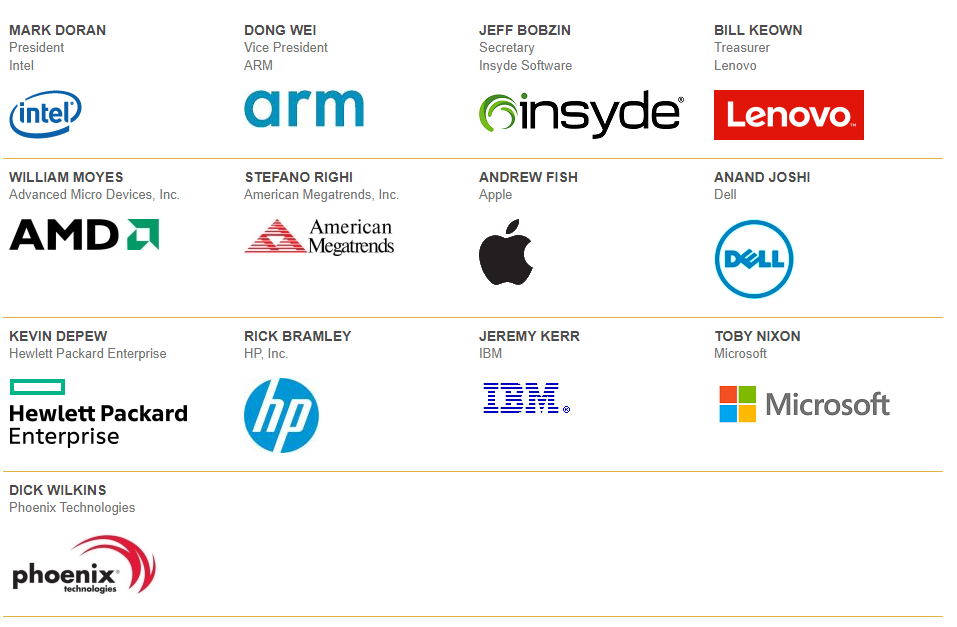
\includegraphics[width=\linewidth]{uefi_board_of_directors}
	\caption{Board of Directors of UEFI Forum}\label{fig:introduction-uefi-board-of-directors}
\end{figure}

The UEFI Forum board of directors consists of representatives from 11 industry leaders as described in Figure \ref{fig:introduction-uefi-board-of-directors}. These involved organizations work to ensure that the UEFI specifications meet industry needs.

UEFI uses a different interface for boot services and runtime services but UEFI does not specify how "Power On Self Test" (POST) and Setup are implemented - those are BIOS' primary functions.

\subsubsection{\gls{uefi} Driver Model Extension}
Access to boot devices is provided through a set of protocol interfaces. One purpose of the
UEFI Driver Model is to provide a replacement for \verb|PC-AT|-style option ROMs. It is important
to point out that drivers written to the UEFI Driver Model are designed to access boot devices in
the pre-boot environment. They are not designed to replace the high-performance, OS-specific
drivers.

The UEFI Driver Model is designed to support the execution of modular pieces of code,
also known as drivers, that run in the pre-boot environment. These drivers may manage or control
hardware buses and devices on the platform, or they may provide some software-derived, platform specific service. The UEFI Driver Model also contains information required by UEFI driver writers to design and implement any combination of bus drivers and device drivers that a platform
might need to boot a UEFI-compliant OS.

The UEFI Driver Model is designed to be generic and can be adapted to any type of bus or
device. The UEFI Specification describes how to write PCI bus drivers, PCI device drivers, USB
bus drivers, USB device drivers, and SCSI drivers. Additional details are provided that allow UEFI
drivers to be stored in PCI option ROMs, while maintaining compatibility with legacy option ROM
images.

One of the design goals in the UEFI Specification is keeping the driver images as small as
possible. However, if a driver is required to support multiple processor architectures, a driver
object file would also be required to be shipped for each supported processor architecture. To
address this space issue, this specification also defines the EFI Byte Code Virtual Machine. A
UEFI driver can be compiled into a single EFI Byte Code object file. UEFI Specificationcomplaint firmware must contain an EFI Byte Code interpreter. This allows a single EFI Byte
Code object file that supports multiple processor architectures to be shipped. Another space saving
technique is the use of compression. This specification defines compression and decompression
algorithms that may be used to reduce the size of UEFI Drivers, and thus reduce the overhead
when UEFI Drivers are stored in ROM devices.

The information contained in the UEFI Specification can be used by OSVs, IHVs, OEMs,
and firmware vendors to design and implement firmware conforming to this specification, drivers
that produce standard protocol interfaces, and operating system loaders that can be used to boot
UEFI compliant operating systems.

\subsubsection{\gls{uefi}'s Role in boot process}

During the boot process, UEFI speaks to the operating system loader and acts as the interface between the operating system and the BIOS.

The \verb|PC-AT| boot environment presents significant challenges to innovation within the
industry. Each new platform capability or hardware innovation requires firmware developers to
craft increasingly complex solutions, and often requires OS developers to make changes to their
boot code before customers can benefit from the innovation. This can be a time-consuming process
requiring a significant investment of resources. The primary goal of the UEFI specification is to
define an alternative boot environment that can alleviate some of these considerations. In this goal, the specification is like other existing boot specifications.

\subsection{Comparing of Legacy \gls{bios} and \gls{uefi}}

\begin{table}
	\centering
	\renewcommand{\arraystretch}{2}
	\caption{Legacy BIOS v/s UEFI}\label{table:legacy-bios-vs-uefi}
	\begin{tabular}{l | p{5cm} | p{5cm}}
		& Legacy BIOS & EFI
		\\ \hline \hline
		Language & Assembly & C ($ 99\% $)
		\\ \hline
		Resource & Interrupt Hardcode Memory Access hardcore I/O Access & Diver, Protocols
		\\ \hline
		Processor & x86 16-bit & CPU Protects Mode (Flat Mode)
		\\ \hline
		Expand & Hook Interrupt & Load Driver
		\\ \hline
		OS Bridge & ACPI & Run Time Driver Software
		\\ \hline
		$ 3^{rd} $ Party ISV \& IHV & Bas for Support & Easy for Support and for Multi Platforms
		\\ \hline
	\end{tabular}
\end{table}


\subsection{Advanced Configuration and Power Interface (\gls{acpi})}
The ACPI Component Architecture (ACPICA) defines and implements a group of software
components that together create an implementation of the ACPI specification. A major goal of the
architecture is to isolate all operating system dependencies to a relatively small translation or
conversion layer (the OS Services Layer) so that the bulk of the ACPICA code is independent of
any individual operating system. Therefore, hosting the ACPICA code on new operating systems
requires no source changes within the ACPICA code itself.

The components of the architecture include:
\begin{itemize}
	\item An OS-independent, kernel-resident ACPICA Subsystem component that provides the fundamental ACPI services such as the AML interpreter and namespace management.
	\item An OS-dependent OS Services Layer for each host operating system to provide OS support for the OS-independent ACPICA Subsystem.
	\item An ASL compiler-disassembler for translating ASL code to AML byte code and for disassembling existing binary ACPI tables back to ASL source code.
	\item Several ACPI utilities for executing the interpreter in ring 3 user space, extracting binary ACPI tables from the output of the ACPI Dump utility, and translating the ACPICA source	code to Linux/Unix format.
\end{itemize}

In Figure \ref{fig:introduction-acpi-component-architecture}, the ACPICA subsystem is shown in relation to the host operating system, device driver, OSPM software, and the ACPI hardware

\begin{figure}[h]
	\centering
	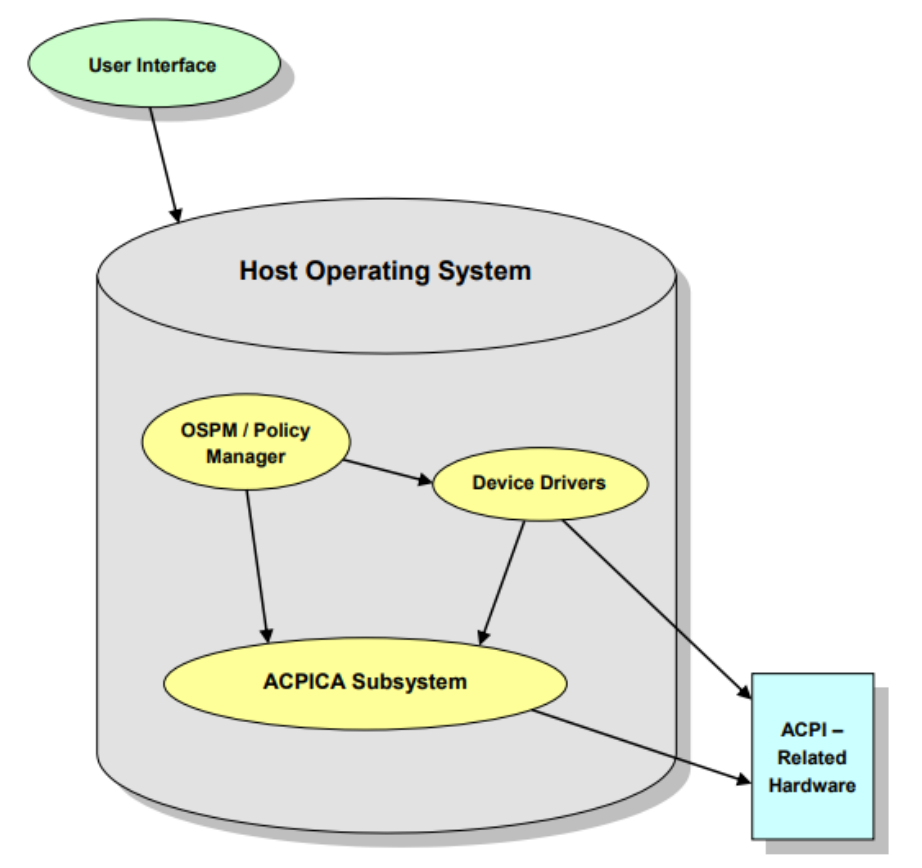
\includegraphics[width=0.7\linewidth]{introduction/acpi-component-architecture}
	\caption{The \gls{acpi} Component Architecture}\label{fig:introduction-acpi-component-architecture}
\end{figure}

\subsubsection{Overview of ACPICA Subsystem}
The ACPICA Subsystem implements the low level or fundamental aspects of the ACPI
specification. Included are an AML parser/interpreter, ACPI namespace management, ACPI table
and device support, and event handling. Since the ACPICA subsystem provides low-level system
services, it also requires low-level operating system services such as memory management,
synchronization, scheduling, and I/O.

To allow the ACPICA Subsystem to easily interface to any operating system that provides such
services, an Operating System Services Layer translates ACPICA-to-OS requests into the system
calls provided by the host operating system. The OS Services Layer is the only component of the
ACPICA that contains code that is specific to a host operating system.

Thus, the ACPICA Subsystem consists of two major software components:
\begin{itemize}
	\item The basic kernel-resident ACPICA Subsystem provides the fundamental ACPI services	that are independent of any particular operating system.
	\item The OS Services Layer (OSL) provides the conversion layer that interfaces the OS independent ACPICA Subsystem to a host operating system.
\end{itemize}

When combined into a single static or loadable software module such as a device driver or
kernel subsystem, these two major components form the ACPICA Subsystem. Throughout this
document, the term "ACPICA Subsystem" refers to the combination of the OS-independent
ACPICA Subsystem with an OS Services Layer components combined into a single module,
driver, or load unit.

\subsubsection{OS-independent ACPICA Subsystem}
The OS-independent ACPICA Subsystem supplies the major building blocks or subcomponents that are required for all ACPI implementations — including an AML interpreter, a namespace manager, ACPI event and resource management, and ACPI hardware support.

One of the goals of the ACPICA Subsystem is to provide an abstraction level high enough such
that the host operating system does not need to understand or know about the very low-level ACPI
details. For example, all AML code is hidden from the host. Also, the details of the ACPI hardware
are abstracted to higher-level software interfaces.

The ACPICA Subsystem implementation makes no assumptions about the host operating system or environment. The only way it can request operating system services is via interfaces provided by the OS Services Layer.

The primary user of the services provided by the ACPICA Subsystem are the host OS device drivers and power/thermal management software.

\subsubsection{Operating System Services Layer}
The OS Services Layer (or OSL) operates as a translation service for requests from the OS independent ACPICA subsystem back to the host OS. The OSL implements a generic set of OS service interfaces by using the primitives available from the host OS. Because of its nature.

The OS Services Layer must be implemented anew for each supported host operating
system. There is a single OS-independent ACPICA Subsystem, but there must be an OS Services
Layer for each operating system supported by the ACPI component architecture.

The primary function of the OSL in the ACPI Component Architecture is to be the small
glue layer that binds the much larger ACPICA Subsystem to the host operating system. Because
of the nature of ACPI itself — such as the requirement for an AML interpreter and management
of a large namespace data structure — most of the implementation of the ACPI specification is
independent of any operating system services. Therefore, the OS-independent ACPICA Subsystem
is the larger of the two components.

The overall ACPI Component Architecture in relation to the host operating system is Figure

\begin{figure}[h]
	\centering
	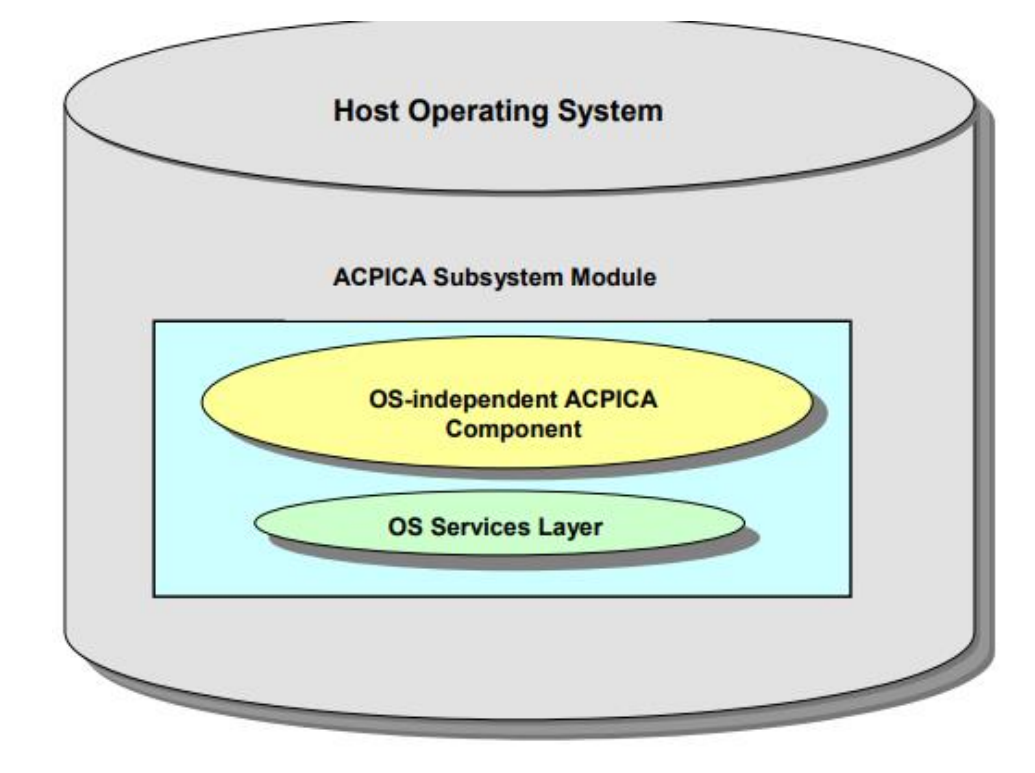
\includegraphics[width=0.7\linewidth]{introduction/acpica-subsystem-architecture}
	\caption{ACPICA Subsystem Architecture}\label{fig:introduction-acpica-subsystem-architecture}
\end{figure}

\subsubsection{ACPICA Subsystem Interaction}
The ACPICA Subsystem implements a set of external interfaces that can be directly called from
the host OS. These Acpi* interfaces provide the actual ACPI services for the host. When operating
system services are required during the servicing of an ACPI request, the Subsystem makes
requests to the host OS indirectly via the fixed AcpiOs* interfaces. The diagram below illustrates
the relationships and interaction between the various architectural elements by showing the flow
of control between them. Note that the OS-independent ACPICA Subsystem never calls the host directly instead it makes calls to the AcpiOs * interfaces in the OSL. This provides the ACPICA
code with OS-independence.

The Interaction between the Architectural Components Is shown in Figure \ref{fig:-introduction-acpi-interaction-between-the-architectural-components}

\begin{figure}[h]
	\centering
	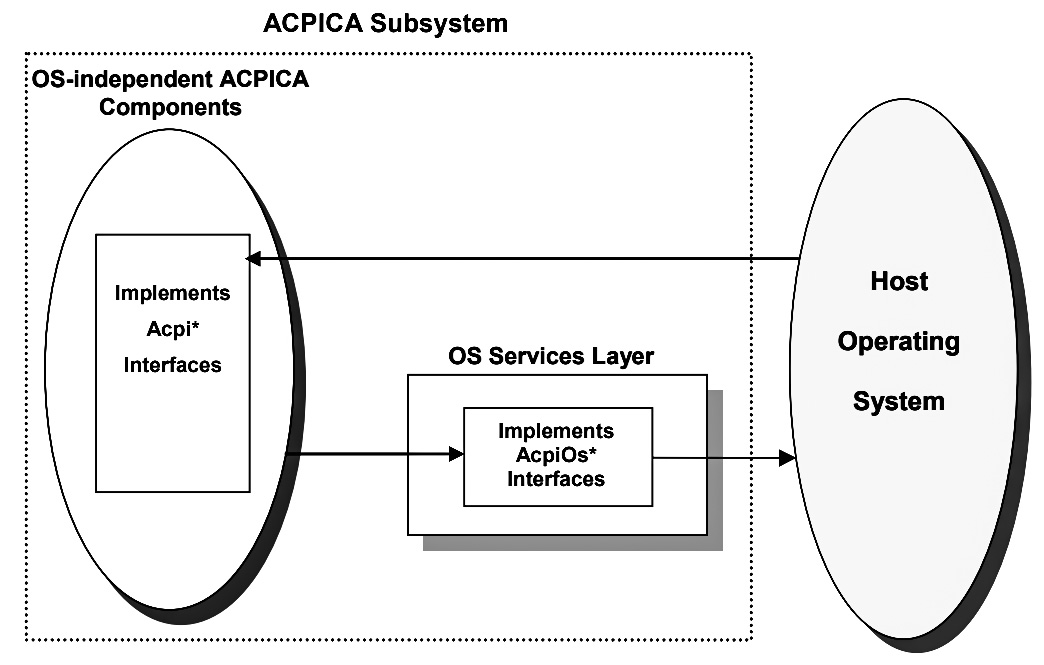
\includegraphics[width=0.7\linewidth]{introduction/acpi-interaction-between-the-architectural-components}
	\caption{Interaction between the Architectural Components}\label{fig:-introduction-acpi-interaction-between-the-architectural-components}
\end{figure}



\section{Design}

\subsection{\gls{uefi}/\gls{pi} Firmware Images}
\gls{uefi} and \gls{pi} specifications define the standardized format for EFI firmware storage devices (FLASH or other non-volatile storage) which are abstracted into "Firmware Volumes". Build systems must be capable of processing files to create the file formats described by the \gls{uefi} and PI specifications. The tools provided as part of the \gls{edk2} BaseTools package process files compiled by third party tools, as well as text and Unicode files in order to create UEFI or PI compliant binary image files. In some instances, where UEFI or PI specifications do not have an applicable input file format, such as the Visual Forms Representation (VFR) files used to create PI compliant IFR content, tools and documentation have been provided that allows the user to write text files that are processed into formats specified by UEFI or PI specifications.

\begin{figure}[h]
	\centering
	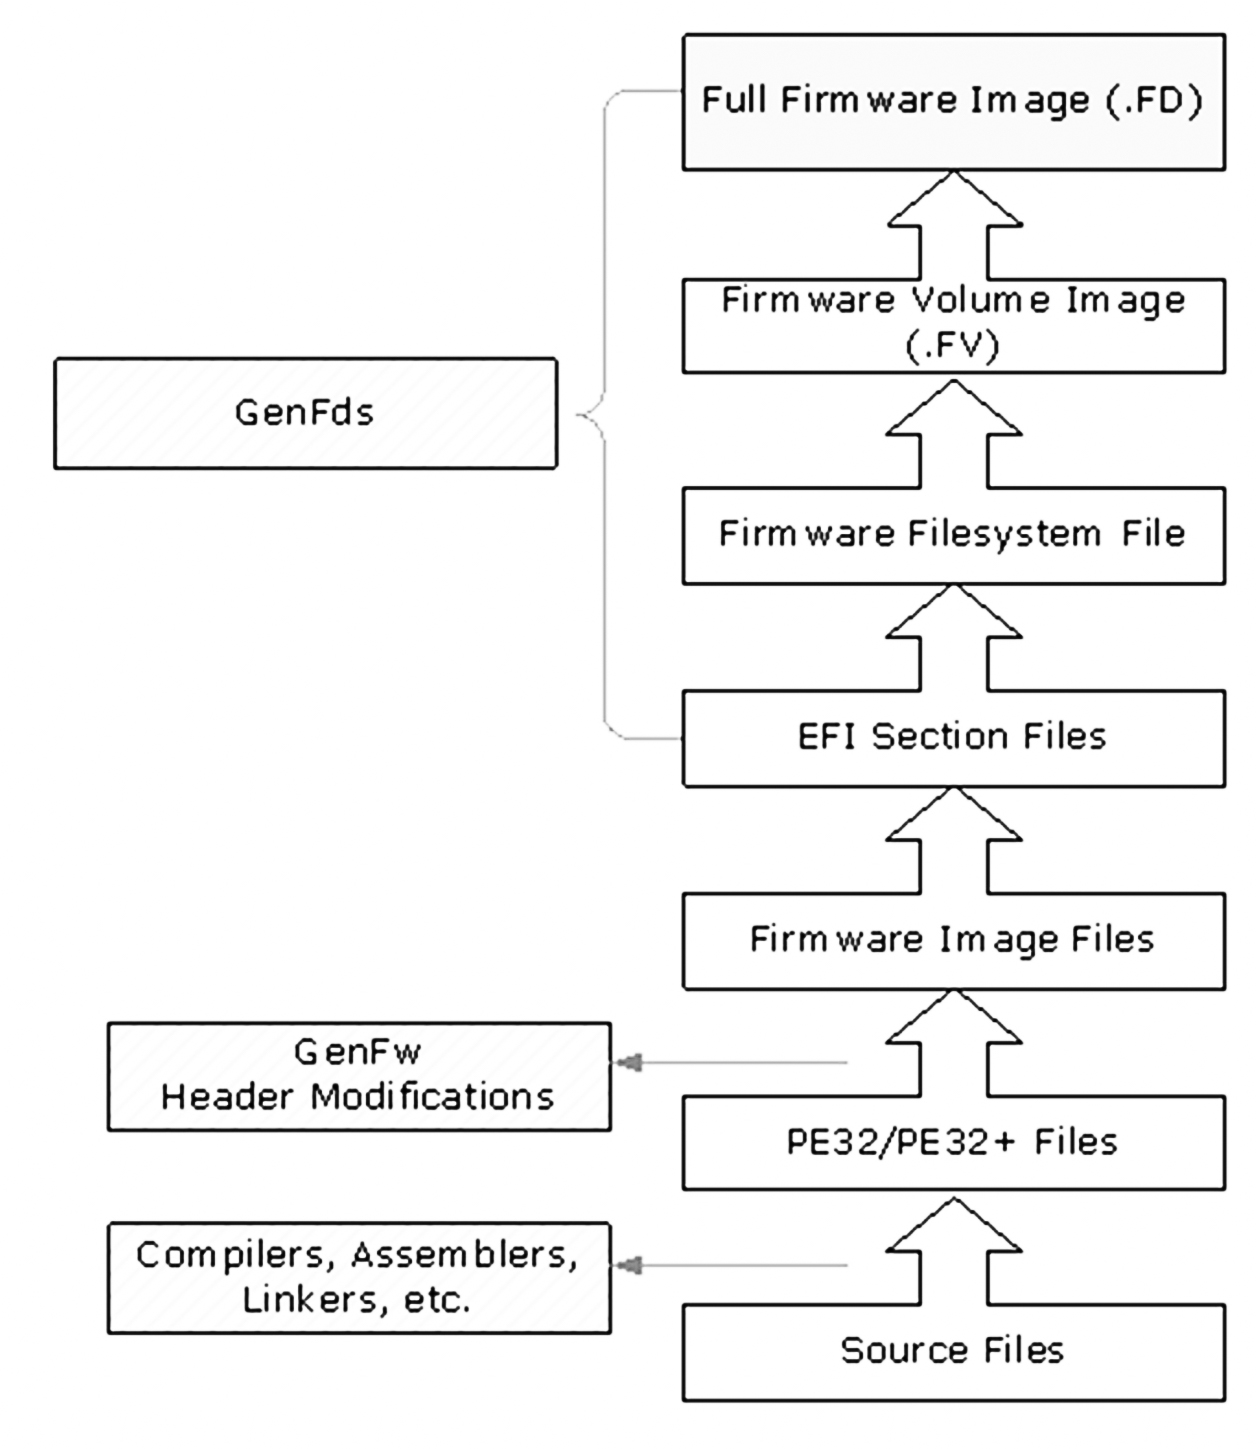
\includegraphics[width=0.7\linewidth]{design/uefi-pi-firmware-image-creation}
	\caption{UEFI/PI Firmware Image Creation}\label{fig:design-uefi-pi-firmware-image-creation}
\end{figure}

A Firmware Volume (FV) is a file level interface to firmware storage. Multiple FVs may be present in a single FLASH device, or a single FV may span multiple FLASH devices. An FV may be produced to support some other type of storage entirely, such as a disk partition or network device. For more information consult the Platform Initialization Specification, Volume 3.
In all cases, an FV is formatted with a binary file system. The file system used is typically the Firmware File System (FFS), but other file systems may be possible in some cases. Hence, all modules are stored as "files" in the FV. Some modules may be "execute in place" (linked at a fixed address and executed from the ROM), while others are relocated when they are loaded into memory and some modules may be able to run from ROM if memory is not present (at the time of the module load) or run from memory if it is available.
Files themselves have an internally defined binary format. This format allows for implementation of security, compression, signing, etc. Within this format, there are one or more "leaf" images. A leaf image could be, for example, a PE32 image for a DXE driver.

Therefore, there are several layers of organization to a full UEFI/PI firmware image. These layers are illustrated below in Figure \ref{fig:design-uefi-pi-firmware-image-creation}. Each transition between layers implies a processing step that transforms or combines previously processed files into the next higher level. Also shown in Figure \ref{fig:design-uefi-pi-firmware-image-creation} are the reference implementation tools that process the files to move them between the different layers.

\begin{figure}[h]
	\centering
	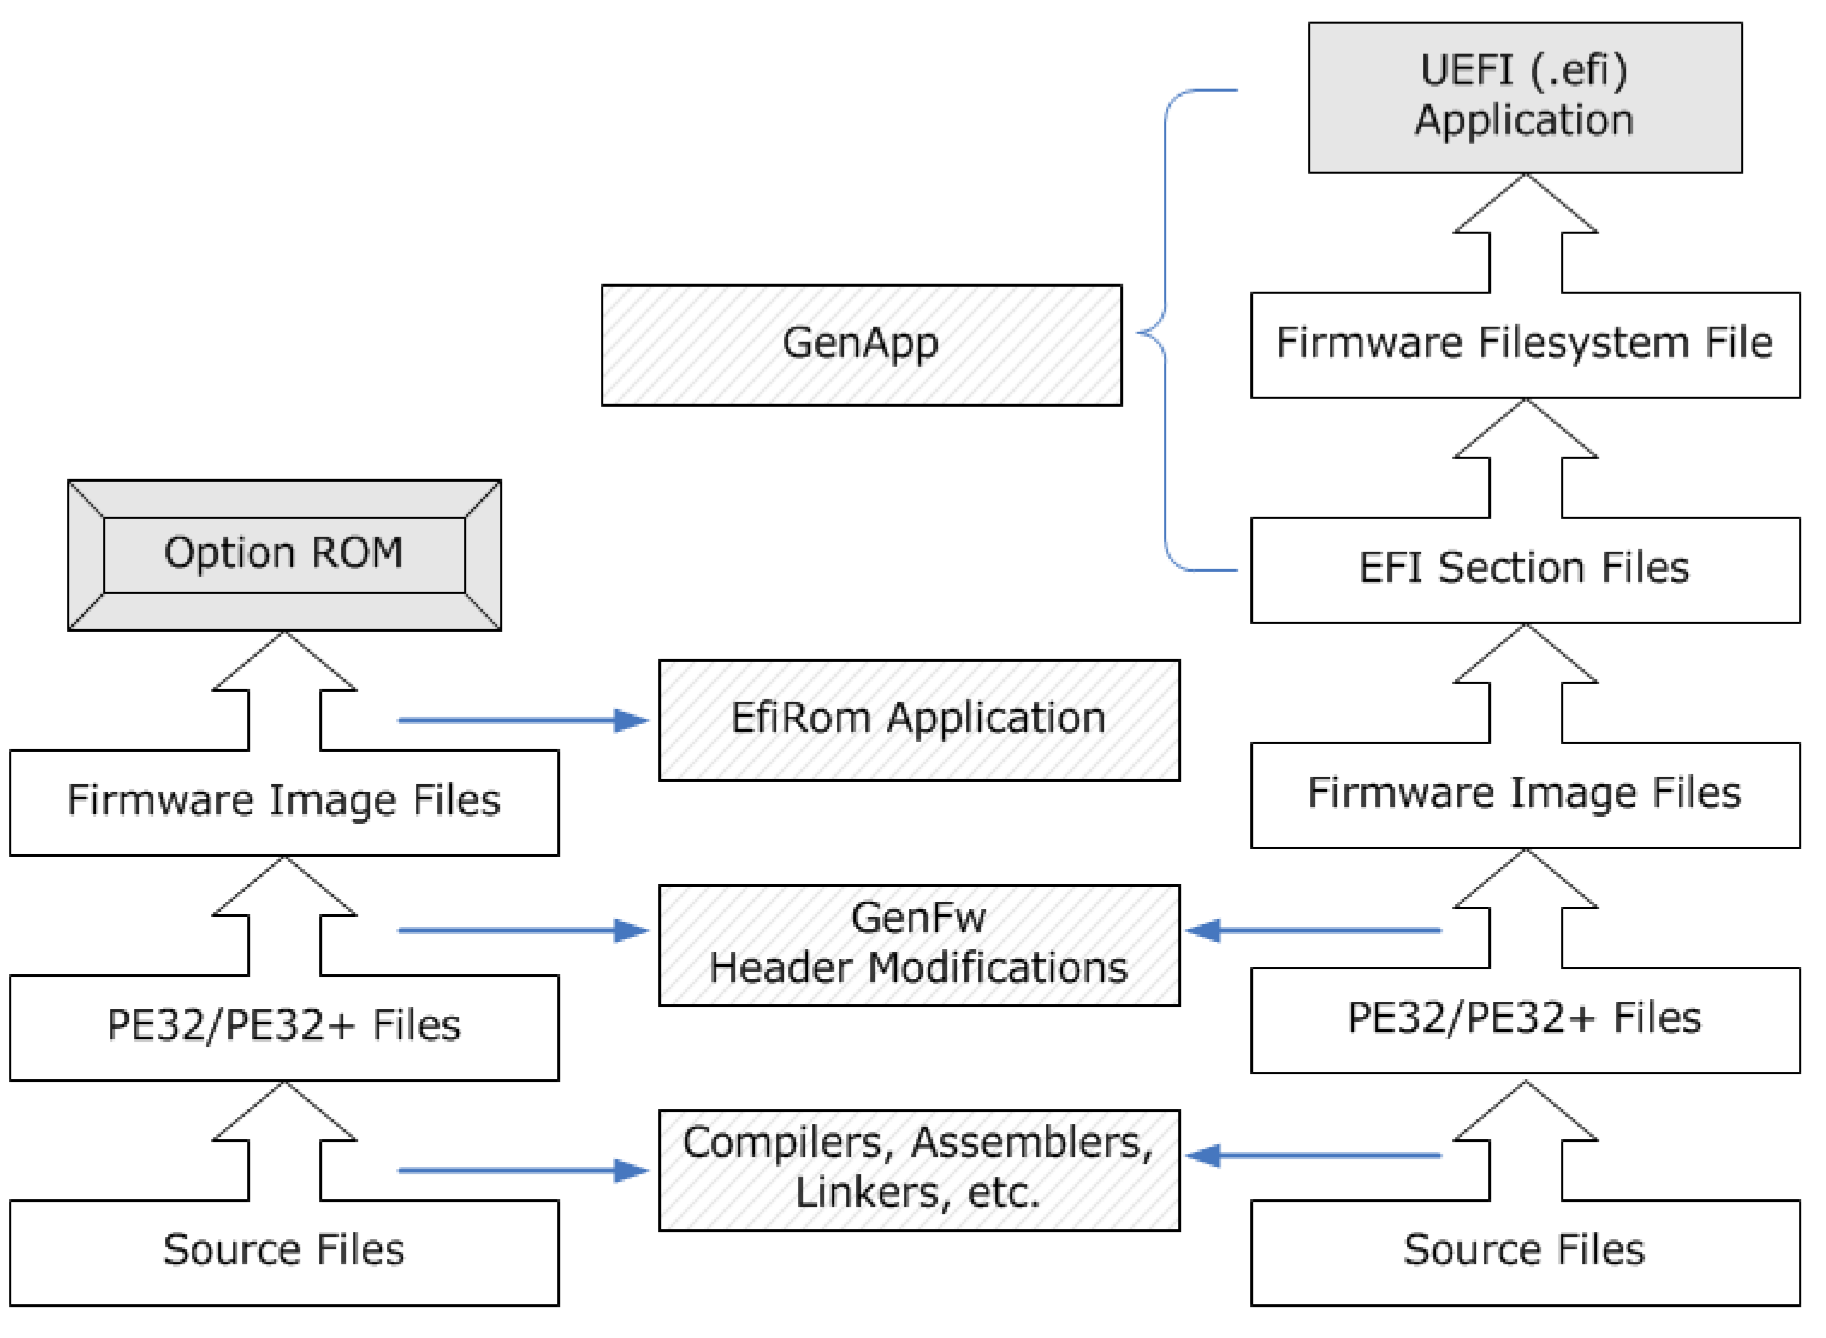
\includegraphics[width=0.7\linewidth]{design/efi-application-creation}
	\caption{UEFI/PI Firmware Image Creation}\label{fig:design-efi-application-creation}
\end{figure}


In addition to creating images that initialize a complete platform, the build process also supports creation of stand-alone UEFI applications (including OS Loaders) and Option ROM images containing driver code. Figure \ref{fig:design-efi-application-creation}, below, shows the reference implementation tools and creation processes for both of these image types

The final feature that is supported by the EDK II build process is the creation of Binary Modules that can be packaged and distributed for use by other organizations. Binary modules do not require distribution of the source code. This will permit vendors to distribute UEFI images without having to release proprietary source code.

This packaging process permits creation of an archive file containing one or more binary files that are either Firmware Image files or higher (EFI Section files, Firmware File system files, etc.). The build process will permit inserting these binary files into the appropriate level in the build stages.

\subsection{Platform Initialization \gls{pi} Boot Sequence}
PI compliant system firmware must support the six phases: security (\gls{sec}), pre-efi initialization (\gls{pei}), driver execution environment (\gls{dxe}), boot device selection (\gls{bds}), run time (RT) services and After Life (transition from the OS back to the firmware) of system. Refer to Figure \ref{fig:design-pi-boot-phases} below.

\begin{figure}[h]
	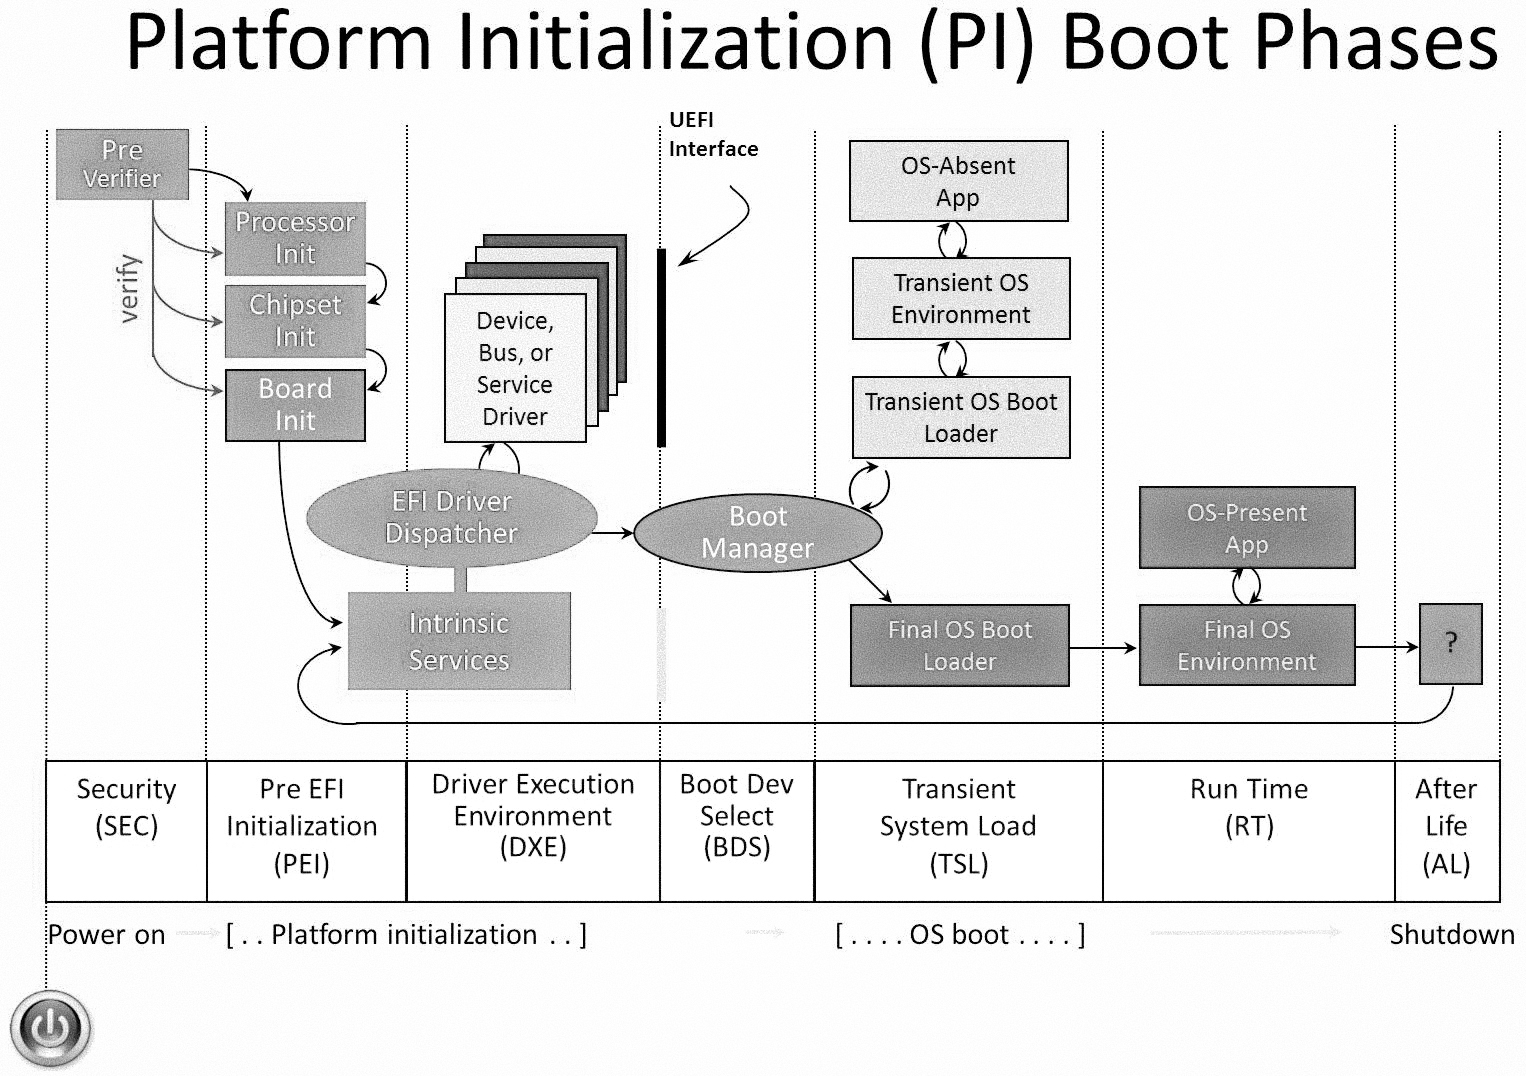
\includegraphics[width=\linewidth]{PI_Boot_Phases}
	\caption{\gls{pi} Boot Phases}\label{fig:design-pi-boot-phases}
\end{figure}

\subsection{Security (\gls{sec})}
The Security (SEC) phase is the first phase in the PI Architecture and is responsible for the following:
\begin{itemize}
	\item Handling all platform restart events
	\item Creating a temporary memory store
	\item Serving as the root of trust in the system
	\item Passing handoff information to the PEI Foundation
\end{itemize}
The security section may contain modules with code written in assembly. Therefore, some EDK II module development environment (MDE) modules may contain assembly code. Where this occurs, both Windows and GCC versions of assembly code are provided in different files

\subsection{Pre-EFI Initialization (\gls{pei})}
The Pre-EFI Initialization (PEI) phase described in the PI Architecture specifications is invoked quite betimes in the boot period. Specifically, after about preliminary processing in the Security (SEC) phase, any machine restart event will invoke the PEI phase.
The PEI phase is designed to be developed in many parts and consists of:
\begin{itemize}
	\item PEI Foundation (core code)
	\item Pre-EFI Initialization Modules (specialized plug-ins)
\end{itemize}
The PEI phase initially operates with the platform in a nascent state, leveraging only on-processor resources, such as the processor cache as a call stack, to dispatch Pre-EFI Initialization Modules (PEIMs).

The PEI phase cannot assume the availability of amounts of memory (RAM) as DXE and hence PEI phase limits its support to the following:
\begin{itemize}
	\item Locating and validating PEIMs
	\item Dispatching PEIMs
	\item Facilitating communication between PEIMs
	\item Providing handoff data to later phases
\end{itemize}

These PEIMs are responsible for the following:
\begin{itemize}
	\item Initializing some permanent memory complement
	\item Describing the memory in Hand-Off Blocks (HOBs)
	\item Describing the firmware volume locations in HOBs
	\item Passing control into the Driver Execution Environment (DXE) phase
\end{itemize}

Figure \ref{fig:design-pei-operation-diagram} shows a diagram describes the action carried out during the PEI phase

\begin{figure}[h]
	\centering
	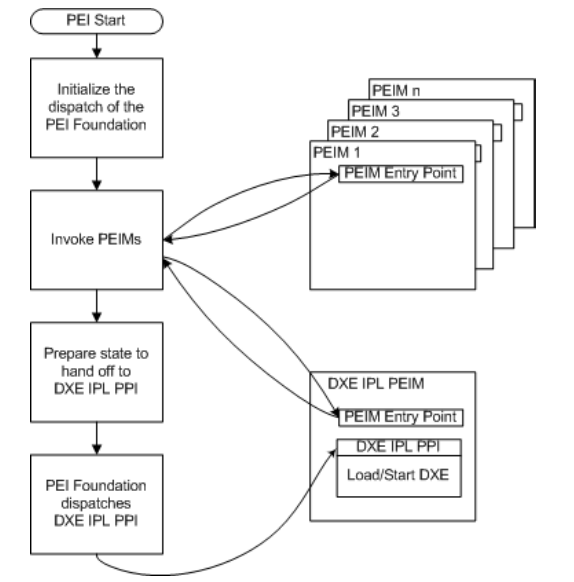
\includegraphics[width=0.7\linewidth]{design/pei-operation-diagram}
	\caption{Diagram of PI Operations}\label{fig:design-pei-operation-diagram}
\end{figure}

\subsubsection{PEI Services}
The PEI Foundation establishes a system table named the PEI Services Table that is visible to all Pre-EFI Initialization Modules (PEIMs) in the system. A PEI Service is defined as a function, command, or other capability manifested by the PEI Foundation when that service’s initialization requirements are met. Because the PEI phase has no permanent memory available until nearly the end of the phase, the range of services created during the PEI phase cannot be as rich as those created during later phases. Because the location of the PEI Foundation and its temporary RAM is not known at build time, a pointer to the PEI Services Table is passed into each PEIM’s entry point and also to part of each PEIM-to-PEIM Interface (PPI). 

The PEI Foundation provides the classes of services listed in Table \ref{table:design-pei-foundation-class-service}

\begin{table}[h]
	\centering
	\begin{tabular}{ l | p{8cm} }
		Service & Details
		\\ \hline \hline
		PPI Services & Manages PPIs to ease inter-module method calls between PEIMs. A database maintained in temporary RAM to track installed interfaces.
		\\ \hline
		Boot Mode Services & Manages the boot mode (S3, S5, diagnostics, normal boot, etc.)
		\\ \hline
		HOB Services & Creates data structures (Hand-off-blocks) that are used to convey information to the next phase 
		\\ \hline
		Firmware Volume Services & Finds PEIMs and along with that other firmware files in the firmware volumes
		\\ \hline
		PEI Memory Services & provides a collection of memory management services (to be used before and after permanent memory to discovered)
		\\ \hline
		Status Code Services & Provides general progress and error code reporting services (i.e. port 080h or a serial port for text output for debug)
		\\ \hline
		Reset Services & Provides a common means to aid initializing warm or cold restart of the system
		\\ \hline
	\end{tabular}
	\caption{Services provided by PEI Foundation Classes}\label{table:design-pei-foundation-class-service}
\end{table}


\subsubsection{PEI Foundation}
The PEI Foundation is the entity that carried outs following activity:
\begin{itemize}
	\item Dispatching of Pre-EFI initialization modules (PEIMs)
	\item Maintaining the boot mode
	\item Initialization of permanent memory
	\item Invoking the DXE loader 
\end{itemize}
The PEI Foundation written to be portable across all the various platforms architecture of a given instruction-set. i.e. A binary for IA-32 (32-bit Intel architecture) works across all Pentium processors and similarly Itanium processor family work across all Itanium processors.

Irrespective of the processor micro architecture, the set of services uncovered by the PEI Foundation should be the same. This consistent surface area around the PEI Foundation allows PEIMs to be written in the $C\ programming\ language$ and compiled across any micro architecture.

\subsection{PEI Dispatcher}
The PEI Dispatcher is basically a state machine which is implemented in the PEI Foundation. The PEI Dispatcher evaluates the dependency expressions in Pre-EFI initialization modules (PEIMs) that are lying in the \gls{fv}s being examined.

Dependency expressions are coherent combinations of PEIM-to-PEIM Interfaces (PPIs). These expressions distinguish the PPIs that must be available for use before a given PEIM can be invoked. The PEI Dispatcher references the PPI database in the PEI Foundation to conclude which PPIs have to be installed and evaluate the dependency expression for the PEIM. If PPI has already been installed then dependency expression will evaluate to $TRUE$, which notifies  PEI Dispatcher it can run PEIM. At this stage, the PEI Foundation handovers control to the PEIM with $TRUE$ dependency expression. 

The PEI Dispatcher will exit Once the PEI Dispatcher has examined and evaluated all of the PEIMs in all of the uncovered firmware volumes and no more PEIMs can be dispatched (i.e. the dependency expressions do not evaluate from $FALSE$ to $TRUE$). At this stage, the PEI Dispatcher cannot invoke any additional PEIMs. The PEI Foundation then takes back control from the PEI Dispatcher and invokes the $DXE IPL PPI$ to pass control to the DXE phase of execution.

\subsection{Drive Execution Environment (\gls{dxe})}
Prior to the DXE phase, the Pre-EFI Initialization (PEI) phase is responsible for initializing permanent memory in the platform so that the DXE phase can be loaded and executed. The state of the system at the end of the PEI phase is passed to the DXE phase through a list of position independent data structures called Hand-Off Blocks (HOBs). HOBs are described in detail in the Platform Initialization Specification.
There are several components in the DXE phase:
\begin{itemize}
	\item DXE Foundation
	\item DXE Dispatcher
	\item A set of DXE Drivers
\end{itemize}

\subsection{Boot Device Selection (\gls{bds})}
The Boot Device Selection (BDS) phase is implemented as part of the BDS Architectural Protocol. The DXE Foundation will hand control to the BDS Architectural Protocol after all of the DXE drivers whose dependencies have been satisfied have been loaded and executed by the DXE Dispatcher. The BDS phase is responsible for the following:
\begin{itemize}
	\item Initializing console devices
	\item Loading device drivers
	\item Attempting to load and execute boot selections
\end{itemize}

\subsection{Transient System Load (TSL) and Runtime (RT)}
The Transient System Load (TSL) is primarily the OS vendor provided boot loader. Both the TSL and the Runtime Services (RT) phases may allow access to persistent content, via UEFI drivers and UEFI applications. Drivers in this category include PCI Option ROMs.

\subsection{After Life (AL)}
The After Life (AL) phase consists of persistent UEFI drivers used for storing the state of the system during the OS orderly shutdown, sleep, hibernate or restart processes.



\subsection{Generic Build Process}
All code starts out as either C sources and header files, assembly sources and header files, UCS-2 HII strings in Unicode files, Virtual Forms Representation files or binary data (native instructions, such as microcode) files. Per the UEFI and PI specifications, the C and Assembly files must be compiled and linked into PE32/PE32+ images.
While some code is designed to execute only from ROM, most UEFI/PI modules are written to be relocate-able. These are written and built different. For example, Execute In Place (XIP) module code is written and compiled to run from ROM, while the majority of the code is written and compiled to execute from memory, which requires that the code be relocate able.
Some modules may also permit dual mode, where it will execute from memory only if memory is available, otherwise it will execute from ROM. Additionally, modules may permit dual access, such as a driver that contains both PEI and DXE implementation code. Code is assembled or compiled, then linked into PE32/PE32+ images, the relocation section may or may not be stripped and an appropriate header will replace the PE32/PE32+ header. Additional processing may remove more non-essential information, generating a Terse (TE) image.
The binary executables are converted into EFI firmware file sections. Each module is converted into an EFI Section consisting of an Section header followed by the section data (driver binary).

\subsubsection{EFI Section Files}
he general section format for sections less than 16MB in size is shown in Figure \ref{fig:design-general-efi-section-format}. Figure \ref{fig:design-general-efi-section-format-large} shows the section format for sections 16MB or larger in size using the extended length field.

\begin{figure}[h]
	\centering
	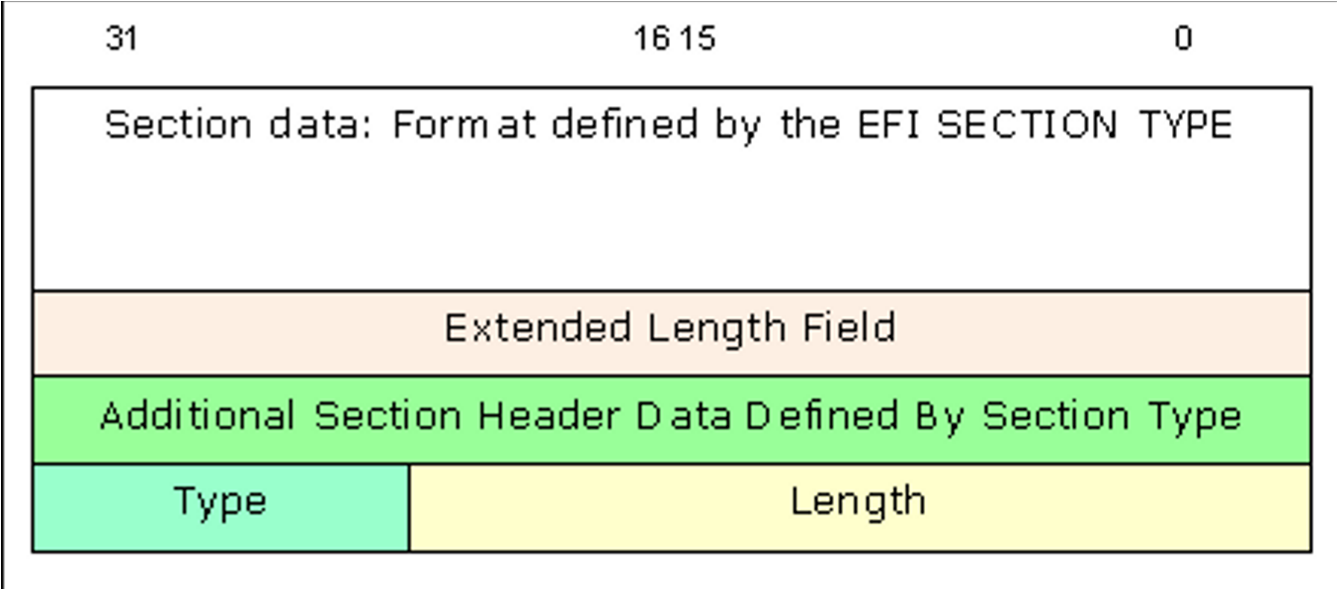
\includegraphics[width=0.7\linewidth]{design/general-efi-section-format-large}
	\caption{General EFI Section Format for large size Sections(greater then 16 MB)}\label{fig:design-general-efi-section-format-large}
\end{figure}


\begin{figure}[h]
	\centering
	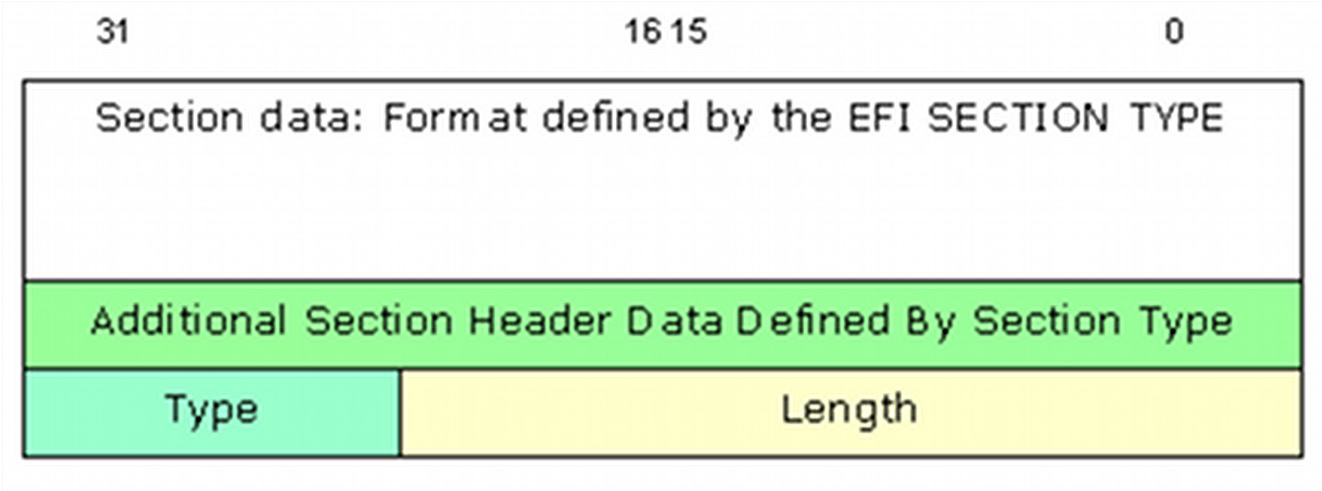
\includegraphics[width=0.7\linewidth]{design/general-efi-section-format}
	\caption{General EFI Section Format (less then 16 MB)}\label{fig:design-general-efi-section-format}
\end{figure}



\subsection{Cross Compatibility of CPUs}
Whenever customer try to change the default Intel motherboard CPU with different Intel silicon chip which won’t works. The specific CPU Chip initialization varies for each generation. So, the board designs should be designed is such a way that specific generation CPU should support., if we change the CPU with a different Intel Board it will not even boot, because the BIOS doesn't support for other Silicon Initialization for other CPUs.

So, we are integrating the runtime detection of the silicon during the Pre-Extensible Firmware Initialization (\gls{pei}) phase. So, within single Integrated Firmware Image (\gls{ifwi}) should support the Multi Generation CPUs which is never tried before.

Each silicon has a fixed register from which the CPU generation can be identified., so the BIOS should read that register and program in such a way the is CPU1 is in Platform it should support the CPU1 Features like PCIe, Graphics \& DMI., if the CPU1 is replaced with CPU2 then it should support the CPU2 speed. That should be taken care by the BIOS.

\begin{figure}[h]
	\centering
	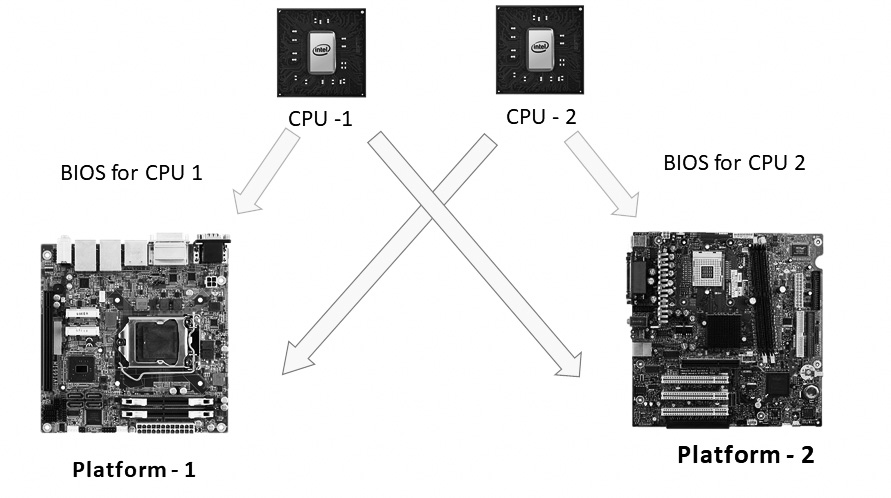
\includegraphics[width=0.7\linewidth]{design/cross-compatibility-design}
	\caption{Cross Compatibility Design}\label{fig:design-cross-compatibility-design}
\end{figure}

Figure \ref{fig:design-cross-compatibility-design} shows the general view of the Cross Compatibility of CPUs.

BIOS is the part of Integrated Firmware Image which resides at the End of the Binary table. The CPU swap can only occur in Specially designed Intel Designed Board only. Mainly because for each and every feature it required some hardware(H/W) requirements. If that H/W requirement not present. Then It will boot but doesn't support the Maximum speed.


\begin{figure}[h]
	\centering
	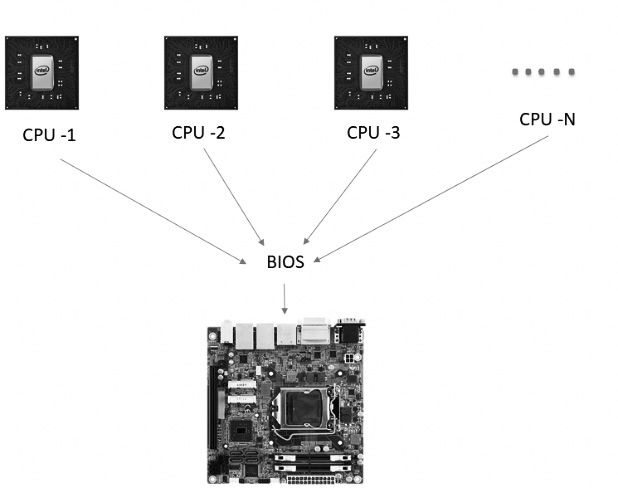
\includegraphics[width=0.7\linewidth]{design/bios-support-for-cross-compatibility}
	\caption{BIOS Support for Cross Compatibility}\label{fig:design-bios-support-for-cross-compatibility}
\end{figure}

Figure \ref{fig:design-bios-support-for-cross-compatibility} shows the BIOS role for identifying the CPUs during PEI phase.

As the number of Feature increases in the Silicon BIOS size also increases, usually the BIOS size varies from Platform to Platform and CPU to CPU., as we are integrating the Compatibility the BIOS size obviously increases. 

The structure of \gls{ifwi} is Shown in Figure \ref{fig:design-integrated-firmware-image}

\begin{figure}[h]
	\centering
	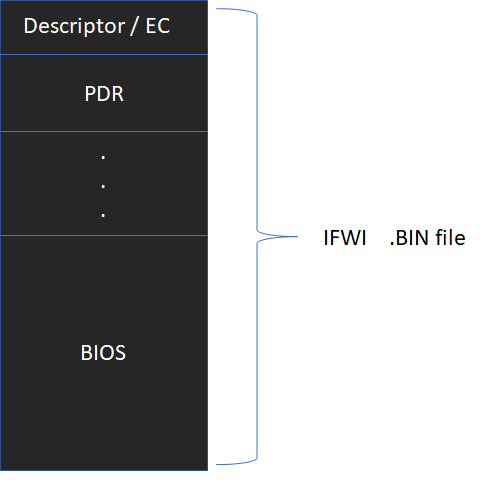
\includegraphics[width=0.7\linewidth]{design/integrated-firmware-image}
	\caption{Integrated Firmware Image}\label{fig:design-integrated-firmware-image}
\end{figure}



\section{Architecture of BIOS Firmware}\label{section-architecture}
\subsection{Overview}
The basic Platform Initialization firmware storage concepts include:
\begin{itemize}
	\item Firmware Volumes (\gls{fv})
	\item Firmware File Systems (\gls{ffs})
	\item Firmware Files
	\item Standard Binary Layout
	\item Pre-EFI Initialization (\gls{pei}) PEIM-to-PEIM Interfaces (PPIs)
	\item Driver Execution Environment (\gls{dxe}) Protocols
\end{itemize}

\subsection{Design of Firmware Storage}
Design of firmware storage describes how files should be stored and accessed in non-volatile storage. Implementation of any firmware must support and follow the standard \gls{pi} Firmware Volume structure and the structure of Firmware File System Format.

\paragraph{Firmware Device} is a persistent physical repository containing data and/or firmware code. Typically it is a flash component but may also be some other type of persistent storage. A single physical firmware device may be partitioned into multiple smaller pieces to form multiple logical firmware devices. Likewise, multiple firmware devices may be aggregated into one larger logical firmware device.

\paragraph{Flash} devices are most usual non-volatile repository for firmware volumes. Often, flash devices are partitioned into sectors or blocks of possibly differing sizes, each with various run-time characteristics.

In the design of Firmware File System (\gls{ffs}), several observed unique qualities of flash devices are listed below:
\begin{itemize}
	\item Can be erased on a sector-by-sector basis. After ensuring, all bits of sector return their \verb|erase value|\footnote{either all $0$ or all $1$}.
	\item Can be written on a bit-by-bit basis. i.e. if erase value is $ 0 $ then bit value $ 0 $ can be changed to $ 1 $.
	\item Only by performing erase operation on an entire flash sector, \verb|non-erase value| can change to \verb|erase value|.
	\item Capable of enable/disable reads and writes to individual flash sectors or the entire flash.
	\item Writes and erases are longer operations than reads.
	\item Many times place restrictions on the trading operations that can be performed while a write or erase is occurring.
\end{itemize}

\subsection{Firmware Volumes (\gls{fv})}
A Firmware Volume (\gls{fv}) is a logical firmware device. Firmware Volume is the basic storage repository for data and/or code. Each and every firmware volume is organized into a file system. As such, the file is the base unit of storage for firmware.
Table \ref{table:firmware-volume-attributes} describes attributes in each firmware volume.

\begin{table}[!htbp]
	\centering
	\renewcommand{\arraystretch}{2}
	\caption{Firmware Volume Attributes}\label{table:firmware-volume-attributes}
	\begin{tabular}{p{4cm} | p{11cm}}
		\textbf{Attribute} & \textbf{Description}
		\\ \hline \hline
		Name & each volume has a unique identifier name having UEFI Globally Unique Identifier (GUID). 
		\\ \hline
		Size & describes total size of all volume data (including any header, files and free space)
		\\ \hline
		Format & describes Firmware File System (FFS) used in the body of the volume.
		\\ \hline
		Memory Mapped? & some volumes may be memory-mapped, indicates that the entire contents of the volume appear at once in the memory address space of the processor. 
		\\ \hline
		Sticky Write? & Some volumes may require special erase cycles in order to change bits from a
		non-erase value to an erase value
		\\ \hline
		Erase Polarity & If a volume supports \textit{Sticky Write}, then all bits within the volume will return
		to this value (0 or 1) after an erase cycle
		\\ \hline
		Alignment & The first byte of a volume is required to be aligned on some power-of-two
		boundary. At a minimum, this must be greater than or equal to the highest file alignment value.
		If \verb|EFI_FVB2_WEAK_ALIGNMENT| is set in the volume header then the first byte of the volume
		can be aligned on any power-of-two boundary. A weakly aligned volume can not be moved from
		its initial linked location and maintain its alignment.
		\\ \hline
		Read Enable/Disable Capable/Status & Volumes may have the ability to change from readable
		to hidden
		\\ \hline
		Write Enable/Disable Capable/Status & Volumes may have the ability to change from writable
		to write protected
		\\ \hline
		Lock Capable/Status & Volumes may be able to have their capabilities locked
		\\ \hline
		Read-Lock Capable/Status & Volumes may have the ability to lock their read status
		\\ \hline
		Write-Lock Capable/Status & Volumes may have the ability to lock their write status
		\\ \hline
	\end{tabular}
\end{table}

Firmware volumes may also contain additional information describing the mapping between OEM
file types and a \verb|GUID|.

\subsection{Firmware File System (\gls{ffs})}
A Firmware File System (\gls{ffs}) describes the structure of files and (optional) free space within the firmware volume. Each firmware file systems has a unique GUID, which is used by the firmware to associate a driver with a newly exposed firmware volume.


\begin{table}[h]
	\centering
	\renewcommand{\arraystretch}{2}
	\caption{Firmware Files Attributes}\label{table:firmware-files-attributes}
	\begin{tabular}{p{4cm} | p{11cm}}
		\textbf{Attribute} & \textbf{Description}
		\\ \hline \hline
		Name & each volume has a unique identifier name having UEFI Globally Unique Identifier (GUID). File names must be unique within a firmware volume. Some file names have special significance.
		\\ \hline
		Type & Each file has a type. There are four ranges of file types: Normal (0x00-0xBF), OEM	(0xC0-0xDF), Debug (0xE0-0xEF) and Firmware Volume Specific (0xF0-0xFF). More file types information are described in Table \ref{table:firmware-file-types}.
		\\ \hline
		Alignment & Each file’s data can be aligned on some power-of-two boundary. The specific boundaries that are supported depend on the alignment and format of the firmware volume. If \verb|EFI_FVB2_WEAK_ALIGNMENT| is set in the volume header then file alignment does not
		\\ \hline
		Size & Describes size of each file, each file's data is zero or more bytes
		\\ \hline
	\end{tabular}
\end{table}

Firmware files are code and/or data stored in firmware volumes. Attributes of files are described in Table \ref{table:firmware-files-attributes}.

Specific firmware volume formats may support additional attributes, such as integrity verification and staged file creation. The file data of certain file types is sub-divided in a standardized fashion into Firmware File Sections.

Non-standard file types are supported through the use of the OEM file types (described in detail in Table \ref{table:firmware-file-types}).

In the PEI phase, file-related services are provided through the PEI Services Table, using \verb|FfsFindNextFile|, \verb|FfsFindFileByName| and \verb|FfsGetFileInfo|. In the DXE phase, file related services are provided through the \\ \verb|EFI_FIRMWARE_VOLUME2_PROTOCOL| services attached to a volume's handle (\verb|ReadFile|, \verb|ReadSection|, \verb|WriteFile| and \verb|GetNextFile|).

\subsubsection{Firmware File Types}
Consider an application file named FOO.EXE. The format of the contents of \verb|FOO.EXE| is implied by the ".EXE" in the file name. Depending on the operating environment, this extension typically indicates that the contents of FOO.EXE are a PE/COFF image and follow the PE/COFF image format.

Similarly, the PI Firmware File System defines the contents of a file that is returned by the firmware volume interface.

The PI Firmware File System defines an enumeration of file types. For example, the type
\verb|EFI_FV_FILETYPE_DRIVER| indicates that the file is a DXE driver and is interesting to the DXE
Dispatcher. In the same way, files with the type \verb|EFI_FV_FILETYPE_PEIM| are interesting to the
PEI Dispatcher.

\begin{table}[!htbp]
	\centering
	\renewcommand{\arraystretch}{1.2}
	\caption{Firmware File Types}\label{table:firmware-file-types}
	\begin{tabular}{l | p{1cm} | p{6cm}}
		Name & Value & Description
		\\ \hline \hline
		\verb|FV_FILETYPE_RAW| & $ 0x1 $ & Binary Data
		\\ \hline
		\verb|FV_FILETYPE_FREEFORM| & $ 0x2 $ & Sectioned Data
		\\ \hline
		\verb|FV_FILETYPE_SECURITY_CORE| & $ 0x3 $ & Platform core code used during the SEC phase
		\\ \hline
		\verb|FV_FILETYPE_PEI_CORE| & $ 0x4 $ & PEI Foundation
		\\ \hline
		\verb|FV_FILETYPE_DXE_CORE| & $ 0x5 $ & DXE Foundation
		\\ \hline
		\verb|FV_FILETYPE_PEIM| & $ 0x6 $ & PEI Module (PEIM)
		\\ \hline
		\verb|FV_FILETYPE_DRIVER| & $ 0x7 $ & DXE Driver
		\\ \hline
		\verb|FV_FILETYPE_COMBINED_PEIM_DRIVER| & $ 0x8 $ & Combined PEIM/DXE Driver
		\\ \hline
		\verb|FV_FILETYPE_APPLICATION| & $ 0x9 $ & Application
		\\ \hline
		\verb|FV_FILETYPE_SMM| & $ 0xa $ & Contains a PE32+ image that will be loaded into MMRAM in MM Traditional Mode
		\\ \hline
		\verb|FV_FILETYPE_FIRMWARE_VOLUME_IMAGE| & $ 0xb $ & Firmware Volume Image
		\\ \hline
		\verb|FV_FILETYPE_COMBINED_SMM_DXE| & $ 0xc $ & Contains PE32+ image that will be dispatched by the DXE Dispatcher and will also be loaded into MMRAM in MM Tradition Mode
		\\ \hline
		\verb|FV_FILETYPE_SMM_CORE| & $ 0xd $ & MM Foundation that support MM Traditional Mode
		\\ \hline
		\verb|EFI_FV_FILETYPE_MM_STANDALONE| & $ 0xe $ & Contains PE32+ image that will be loaded into MMRAM in MM Standalone Mode
		\\ \hline
		\verb|EFI_FV_FILETYPE_MM_CORE_STANDALONE| & $ 0xf $ & Contains PE32+ image that support MM Tradition Mode and MM Standalone Mode
		\\ \hline
		\verb|FV_FILETYPE_OEM_MIN| & $ 0xc0 $ & OEM File Type
		\\ \hline
		\verb|FV_FILETYPE_OEM_MAX| & $ 0xdf $ & OEM File Type
		\\ \hline
		\verb|FV_FILETYPE_DEBUG_MIN| & $ 0xe0 $ & Debug/Test File Type
		\\ \hline
		\verb|FV_FILETYPE_DEBUG_MAX| & $ 0xef $ & Debug/Test File Type
		\\ \hline
		\verb|FV_FILETYPE_FFS_MIN| & $ 0xf0 $ & Firmware File System Specific File Type
		\\ \hline
		\verb|FV_FILETYPE_FFS_MAX| & $ 0xff $ & Firmware File System Specific File Type
		\\ \hline
		\verb|FV_FILETYPE_FFS_PAD| & $ 0xf0 $ & Pad file for FFS
		\\ \hline
	\end{tabular}
\end{table}

\subsection{Firmware File Sections}
Firmware file sections are separate discrete “parts” within certain file types. Each section has the
following attributes:
\begin{table}[!htbp]
	\begin{tabular}{l | p{9cm}}
		Attribute & Description
		\\ \hline \hline
		Type & Each section has type 
		\\ \hline
		Size & describes size of the section
		\\ \hline
	\end{tabular}
\end{table}

While there are many types of sections, they fall into the following two broad categories:
\begin{itemize}
	\item \textbf{Encapsulation sections} - containers that hold other sections.
	The sections contained within an encapsulation section are known as child sections, and the encapsulation section is known as the parent section are known as the parent section. An encapsulation section's	children may be leaves and/or more encapsulation sections and are called peers relative to each other. An encapsulation section does not contain data directly; instead it is just a vessel that ultimately terminates in leaf sections. Files that are built with sections can be thought of as a tree, with encapsulation sections as nodes and	leaf sections as the leaves. The file image itself can be thought of as the root and may contain an arbitrary number of sections. Sections that exist in the root have no parent section but are still considered peers.
	\item \textbf{Leaf Sections} - Unlike encapsulation sections, leaf sections directly contain data and do not contain other sections. The format of the data contained within a leaf section is defined by the type of the section.
\end{itemize}

\begin{figure}[!htbp]
	\centering
	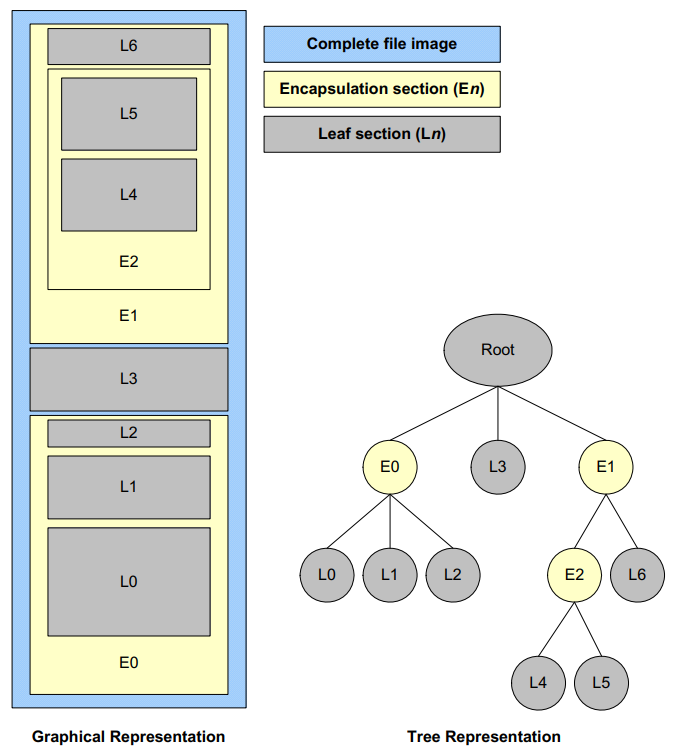
\includegraphics[width=0.9\linewidth]{architecture/firmware-file-system-representation}
	\caption{Example File System Image}\label{fig:architecture-firmware-file-system-representation}
\end{figure}

In the example shown in Figure \ref{fig:architecture-firmware-file-system-representation}, the file image root contains two encapsulation sections (E0 and E1) and one leaf section (L3). The first encapsulation section (E0) contains children, all of which are leaves (L0, L1, and L2). The second encapsulation section (E1) contains two children, one that is an encapsulation (E2) and the other that is a leaf (L6). The last encapsulation section (E2) has two children that are both leaves (L4 and L5).

In the PEI phase, section-related services are provided through the PEI Service Table, using \verb|FfsFindSectionData|. In the DXE phase, section-related services are provided through the \verb|EFI_FIRMWARE_VOLUME2_PROTOCOL| services attached to a volume's handle (\verb|ReadSection|).

\subsection{Firmware File Section Types}
Table \ref{table:architectural-section-types} list outs the defined architectural section types.

\begin{table}[!htbp]
	\centering
	\renewcommand{\arraystretch}{1.2}
	\caption{Architectural Section Types}\label{table:architectural-section-types}
	\begin{tabular}{p{7cm} | l | p{5cm}}
		Name & Value & Description
		\\ \hline \hline
		\verb|EFI_SECTION_COMPRESSION| & $ 0x1 $ & Encapsulation section where other sections are compressed
		\\ \hline
		\verb|EFI_SECTION_GUID_DEFINED| & $ 0x2 $ & Encapsulation section used during the build process but not required for execution
		\\ \hline
		\verb|EFI_SECTION_DISPOSABLE| & $ 0x3 $ & Encapsulation section used during the build process but not required for execution
		\\ \hline
		\verb|EFI_SECTION_PE32| & $ 0x10 $ & PE32+ Executable image
		\\ \hline
		\verb|EFI_SECTION_PIC| & $ 0x11 $ & Position-Independent Code
		\\ \hline
		\verb|EFI_SECTION_TE| & $ 0x12 $ & Terse Executable Image
		\\ \hline
		\verb|EFI_SECTION_DXE_DEPEX| & $ 0x13 $ & DXE Dependency Expression
		\\ \hline
		\verb|EFI_SECTION_VERSION| & $ 0x14 $ & Version, Text and numeric
		\\ \hline
		\verb|EFI_SECTION_USER_INTERFACE| & $ 0x15 $ & User-Friendly name of the driver
		\\ \hline
		\verb|EFI_SECTION_COMPATIBILITY16| & $ 0x16 $ & DOS-style 16-bit EXE
		\\ \hline
		\verb|EFI_SECTION_FIRMWARE_VOLUME_IMAGE| & $ 0x17 $ & PI Firmware Volume Image
		\\ \hline
		\verb|EFI_SECTION_FREEFORM_SUBTYPE_GUID| & $ 0x18 $ & Raw data with GUID in header to define format
		\\ \hline
		\verb|EFI_SECTION_RAW| & $ 0x19 $ & Raw data
		\\ \hline
		\verb|EFI_SECTION_PEI_DEPEX| & $ 0x1b $ & PEI Dependency Expression
		\\ \hline
		\verb|EFI_SECTION_SMM_DEPEX| & $ 0x1c $ & Leaf section type for determining the dispatch order for an MM Traditional driver in MM Traditional Mode or MM Standalone driver in MM Standalone Mode.
		\\ \hline
	\end{tabular}
\end{table}

\subsection{PI Architecture Firmware File System Format}
This section describes the standard binary encoding for PI Firmware Files, PI Firmware Volumes, and the PI Firmware File System. Implementations that allow the non-vendor firmware files or firmware volumes to be introduced into the system must support the standard formats. This section also describes how features of the standard format map into the standard PEI and DXE interfaces.

The standard firmware file and volume format also introduces additional attributes and capabilities that are used to guarantee the integrity of the firmware volume. The standard format is broken into three levels: the firmware volume format, the firmware file system format, and the firmware file format.

\begin{figure}[!htbp]
	\centering
	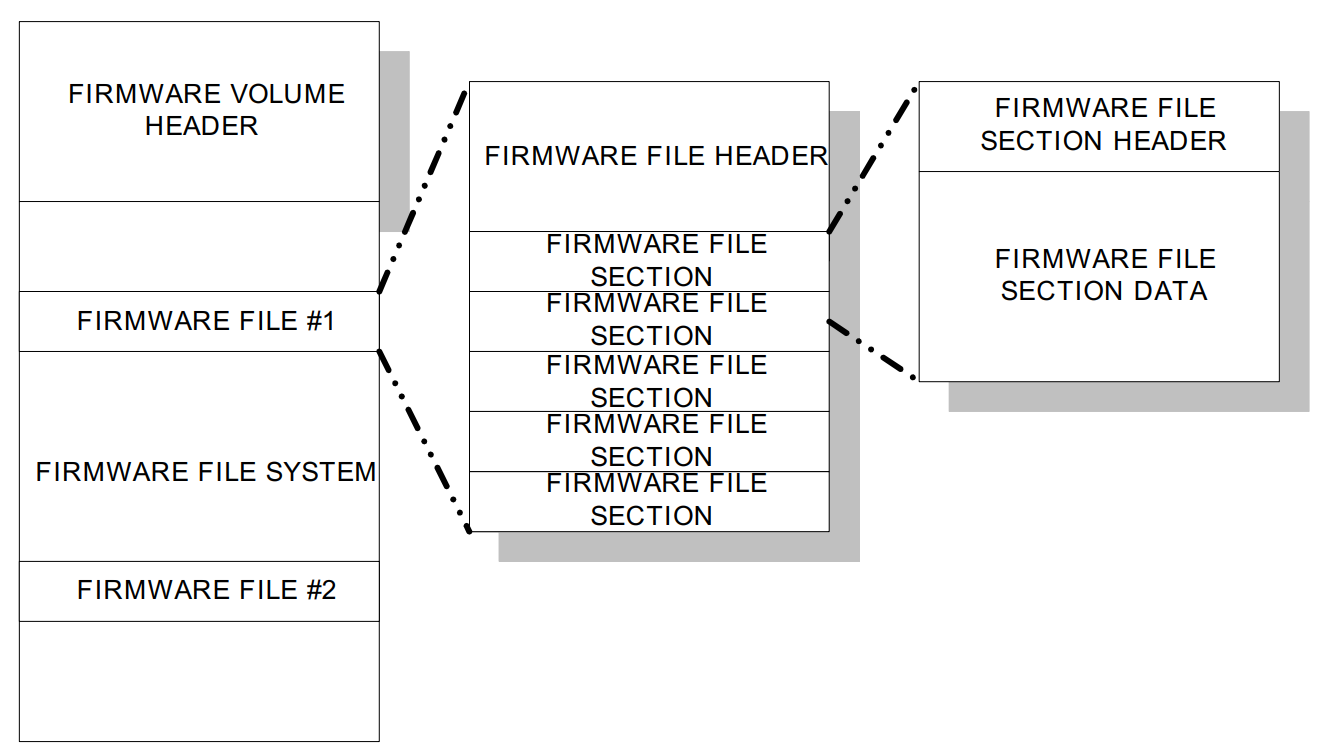
\includegraphics[width=0.8\linewidth]{architecture/the-firmware-volume-format}
	\caption{The Firmware Volume Format}\label{fig:architecture-the-firmware-volume-format}
\end{figure}

The standard firmware volume format (Figure \ref{fig:architecture-the-firmware-volume-format}) consists of two parts: the firmware volume header and the firmware volume data. The firmware volume header describes all of the attributes specified in “Firmware Volumes” on Table \ref{table:firmware-volume-attributes}. The header also contains a GUID which describes the format of the firmware file system used to organize the firmware volume data. The firmware volume header can support other firmware file systems other than the PI Firmware File System.

The PI Firmware File System format describes how firmware files and free space are organized
within the firmware volume.

The PI Firmware File format describes how files are organized. The firmware file format consists of
two parts: the firmware file header and the firmware file data.

\subsubsection{Firmware Volume Format}
he PI Architecture Firmware Volume format describes the binary layout of a firmware volume.
The firmware volume format consists of a header followed by the firmware volume data. The
firmware volume header is described by \verb|EFI_FIRMWARE_VOLUME_HEADER|.
The format of the firmware volume data is described by a GUID. Valid files system GUID values
are \verb|EFI_FIRMWARE_FILE_SYSTEM2_GUID| and \verb|EFI_FIRMWARE_FILE_SYSTEM3_GUID|.

\subsubsection{Firmware File System Format}
The PI Architecture Firmware File System is a binary layout of file storage within firmware
volumes. It is a flat file system in that there is no provision for any directory hierarchy; all files
reside in the root directly. Files are stored end to end without any directory entry to describe which files are present. Parsing the contents of a firmware volume to obtain a listing of files present requires walking the firmware volume from beginning to end.

\paragraph{Firmware File System GUID} The PI Architecture firmware volume header contains a data field for the file system GUID. There are two valid FFS file system, the GUID is defined as \verb|EFI_FIRMWARE_FILE_SYSTEM2_GUID| and \verb|EFI_FIRMWARE_FILE_SYSTEM3_GUID|.
If the FFS file system is backward compatible with \verb|EFI_FIRMWARE_FILE_SYSTEM2_GUID| and supports files larger than $ 16 \ MB $ then \verb|EFI_FIRMWARE_FILE_SYSTEM3_GUID| is used.

\paragraph{Volume Top File} A Volume Top File (VTF) is a file that must be located such that the last byte of the file is also the last byte of the firmware volume. Regardless of the file type, a VTF must have the file name GUID of \verb|EFI_FFS_VOLUME_TOP_FILE_GUID|.
Firmware file system driver code must be aware of this GUID and insert a pad file as necessary to guarantee the VTF is located correctly at the top of the firmware volume on write and update operations. File length and alignment requirements must be consistent with the top of volume. Otherwise, a write error occurs and the firmware volume is not modified.

\subsection{Firmware File Format (\gls{ffs})}
All FFS files begin with a header that is aligned on an $ 8-byte $ boundary with respect to the beginning
of the firmware volume. FFS files can contain the following parts:
\begin{itemize}
	\item Header
	\item Data
\end{itemize}

It is possible to create a file that has only a header and no data, which consumes 24 bytes of space.
This type of file is known as a zero-length file.

If the file contains data, the data immediately follows the header. The format of the data within a file
is defined by the Type field in the header, either \verb|EFI_FFS_FILE_HEADER| or \verb|EFI_FFS_FILE_HEADER2|.

Figure \ref{fig:architecture-typical-ffs-file-layout-less-than-16MB} illustrates the layout of a (typical i.e. \verb|EFI_FFS_FILE_HEADER|) PI Architecture Firmware File smaller than $ 16 Mb $.

\begin{figure}[!htbp]
	\centering
	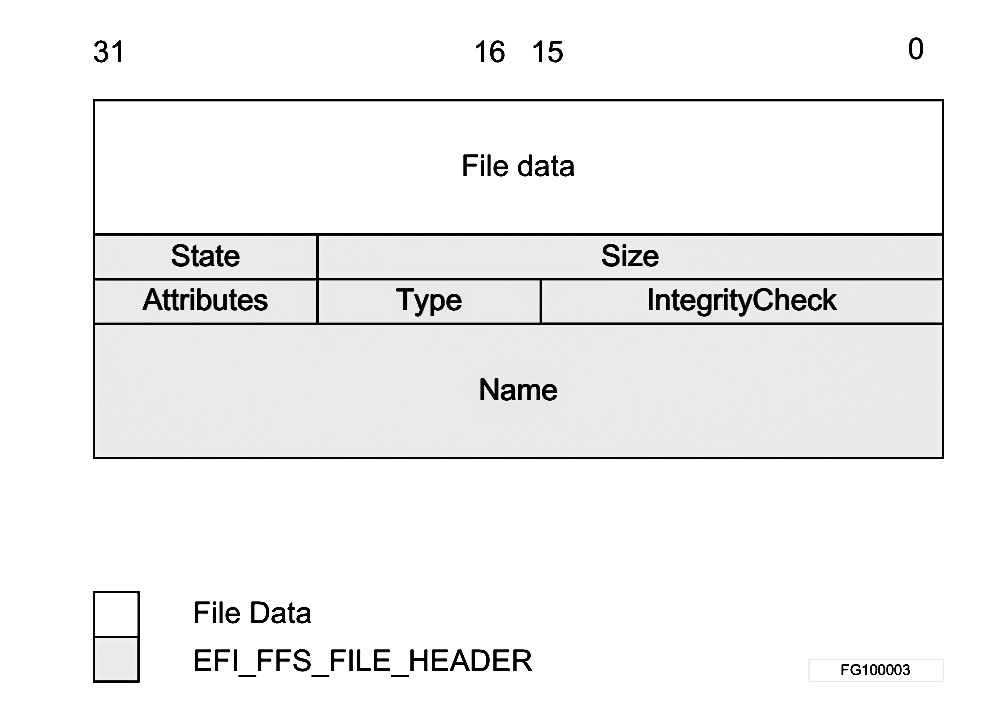
\includegraphics[width=0.8\linewidth]{architecture/typical-ffs-file-layout-less-than-16MB}
	\caption{Typical FFS File Layout}\label{fig:architecture-typical-ffs-file-layout-less-than-16MB}
\end{figure}

Figure \ref{fig:architecture-typical-ffs-file-layout-greater-than-16MB} illustrates the layout of a PI Architecture Firmware File larger than $ 16 Mb $.

\begin{figure}[!htbp]
	\centering
	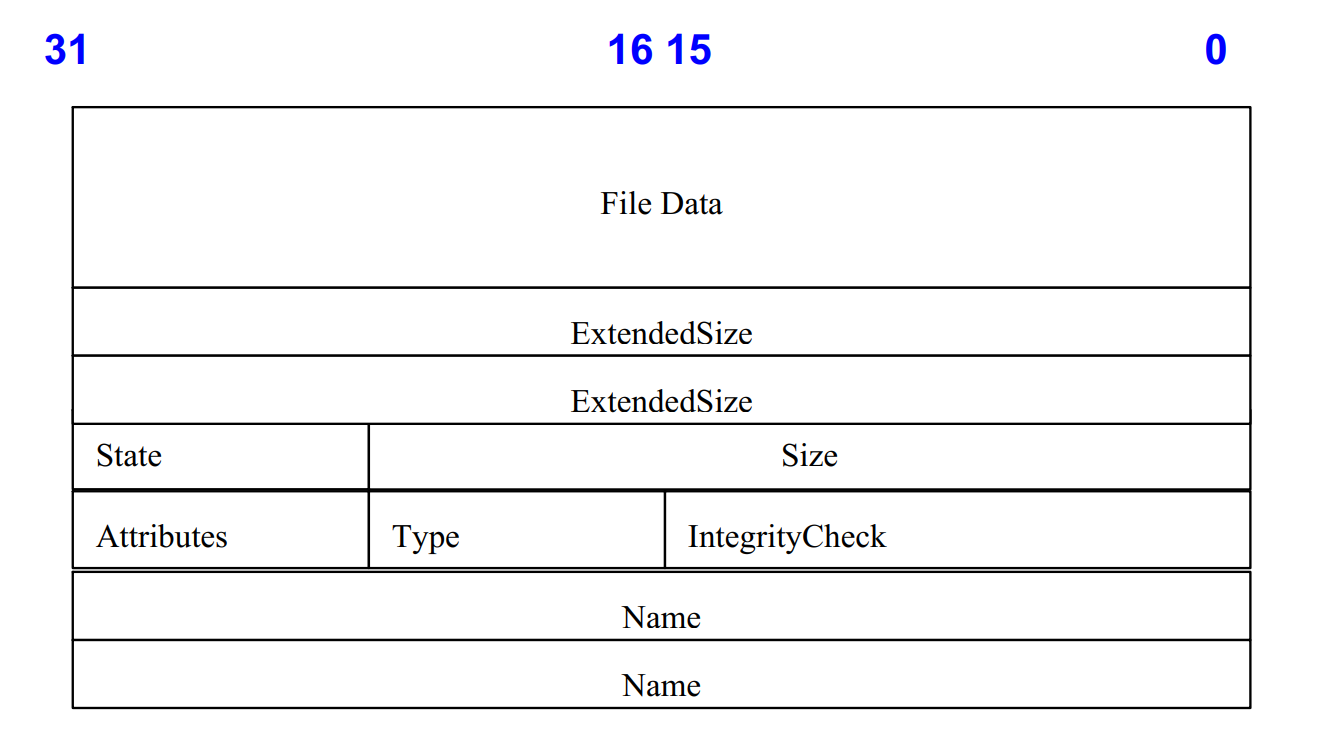
\includegraphics[width=0.8\linewidth]{architecture/typical-ffs-file-layout-greater-than-16MB}
	\caption{File Header 2 layout for files larger than $ 16Mb $}\label{fig:architecture-typical-ffs-file-layout-greater-than-16MB}
\end{figure}


\subsection{Firmware File Section Format}
This section describes the standard firmware file section layout.
Each section begins with a section header, followed by data defined by the section type.
The section headers aligned on 4 byte boundaries relative to the start of the file's image. If padding is
required between the end of one section and the beginning of the next to achieve the 4-byte
alignment requirement, all padding bytes must be initialized to zero.
Many section types are variable in length and are more accurately described as data streams rather
than data structures.

Regardless of section type, all section headers begin with a $ 24-bit $ integer indicating the section size,
followed by an 8-bit section type. The format of the remainder of the section header and the section
data is defined by the section type. If the section size is $ 0xFFFFFF $ then the size is defined by a $ 32-
bit $ integer that follows the $ 32-bit $ section header. Figures \ref{fig:architecture-format-of-a-section-below-16Mb} and \ref{fig:architecture-format-of-a-section-above-16Mb} shows the general format of a section.

\begin{figure}[!htbp]
	\centering
	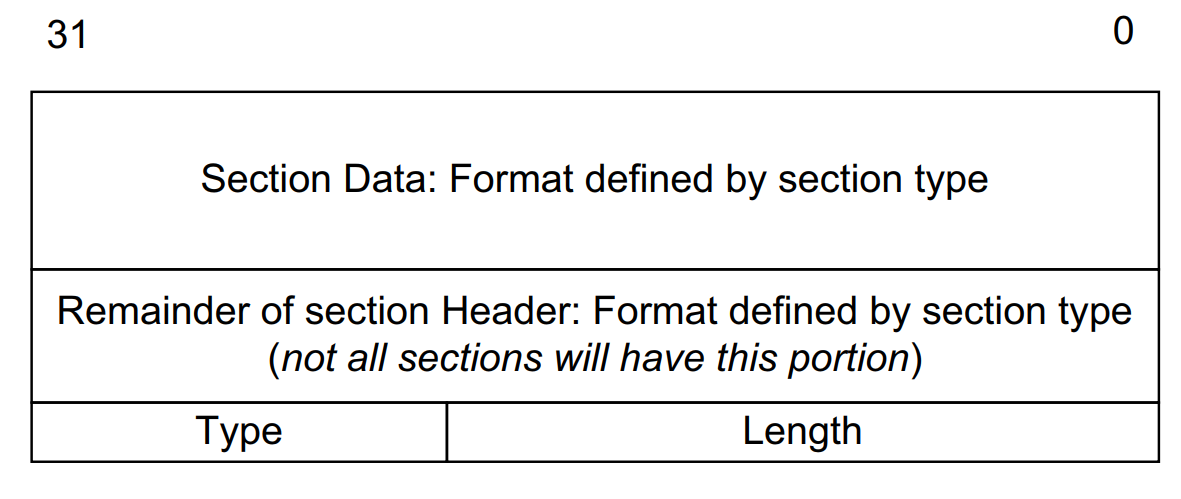
\includegraphics[width=0.8\linewidth]{architecture/format-of-a-section-below-16Mb}
	\caption{Format of a Section below $ 16Mb $}\label{fig:architecture-format-of-a-section-below-16Mb}
\end{figure}

\begin{figure}[!htbp]
	\centering
	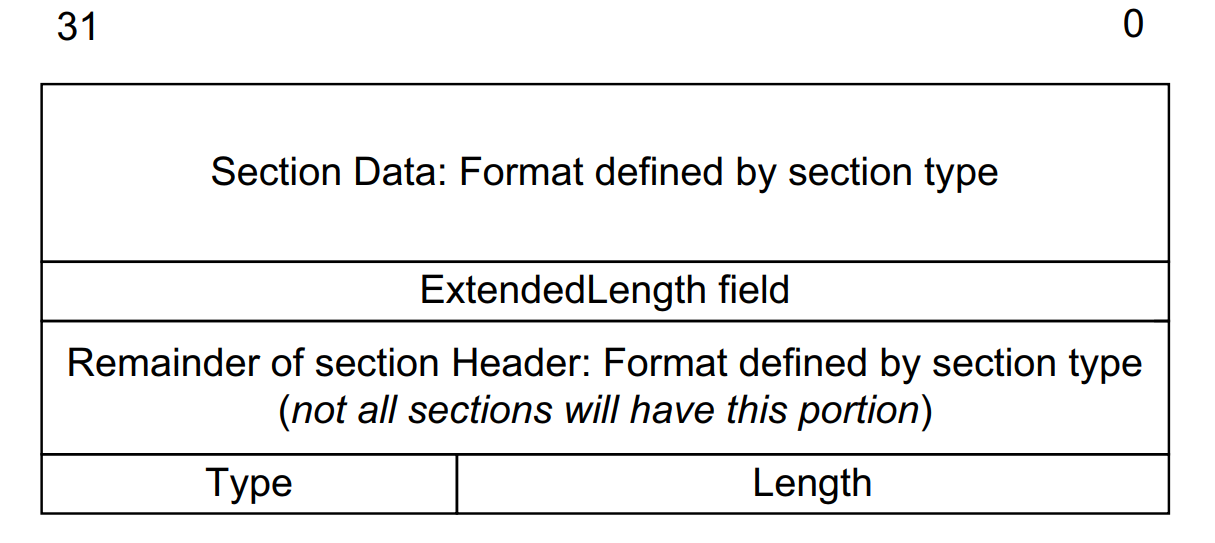
\includegraphics[width=0.8\linewidth]{architecture/format-of-a-section-above-16Mb}
	\caption{Format of a Section using Extended Length field $ 16Mb $}\label{fig:architecture-format-of-a-section-above-16Mb}
\end{figure}


\subsection{File System Initialization}\label{subsection:file-system-initialization}
The algorithm \ref{code:architecture-file-system-initialization} describes a method of FFS initialization that ensures FFS file corruption can be detected regardless of the cause.

The State byte of each file must be correctly managed to ensure the integrity of the file system is
not compromised in the event of a power failure during any FFS operation. It is expected that an FFS
driver will produce an instance of the Firmware Volume Protocol and that all normal file operations
will take place in that context. All file operations must follow all the creation, update, and deletion
rules described in this specification to avoid file system corruption.

The following \verb|FvCheck()| pseudo code must be executed during FFS initialization to avoid file
system corruption. If at any point a failure condition is reached, then the firmware volume is
corrupted and a crisis recovery is initiated.All FFS files, including files of type
\verb|EFI_FV_FILETYPE_FFS_PAD| must be evaluated during file system initialization. It is legal for
multiple pad files with this file type to have the same Name field in the file header. No checks for
duplicate files should be performed on pad files.

\inputminted{c}{code/architecture-file-system-initialization.c}\label{code:architecture-file-system-initialization}

\subsection{Traversal and Access to Files}
The Security (SEC), PEI, and early DXE code must be able to traverse the FFS and read and execute
files before a write-enabled DXE FFS driver is initialized. Because the FFS may have
inconsistencies due to a previous power failure or other system failure, it is necessary to follow a set
of rules to verify the validity of files prior to using them. It is not incumbent on SEC, PEI, or the
early read-only DXE FFS services to make any attempt to recover or modify the file system. If any
situation exists where execution cannot continue due to file system inconsistencies, a recovery boot
is initiated.

There is one inconsistency that the SEC, PEI, and early DXE code can deal with without initiating a
recovery boot. This condition is created by a power failure or other system failure that occurs during
a file update on a previous boot. Such a failure will cause two files with the same file name GUID to
exist within the firmware volume. One of them will have the \verb|EFI_FILE_MARKED_FOR_UPDATE|
bit set in its State field but will be otherwise a completely valid file. The other one may be in any
state of construction up to and including \verb|EFI_FILE_DATA_VALID|. All files used prior to the
initialization of the write-enabled DXE FFS driver must be screened with this test prior to their use.
If this condition is discovered, it is permissible to initiate a recovery boot and allow the recovery
DXE to complete the update.
The following pseudo code describes the method for determining which of these two files to use.
The inconsistency is corrected during the write-enabled initialization of the DXE FFS driver.

\inputminted{c}{code/architecture-traversal-and-file-access.c}\label{code:architecture-traversal-and-file-access}


\paragraph{Note} There is no check for duplicate files once a file in the \verb|EFI_FILE_DATA_VALID| state is located.
The condition where two files in a single firmware volume have the same file name GUID and are
both in the \verb|EFI_FILE_DATA_VALID| state cannot occur if the creation and update rules that are
defined in this specification are followed.

\subsection{File Integrity and State}
File corruption, regardless of the cause, must be detectable so that appropriate file system repair
steps may be taken. File corruption can come from several sources but generally falls into three
categories:
\begin{itemize}
	\item General failure
	\item Erase failure
	\item Write failure
\end{itemize}

A general failure is defined to be apparently random corruption of the storage media. This
corruption can be caused by storage media design problems or storage media degradation, for
example. This type of failure can be as subtle as changing a single bit within the contents of a file.
With good system design and reliable storage media, general failures should not happen. Even so,
the FFS enables detection of this type of failure.

An erase failure occurs when a block erase of firmware volume media is not completed due to a
power failure or other system failure. While the erase operation is not defined, it is expected that
most implementations of FFS that allow file write and delete operations will also implement a
mechanism to reclaim deleted files and coalesce free space. If this operation is not completed
correctly, the file system can be left in an inconsistent state.
Similarly, a write failure occurs when a file system write is in progress and is not completed due to a
power failure or other system failure. This type of failure can leave the file system in an inconsistent
state.

All of these failures are detectable during FFS initialization, and, depending on the nature of the
failure, many recovery strategies are possible. Careful sequencing of the State bits during normal
file transitions is sufficient to enable subsequent detection of write failures. However, the State
bits alone are not sufficient to detect all occurrences of general and/or erase failures. These types of
failures require additional support, which is enabled with the file header \verb|IntegrityCheck| field.
For sample code that provides a method of FFS initialization that can detect FFS file corruption,
regardless of the cause, see “File System Initialization” on Section \ref{subsection:file-system-initialization}.




\section{System Management Mode (\gls{smm})}\label{section-smm}
\subsection{Overview}
On \say{IA-32 processors}, System Management Mode (\gls{smm}) is a manner of operation which is different from flat modal so as from protected mode of the DXE and PEI phases. It is outlined as a real mode environs with $ 32-bit $ data bus access and its carried out in effect to either with a specified interrupt type or with the System Management Interrupt (\gls{smi}) pin. Note that Operation mode of SMM is OS independent mode and is discrete operational mode, however it may also lies in both within and OS runtime.

\begin{figure}[!htbp]
	\centering
	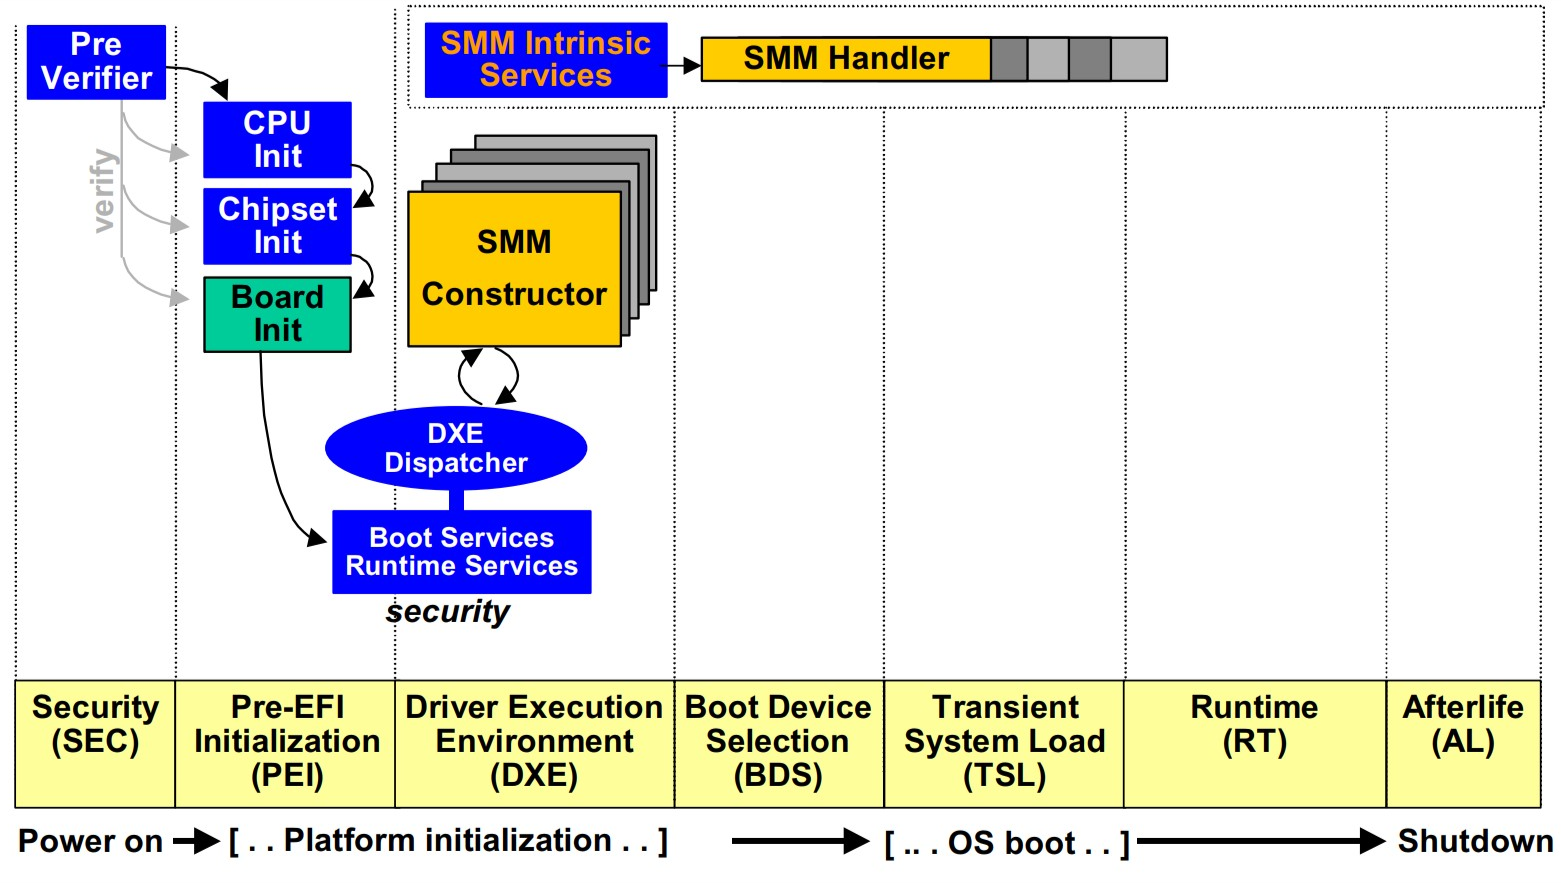
\includegraphics[width=0.9\linewidth]{smm/framework-smm-architecture}
	\caption{SMM Framework Architecture}\label{fig:framework-smm-architecture}
\end{figure}


\subsection{System Management System Table (\gls{smst})}
System Management System Table (\gls{smst}) is core mechanism of SMM handler to pass information and enabling activity.

SMST table allows access to service based on the SMST which also known as SMM Services. Driver can only use SMM services during execution inside context of the SMM. \verb|EFI_SMM_BASE_PROTOCOL.GetSmstLocation()| service used to discover the address of SMST.

SMST is a set of potentiality exported for utilization by any driver that is loaded into \gls{smram}. It's similar to the EFI System Table except that by design it's fixed set of services and data and also doesn't acknowledge to the resiliency of an EFI protocol interface.

SMM infrastructure component of Framework provides SMST, which manages:
\begin{itemize}
	\item Dispatching drivers inside SMM
	\item Allocation of memory (\gls{smram})
	\item Switching the framework in and out of the applicable SMM of the processor
\end{itemize}

\subsection{SMM and Available Services}\label{subsection-smm-available-services}

\subsubsection{SMM Services}\label{subsection-smm-services}
As EFI runtime drivers have their constraints, similarly the model of SMM  framework will have them too. Especially, dispatch of drivers in SMM won't be capable of using any core protocol service. However SMST-based services, called SMM Services allows the drivers to be access using an SMM identical of the EFI System Table, but services of the core protocol won't grantees the availability in runtime. As an alternative, the complete mass of EFI Boot Services and EFI Runtime Services can be available while the driver loading or "constructor" phase. 

With utilizing the visibility of constructor, SMM driver is capable to leveraging rich set of EFI service to perform:
\begin{itemize}
	\item Marshall interface for EFI services.
	\item Observing EFI protocols which are populated by other SMM drivers while in constructor phase.
\end{itemize}

For drivers while not in SMM and during the initial load inside SMM, EFI protocol database becomes quite useful by utilizing design.

Available services which are SMST-based includes:
\begin{itemize}
	\item Negligible, blocking kind of the device Input/Output protocol
	\item Memory allocator from SMRAM
\end{itemize}
These services are exposed through the entries present in the System Management System Table (SMST).

\subsubsection{SMM Library}\label{subsection-smm-lib}
During constructor phase of SMM driver inside SMM, all additional service within SMM Library (SMLib) are uncovered like EFI protocols. i.e., An identical status code in SMM is merely an EFI protocol with interface referencing an SMM-based driver service. To avoid error or information of progress during runtime, other SMM drivers also locates this SMM based status code.

\subsection{SMM Drivers}\label{subsection-smm-drivers}
\subsubsection{Process to Load Drivers in SMM}
Process to load driver modal in SMM is merely a DXE SMM runtime driver having a DEPEX (dependency expression) having at least \verb|EFI_SMM_BASE_PROTOCOL|. This kind of dependency is essential as the DXE runtime driver which is planned for SMM will utilize the \verb|EFI_SMM_BASE_PROTOCOL| to load up itself again in SMM and re-execute its entry point. Also, other SMM-loaded protocols permitted to be stayed in the DEPEX of specified SMM DXE runtime driver. Principle of the DXE Dispatcher is to verifying if the GUIDs to be consumed by the protocols does exists in the database of protocol and capable to identifying if the driver can be loaded or not.

After formerly loaded in SMM the DXE SMM runtime driver becomes capable utilize only minor set of services. While in its constructor entry point, the driver can use EFI Boot Services as it executes within space of boot service and SMM.

In secondary entry point in SMM driver is capable to perform:
\begin{itemize}
	\item Registration of an interface - In the formal protocol database, naming the SMM occupant interfaces with future-loaded SMM drivers
	\item Registration with the SMM codebase - For a callback hook in effect to an SMI pin stimulation or an SMI based interrupt message from outside of SMM Code (i.e. a boot service, runtime agent)
\end{itemize}

After this \textbf{constructor} phase in SMM, the SMM driver needs not be rely on any other boot services as the mode of operation to carrying out execution can move away from these services. Many EFI Runtime Services could possess the majority of their execution shifted into SMM and viewable runtime portion simply becomes a proxy which merely utilizes the \verb|EFI_SMM_BASE_PROTOCOL| to perform callback in SMM to carry out services. By Possessing a proxy which allows for a modal of sharing code blocks of error handling, like services for flash access and also the EFI Runtime Services \verb|GetVariable()| or \verb|SetVariable()|.

\subsubsection{SMM Drivers for IA-32}
In SMM the \say{IA-32 runtime drivers} can not called as on the image the action by \verb|SetVirtualAddress()| is performed. Hence, code segment that requires to be accessible among SMM and EFI runtime needs to be migrated in SMM.

\subsubsection{"Itanium® Processor Family" SMM Drivers}
From \say{Platform Management Interrupt (\gls{pmi})} the runtime drivers for the \say{Itanium® processor family} are called as if each of them is kind of \say{Position Independent Code (PIC) runtime driver}.

\subsection{SMM Protocols}\label{subsection-smm-protocols}
System Architecture of SMM broke in to below two parts:
\begin{itemize}
	\item \say{SMM Base Protocol} - exposed by the processor. This protocol is liable to perform: 
		\begin{itemize}
			\item To initialize the state of processor
			\item Registration of the handlers
		\end{itemize}
	\item \say{SMM Access Protocol} - interprets the specific enabling and locking mechanism that an IA-32 memory controller may allows during execution in SMM. (Not needed for \say{Itanium® processor family})
\end{itemize}

\subsubsection{SMM Protocols for IA-32}
Figure \ref{fig:published-protocols-for-ia-32-systems} shows the SMM protocols which are published for an IA-32 system.
\begin{figure}[!htbp]
	\centering
	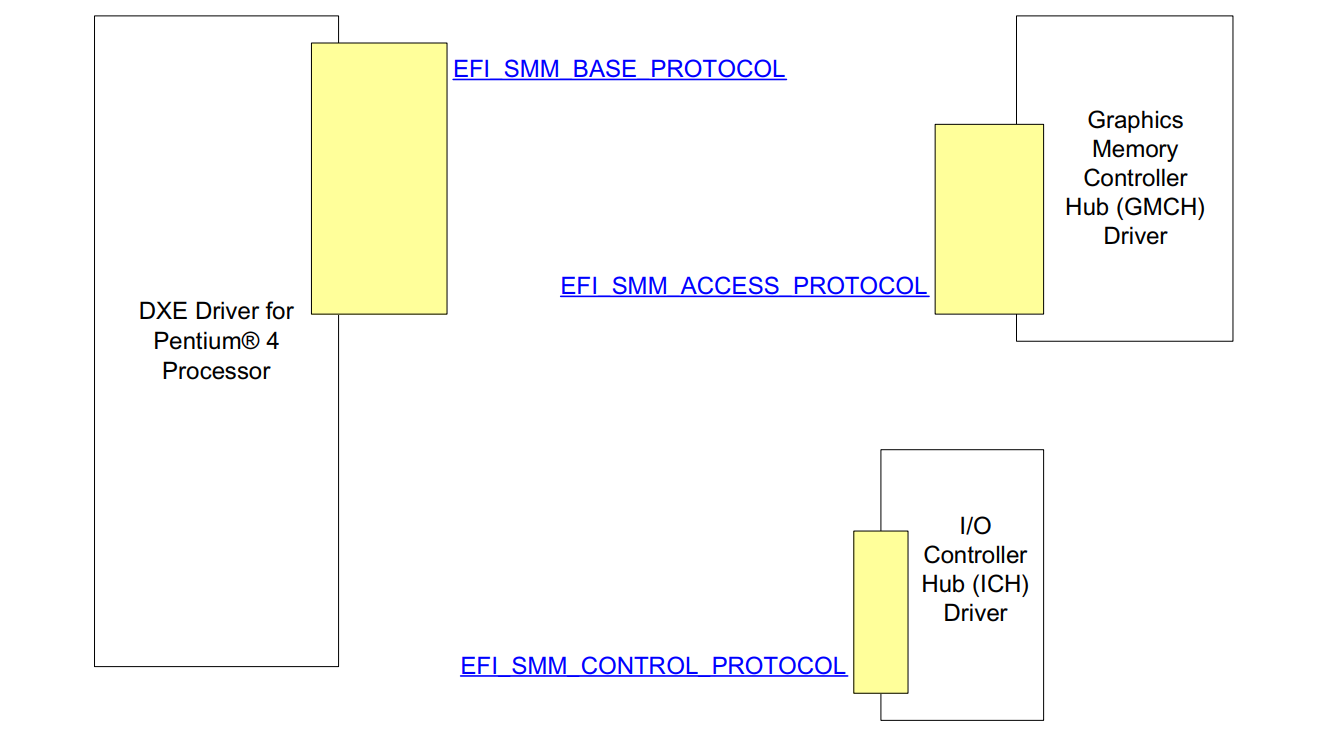
\includegraphics[width=0.9\linewidth]{smm/published-protocols-for-ia-32-systems}
	\caption{Protocols Published for IA-32 Systems}\label{fig:published-protocols-for-ia-32-systems}
\end{figure}

\subsubsection{SMM Protocols for "Itanium®-Based Systems"}
Figure \ref{fig:published-protocols-for-itanium-systems} shows the way SMM protocols are published for an \say{Itanium®-Based system}.
\begin{figure}[!htbp]
	\centering
	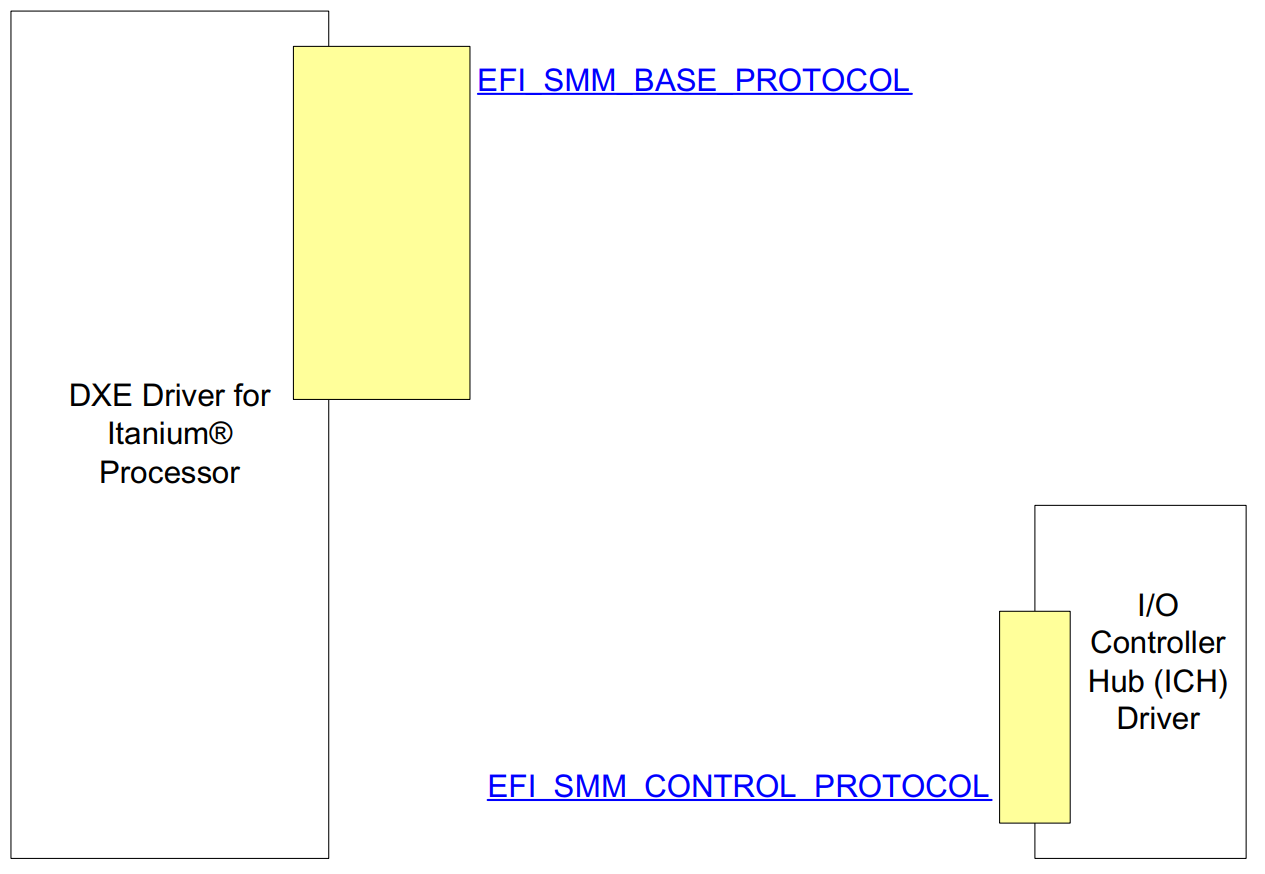
\includegraphics[width=0.9\linewidth]{smm/published-protocols-for-itanium-systems}
	\caption{Protocols Published for "Itanium®-Based Systems"}\label{fig:published-protocols-for-itanium-systems}
\end{figure}


\subsection{SMM Dispatcher and infrastructure}
SMM Code segment lies within the SMM Dispatcher. Major Role of SMM Dispatcher is to give the control mode to the SMM handlers in a systematic methodology. SMM Infrastructure Code aids to drive communication for SMM to SMM. SMM handlers are PE32+ images.

\subsection{Initializing SMM Phase}
The SMM driver for the Framework is fundamentally a enrollment transport mode to dispatch the drivers in outcome to the:
\begin{itemize}
	\item System Management Interrupts for \say{IA-32}
	\item Platform Management Interrupts (PMIs) for \say{Itanium® processor family}
\end{itemize}

\subsection{Relation of "System Management RAM (\gls{smram})" to conventional memory}
Figure \ref{fig:smram-relationship-to-main-memory} shows relationship between SMRAM and main memory in IA-32. Where SMRAM is isolated secure part inside the conventional main memory.

\begin{figure}[!htbp]
	\centering
	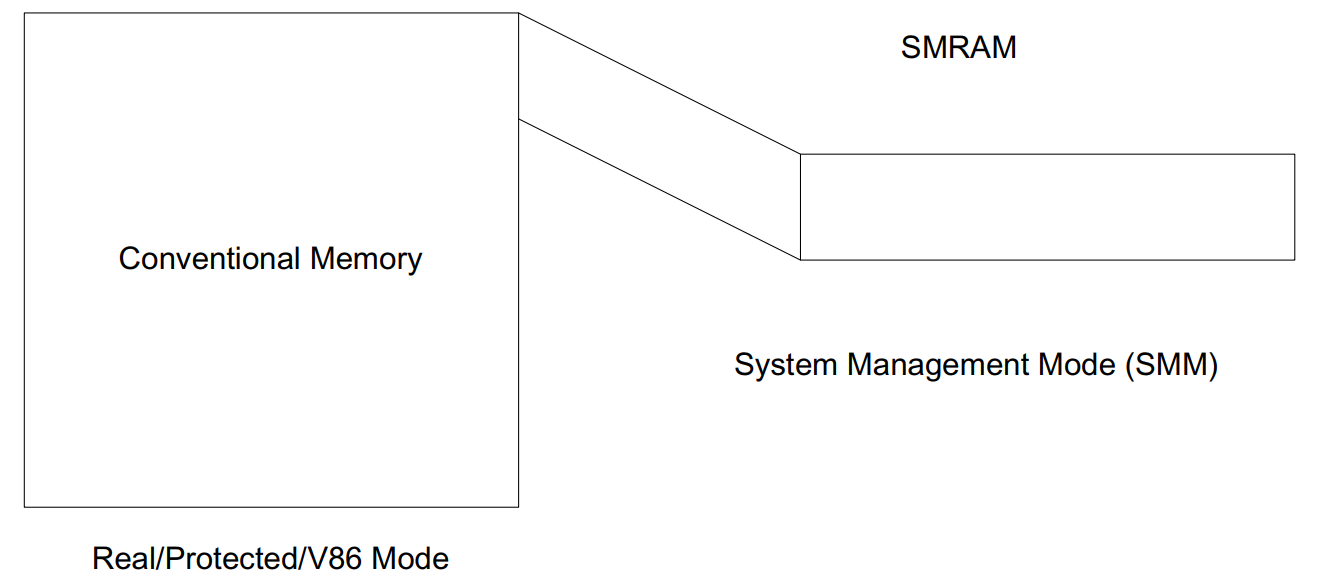
\includegraphics[width=0.9\linewidth]{smm/smram-relationship-to-main-memory}
	\caption{SMRAM kinship with conventional memory}\label{fig:smram-relationship-to-main-memory}
\end{figure}

\subsection{Execution Mode of SMM on Processor}\label{subsection-processor-execution-mode}
SMM is acceded asynchronously with the ongoing main flow of program. SMM was primitively developed to be clear to the OS and provide a power management facility more transparent.

Preboot agents are responsible to initiate alternate uses of SMM which are:
\begin{itemize}
	\item Applicable Workaround for \gls{soc} exaggeration
	\item Logging of error(s)
	\item Security for the platform
\end{itemize}

A \gls{smi} can be launched by energizing either the SMI logic pin via dedicated on the board or by utilizing the local APIC.

\say{Itanium® architecture} possess no independent separate mode for processor for the tractability of interruption however it does supports \say{Platform Management Interrupt (\gls{pmi})} which indeed is a maskable interruption. However, there is this another way to enter PMI using a interrupt message on local \say{Streamlined Advanced Programmable Interrupt Controller (\gls{sapic})}.

This architecture informs a techniques to load modules of needful code segment that substantiate the functionality specified above. The internal representation of protocol which enables the loading of images of various handler and runs in normal memory of boot-services. Only the handlers does to run in \gls{smram}.

\subsection{Accessing Platform Resources}\label{subsection-access-to-platform-resources}
As par policy outcome process of the execution of SMM handlers is reasonably prevents from accessing conventional memory resources. Hence, there does not exist any ease binding technique such as a call or trap interface to render the services in preemptive bid of non-SMM state.

Besides, SMM Services - the library of service which abides a sub set of the core EFI services, i.e. device input-output protocol, memory allocation and others. Also, execution mode of SMM driver has the equivalent structure as per the EFI criterion - namely a components which executes under boot services and it could perhaps run in runtime mode. When \verb|ExitBootServices()| invoked, the mechanism of an unregister event occurs.




\chapter{Implementation}\label{chapter-implementation}
\lhead{Chapter 3. \emph{Implementation}}

\section{Proposed Work}\label{section-proposed-work}
In general to generate BIOS image (*.rom file), compilation of XYZ.c (source code) has to be done, this compilation not only involves compilation of DXE driver, PEI driver, EFI Application but also includes pre-processing checks, compression of raw files which takes huge amount of time depending on the system configuration. Implementation of this project aids in reduction of this compilation time.

\subsection{Stake holders}\label{subsection-stack-holders}
The proposed work is applicable but not limited to below stake holders:
\begin{itemize}
	\item \textbf{BIOS development team} : main development group in contributing BIOS firmware, this is the only stake holder who are having access to the BIOS development environment and access to the source code of the complete BIOS firmware
	\item \textbf{Validation team} : performs various validation on developed BIOS image
	\item \textbf{Automation team} : brings various integration and validation automation to module(s)
	\item Other Development team who wishes to ease the debugging process
\end{itemize}

\subsection{Issues}\label{subsection-issues}
The Proposed work is capable of mitigating below issues:
\begin{itemize}
	\item Generation of BIOS image - includes compilation of whole source code
	\item Time complexity - took enormous amount of time to generate the BIOS image
	\item Accessing and modifying BIOS Setup Option(s) remotely
	\item Firmware Flashing of BIOS remotely
	\item Updating CPU microcode
	\item Summarizing changes among BIOS image
	\item Avoiding exposing the source code support for OEM to fill their OEM information
	\item Avoid setting of BIOS development platform for stake holders which are not meant to be the BIOS developer
	\item Runtime BIOS Support for temporary UEFI variable creation
\end{itemize}

\subsection{Requirements}\label{subsection-requirements}
\subsubsection{Software Requirements}
\begin{itemize}
	\item Visual C/C++ binaries
	\item Python 3
	\item Visual Studio Code (IDE)
	\item Memory Access Interface - supported mechanism to communicate over target memory
\end{itemize}

\subsection{Development Process of Modules}
Framework development process is driven by implementation of independent modules which can serve functionality and having flexibility to integration to the framework.


% ========================================================================
% MODULE 1
% ========================================================================

%\subsection{Module 1: Processing Firmware individually}\label{subsection-processing-firmware}
%To process apply the whole firmware changes individually for BIOS, signing is require to be performed for individual Firmware before stitching it to the BIOS binary in the valid structure.
%
%\subsubsection{Primary Goals of the module}
%\begin{itemize}
%	\item Remove other Intellectual Property's dependency (\gls{ip} dependency) during firmware loading
%	\item \gls{ip} Subsystem :
%	\begin{itemize}
%		\item Loader and Verifier
%		\item \gls{ip} is always consumer
%	\end{itemize}
%	\item Signature verification using \gls{sha} hash algorithm and should be ease support for adding new algorithmic support as needed.
%	\item Should support hardware based and software based verification support
%	modifying memory requirements for given IP without impacting eco-system
%	\item Prevent common security threats
%	\item Allow easier OEM adoption and modification based on the respective design
%	\item Reusability/Portability of design across many \gls{ip}s
%	\item Generic design which supports any new IP integration
%\end{itemize}
%
%\begin{figure}[!htbp]
%	\centering
%	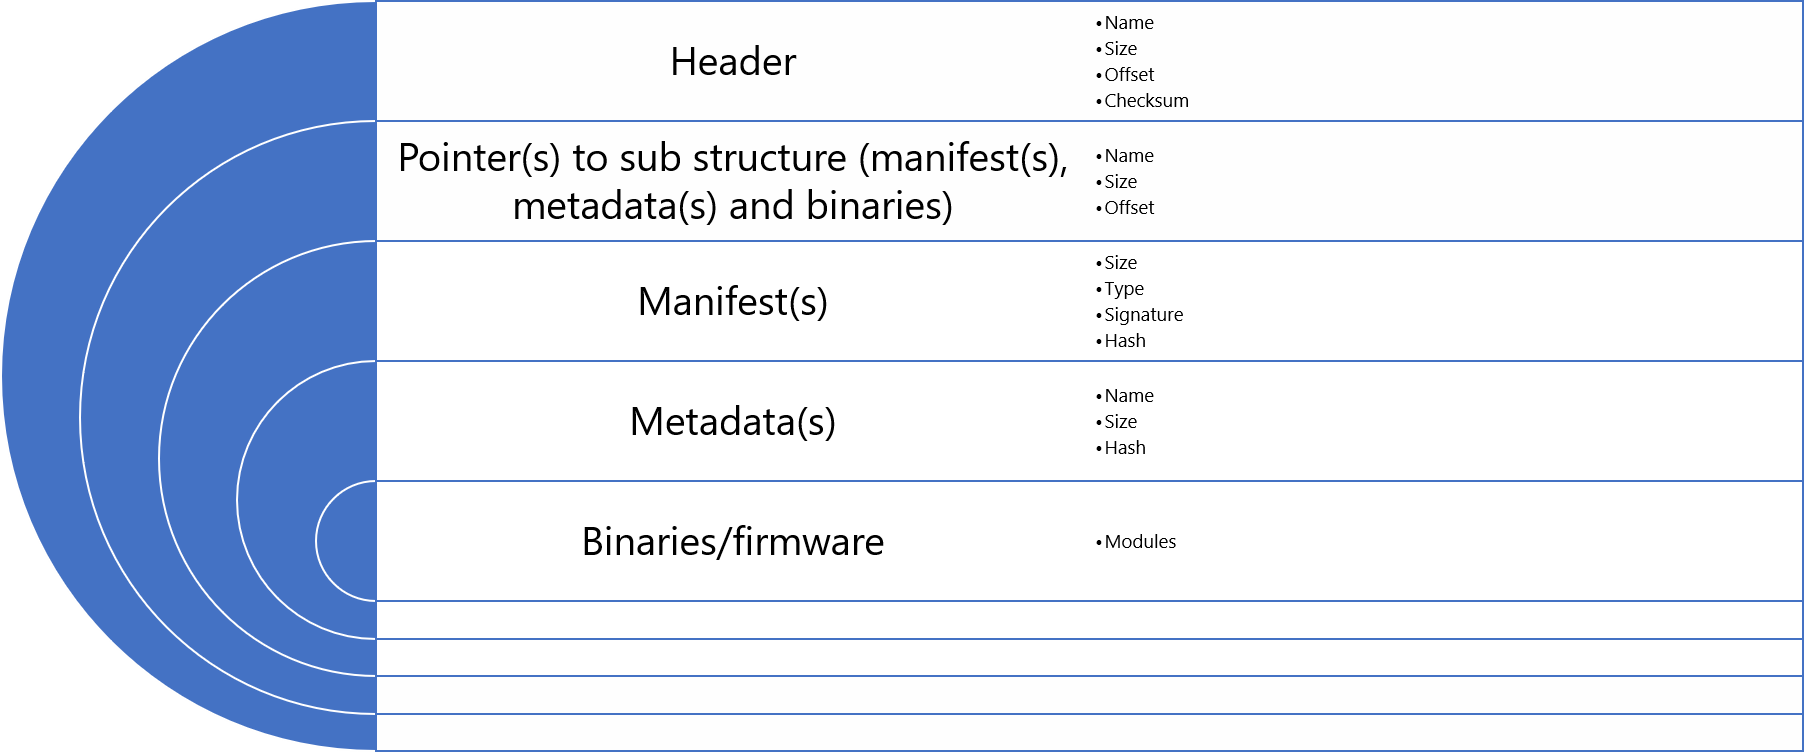
\includegraphics[width=\linewidth]{proposed-work/proposed-structure-firmware-signing}
%	\caption{Proposed Structure for firmware signing}\label{fig:proposed-work-proposed-structure-firmware-signing}
%\end{figure}
%
%Note: Due to Confidentiality other details of this module is not to be disclosed such as flow diagram, structures or pseudo code.

% ========================================================================
% MODULE 1
% ========================================================================
\subsection{Module: Setup Knob modification}\label{module-setup-knob-modification}

\subsubsection{Processing Unsigned debug BIOS}\label{subsection-processing-bios}
Before Releasing the BIOS firmware for public use, those are signed for security and integrity purpose, however the debug BIOS which are used Pre-release to test and verify all the functional features until all the requirements are met.

Every \gls{soc} system which are under test known is \gls{sut} are configured in such a way that it supports debug BIOS. The proposed framework is designed to simulate the process of \gls{sut} in terms of processing BIOS binary similar to \gls{sut} performs it after flashing BIOS firmware on \gls{soc}.

Processing the debug BIOS can be classified in to two ways:
\begin{enumerate}\label{cli-classification-proposed-work}
	\item Applying changes directly to the \gls{sut}
	\item Applying changes on to the BIOS image
\end{enumerate}

At the high level the flow for both the above classification remains the same but will be differentiated at the backend support. An additional driver is attached with BIOS firmware to aid the framework to be able to apply changes directly to the \gls{sut}.

\subsubsection{Additional Tech Stack Used}
Below are the listed technologies consumed in development of this module in addition to the already specified requirements in Section \ref{subsection-requirements}
\begin{itemize}
	\item Tkinter
	\item XML
	\item JSON
\end{itemize}

\subsubsection{Flow of the module}
Figure \ref{fig:setup-knobs-flow} describes the flow of setup knobs modification on the System Under Test (SUT).

\begin{figure}[!htbp]
	\centering
	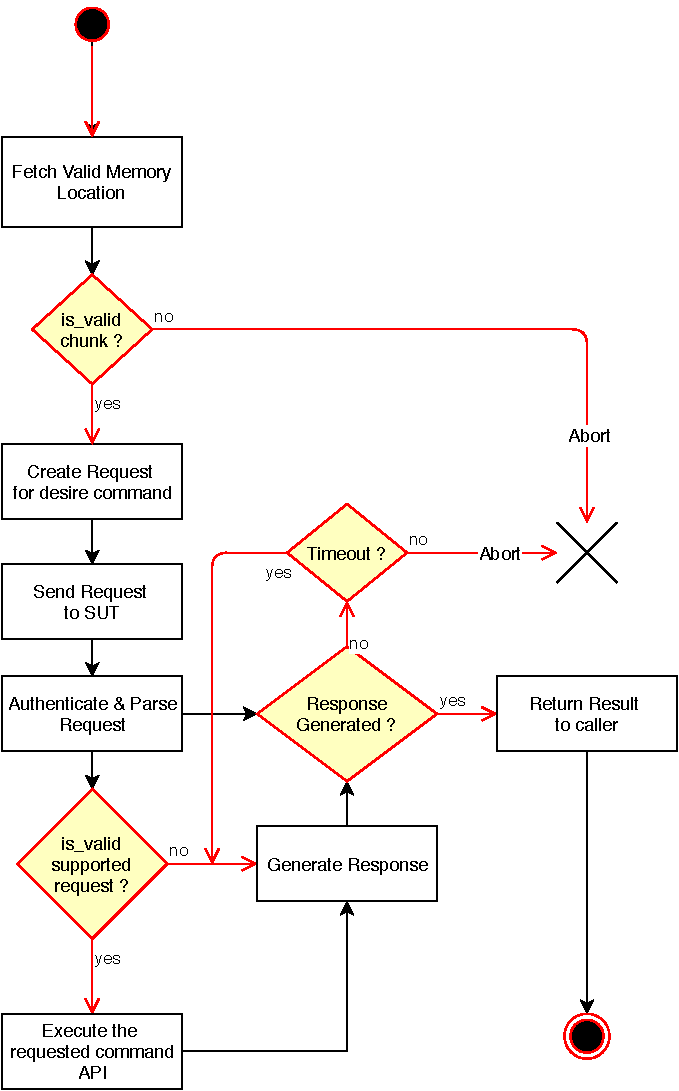
\includegraphics[width=0.9\linewidth]{proposed-work/setup-knobs-flow}
	\caption{Flow of Setup Knobs Modification}\label{fig:setup-knobs-flow}
\end{figure}


\subsubsection{Screenshots of Module}
As a \gls{poc} for the framework, this section shows snapshots of the working module to mimic the setup options of BIOS, however as a simulation framework, it also provides quite more features which are not available in the actual BIOS due to memory limitation.

Figure \ref{fig:proposed-work-bios-gui-initial-config} shows the prompt asked to user to select basic configurations before launching the module of framework. Configurations available to select are:

\begin{itemize}
	\item Working Mode (options to be selected as in figure \ref{fig:proposed-work-bios-gui-initial-config-select-mode})
	\begin{itemize}
		\item \verb|online| - to work on \gls{sut} and require to select valid access method for online mode from menu
		\item \verb|offline| - to work on BIOS binary
	\end{itemize}
	\item Access Method - selecting valid access method for working on \gls{sut}
	\item Publish all? - Boolean options to decide whether to evaluate \gls{depex} or not.
\end{itemize}

\begin{figure}[!htbp]
	\centering
	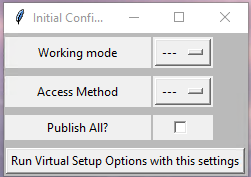
\includegraphics[width=0.7\linewidth]{proposed-work/bios-gui-initial-config}
	\caption{Menu to Select initial configuration for work}\label{fig:proposed-work-bios-gui-initial-config}
\end{figure}

\begin{figure}[!htbp]
	\centering
	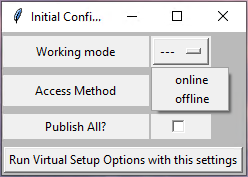
\includegraphics[width=0.7\linewidth]{proposed-work/bios-gui-initial-config-select-mode}
	\caption{Available work mode for the system: Online and Offline}\label{fig:proposed-work-bios-gui-initial-config-select-mode}
\end{figure}


%Figure \ref{fig:proposed-work-bios-gui-acpi-knobs} shows the view that how an options in the module simulation is loaded.

\begin{table}
	\centering
	\renewcommand{\arraystretch}{2}
	\caption{Interpretation of buttons on Virtual Setup Page GUI}\label{table:interpretation-of-buttons-in-module}
	\begin{tabular}{l | p {8cm}}
		Button & Interpretation
		\\ \hline \hline
		Push Changes & Apply changes to system if online mode else apply changes to `bin` file
		\\ \hline View Changes & View saved changes in new window
		\\ \hline Exit & Exit the GUI
		\\ \hline Reload & Reload the GUI
		\\ \hline Discard Changes & Discard any change made, any value if modified are restored to current value
		\\ \hline Load Defaults & Restore to default values and revert any changes made
		\\ \hline
	\end{tabular}
\end{table}

%\begin{figure}[!htbp]
%	\centering
%	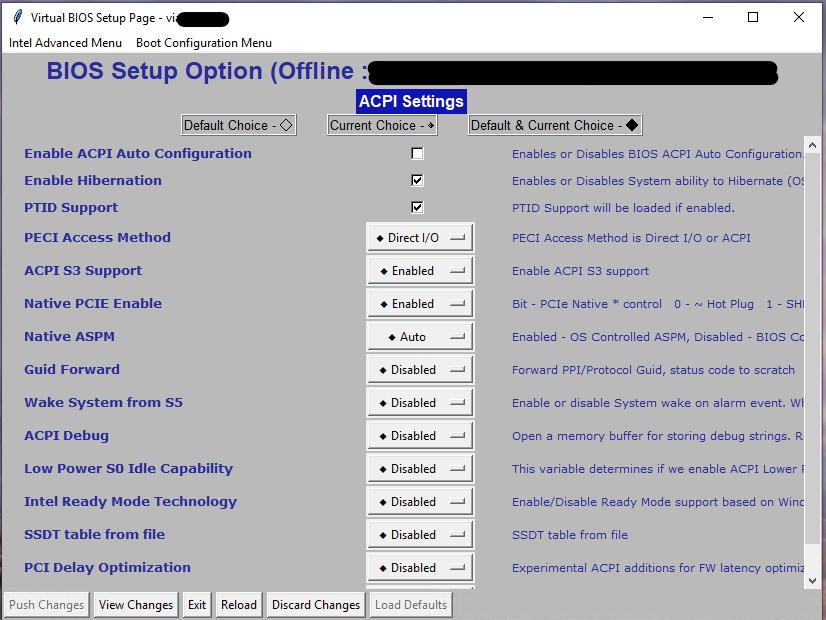
\includegraphics[width=0.8\linewidth]{proposed-work/bios-gui-acpi-knobs}
%	\caption{Setup Options listed under ACPI Configurations}\label{fig:proposed-work-bios-gui-acpi-knobs}
%\end{figure}

Table \ref{table:interpretation-of-buttons-in-module} describes the interpretation of each button action on specific condition as remarks if applicable


%Navigation through the various BIOS pages can be done as shown in Figure \ref{fig:proposed-work-bios-gui-accessing-menu}.

%\begin{figure}[!htbp]
%	\centering
%	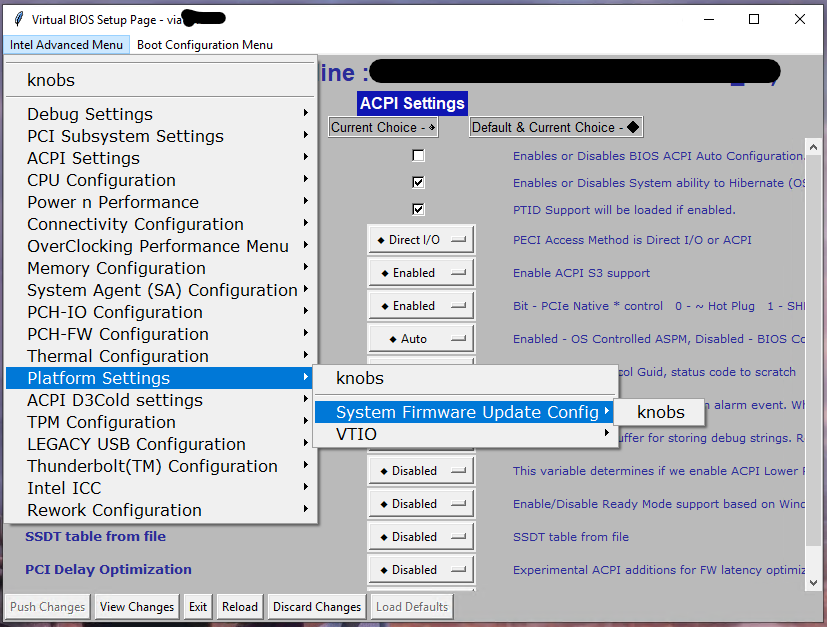
\includegraphics[width=0.8\linewidth]{proposed-work/bios-gui-accessing-menu}
%	\caption{Navigating through BIOS setup page}\label{fig:proposed-work-bios-gui-accessing-menu}
%\end{figure}

%Figure \ref{fig:proposed-work-bios-gui-view-changes} displays list of changes made in setup options across any setup page and listed separately to compare with previous value, discard or apply the new values.

%\begin{figure}[!htbp]
%	\centering
%	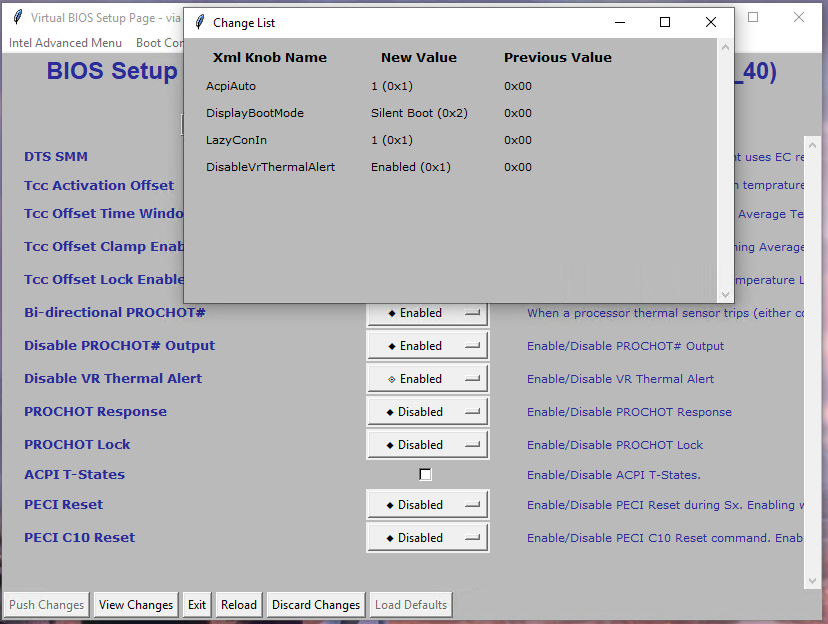
\includegraphics[width=\linewidth]{proposed-work/bios-gui-view-changes}
%	\caption{Viewing all the changes made during current session}\label{fig:proposed-work-bios-gui-view-changes}
%\end{figure}

\subsubsection{Outcome of Module}
\begin{itemize}
	\item The module is capable of cross platform usage.
	\item The module can work with all the platform binary and \gls{sut}.
	\item A communication bridge as a driver in BIOS firmware to aid the framework run directly on \gls{sut} is implemented.
	\item Generic solution is provided for end-user while running any of the classification listed in \ref{cli-classification-proposed-work}.
	\item Simulating the information from system or binary image is provided as native GUI application.
	\item Real time sync with simulation framework is supported.
	\item Seamless Integration of any new features or modules in framework is made possible.
\end{itemize}

% ========================================================================
% MODULE 2
% ========================================================================
\subsection{Module: Parsing}\label{module-parsing}
Figure \ref{fig:bios-as-filesystem} represents the overview of the BIOS as a File system  which is interpreted and parsed from the BIOS image. Detail architecture of the same is explained in Section \ref{section-architecture}

\begin{figure}[!htbp]
	\centering
	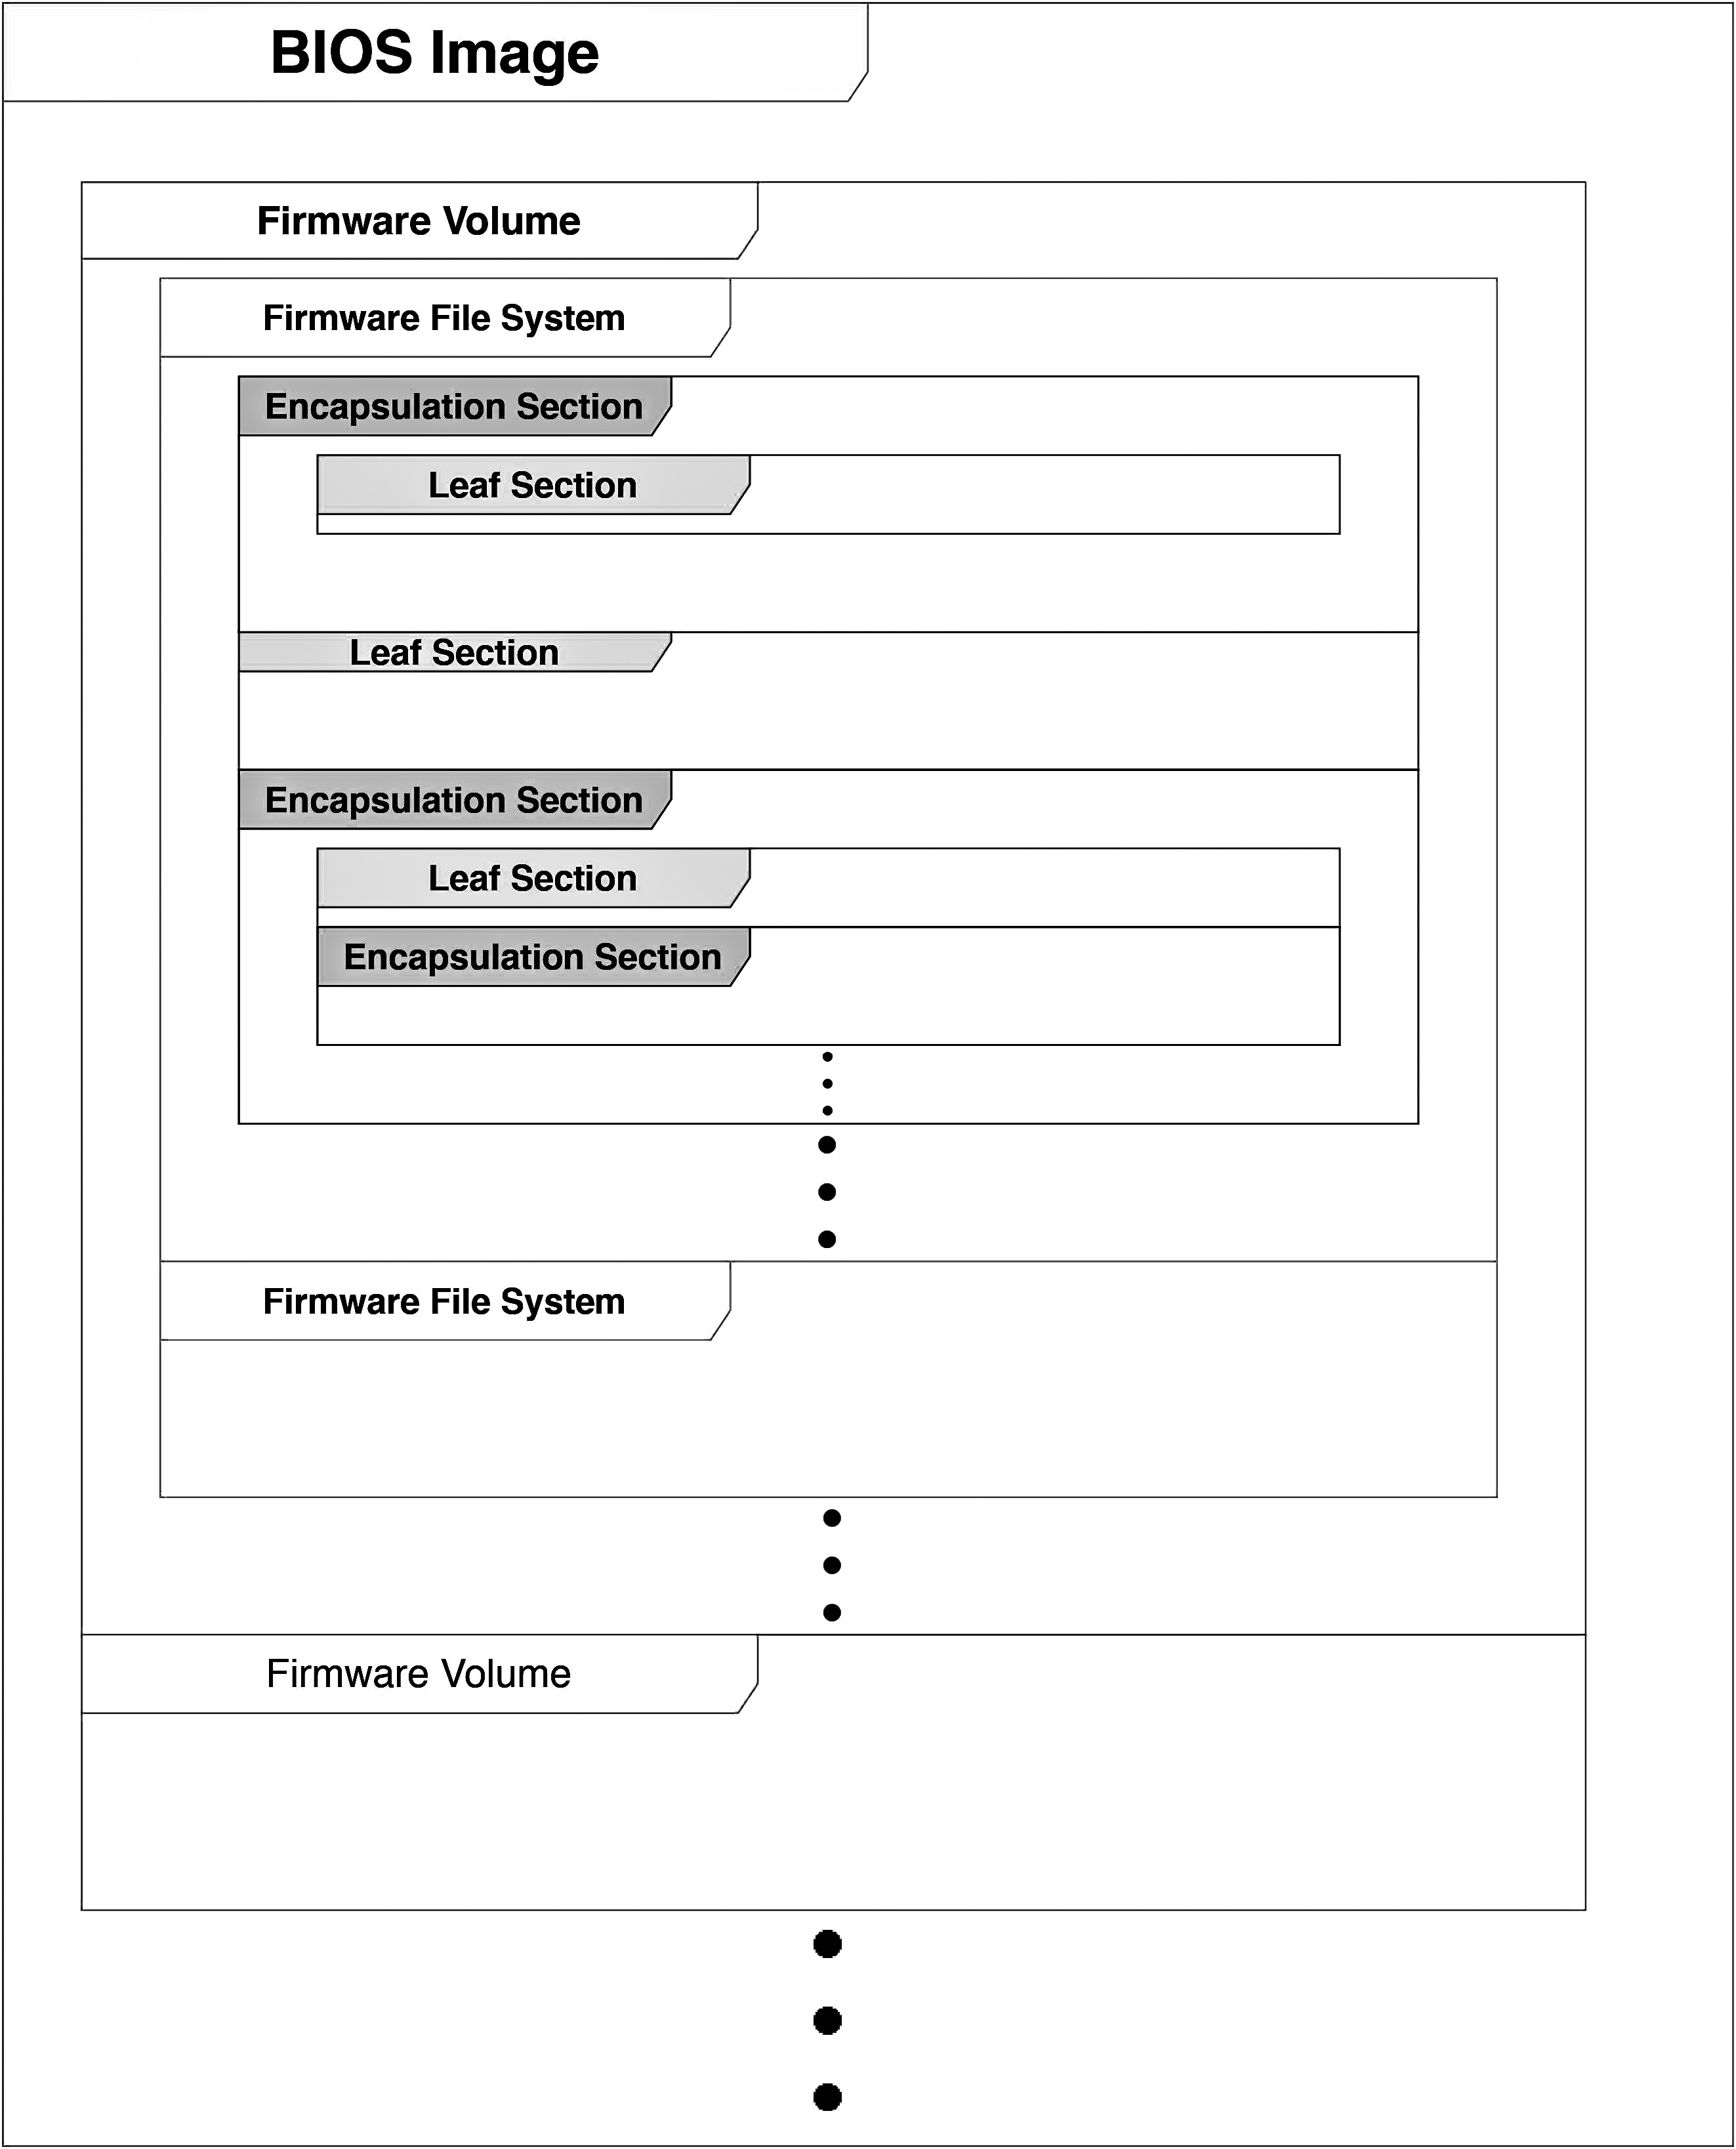
\includegraphics[width=\linewidth]{proposed-work/bios-as-filesystem}
	\caption{Overview of BIOS image as a File System}\label{fig:bios-as-filesystem}
\end{figure}

\subsubsection{Additional Tech Stack Used}
Below are the listed technologies consumed in development of this module in addition to the already specified requirements in Section \ref{subsection-requirements}
\begin{itemize}
	\item Decompression binaries
	\item XML
	\item JSON
\end{itemize}

\subsubsection{Flow of the module}
Figure \ref{fig:uefi-parser} describes the flow of the Parsing module. The Initial part is performed by user who is responsible to select valid memory interface to work. Note that some memory interface are supported by the module which requires additional hardware and software setup which are considered to be the part of dependency of interface itself which is not in the scope of the module.

When User select valid Interface the module will determine whether user is on Target \gls{sut} or on the local BIOS image.
If user is working on SUT with valid memory interface and privileges then BIOS image will be parsed from the memory.

\begin{figure}[!htbp]
	\centering
	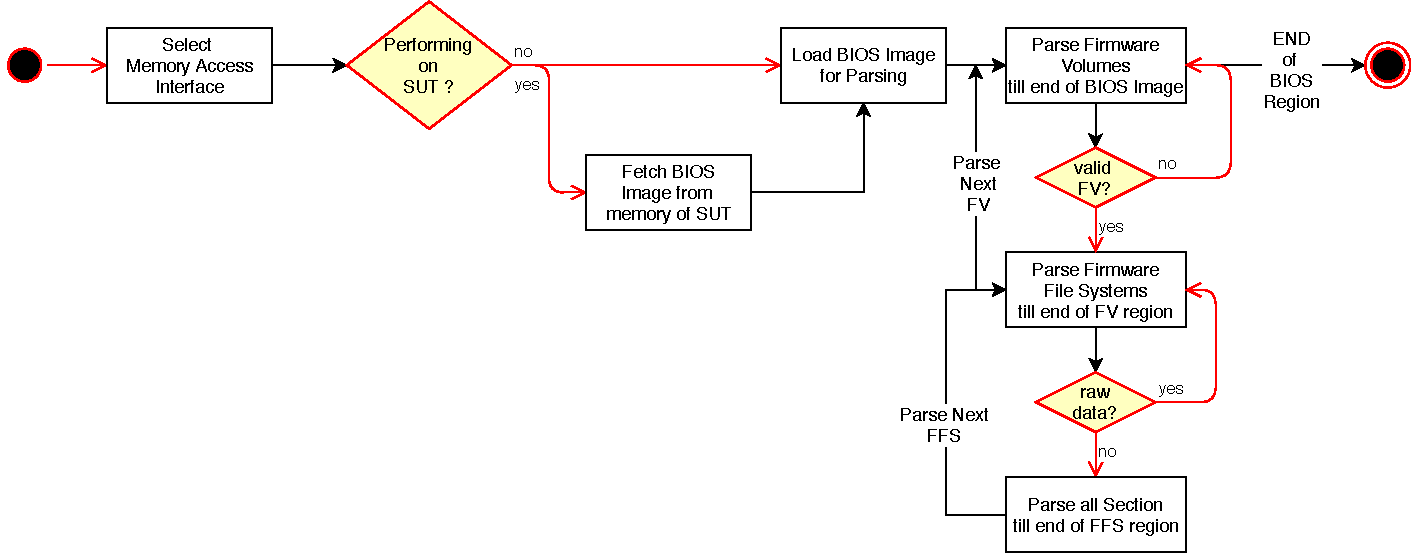
\includegraphics[width=\linewidth]{proposed-work/uefi-parser}
	\caption{Flow of Parser}\label{fig:uefi-parser}
\end{figure}

As on both the cases BIOS Image is available to act on, the module will start the parsing of the BIOS image as interpretation described in Figure \ref{fig:bios-as-filesystem}. It parses All the valid firmware volumes only till the end of BIOS image (skips the free space or firmware volumes with invalid signature and GUID). Decompression of file system under the firmware volume if any is handled by the module too, for the decompression of file system it uses the binary for decompression technique available to public i.e. lzma, tianocore, brotli etc.


\subsubsection{Outcome of Module}
\begin{itemize}
	\item Human Readable interpretation of BIOS image is provided.
	\item Possible to debug the BIOS via setup knobs comparison.
	\item Lookup of order of the module in BIOS image as readable file system is also possible.
	\item Verification of integration of module via GUID can be done.
	\item Extracting and storing file system or module of BIOS image by GUID
	\item Summarizing changes of two BIOS image
\end{itemize}



% ========================================================================
% MODULE 3
% ========================================================================
\subsection{Module: Runtime UEFI variable Creation}\label{module-runtime-uefi-variable-creation}
Each variable in BIOS has a scope for each variable where Runtime support is one of the attribute, to simply state the run time variable one can interpret it as the variable which will be available during and after the completion boot flow (while OS is running). Such a variable require special access mechanism, which is carried out by the System Management mode \gls{smm} described in Section \ref{section-smm}.

Earlier Challenges are described as below:
\begin{itemize}
	\item Providing and maintaining native driver support from BIOS for creation of UEFI variable
	\item Setting of Build environment for non-BIOS development team
\end{itemize}

Note: As all the variable created at runtime the scope of such variable are limited to the flashing of the BIOS. i.e. when BIOS is flashed/re-flashed or updated, those variable won't be available on the SUT.

\subsubsection{Additional Tech Stack Used}
Below are the listed technologies consumed in development of this module in addition to the already specified requirements in Section \ref{subsection-requirements}
\begin{itemize}
	\item Flask
	\item Ajax
	\item jQuery
	\item Javascript
	\item HTML/CSS
	\item XML
	\item JSON
\end{itemize}

\subsubsection{Flow of the module}
\begin{figure}[!htbp]
	\centering
	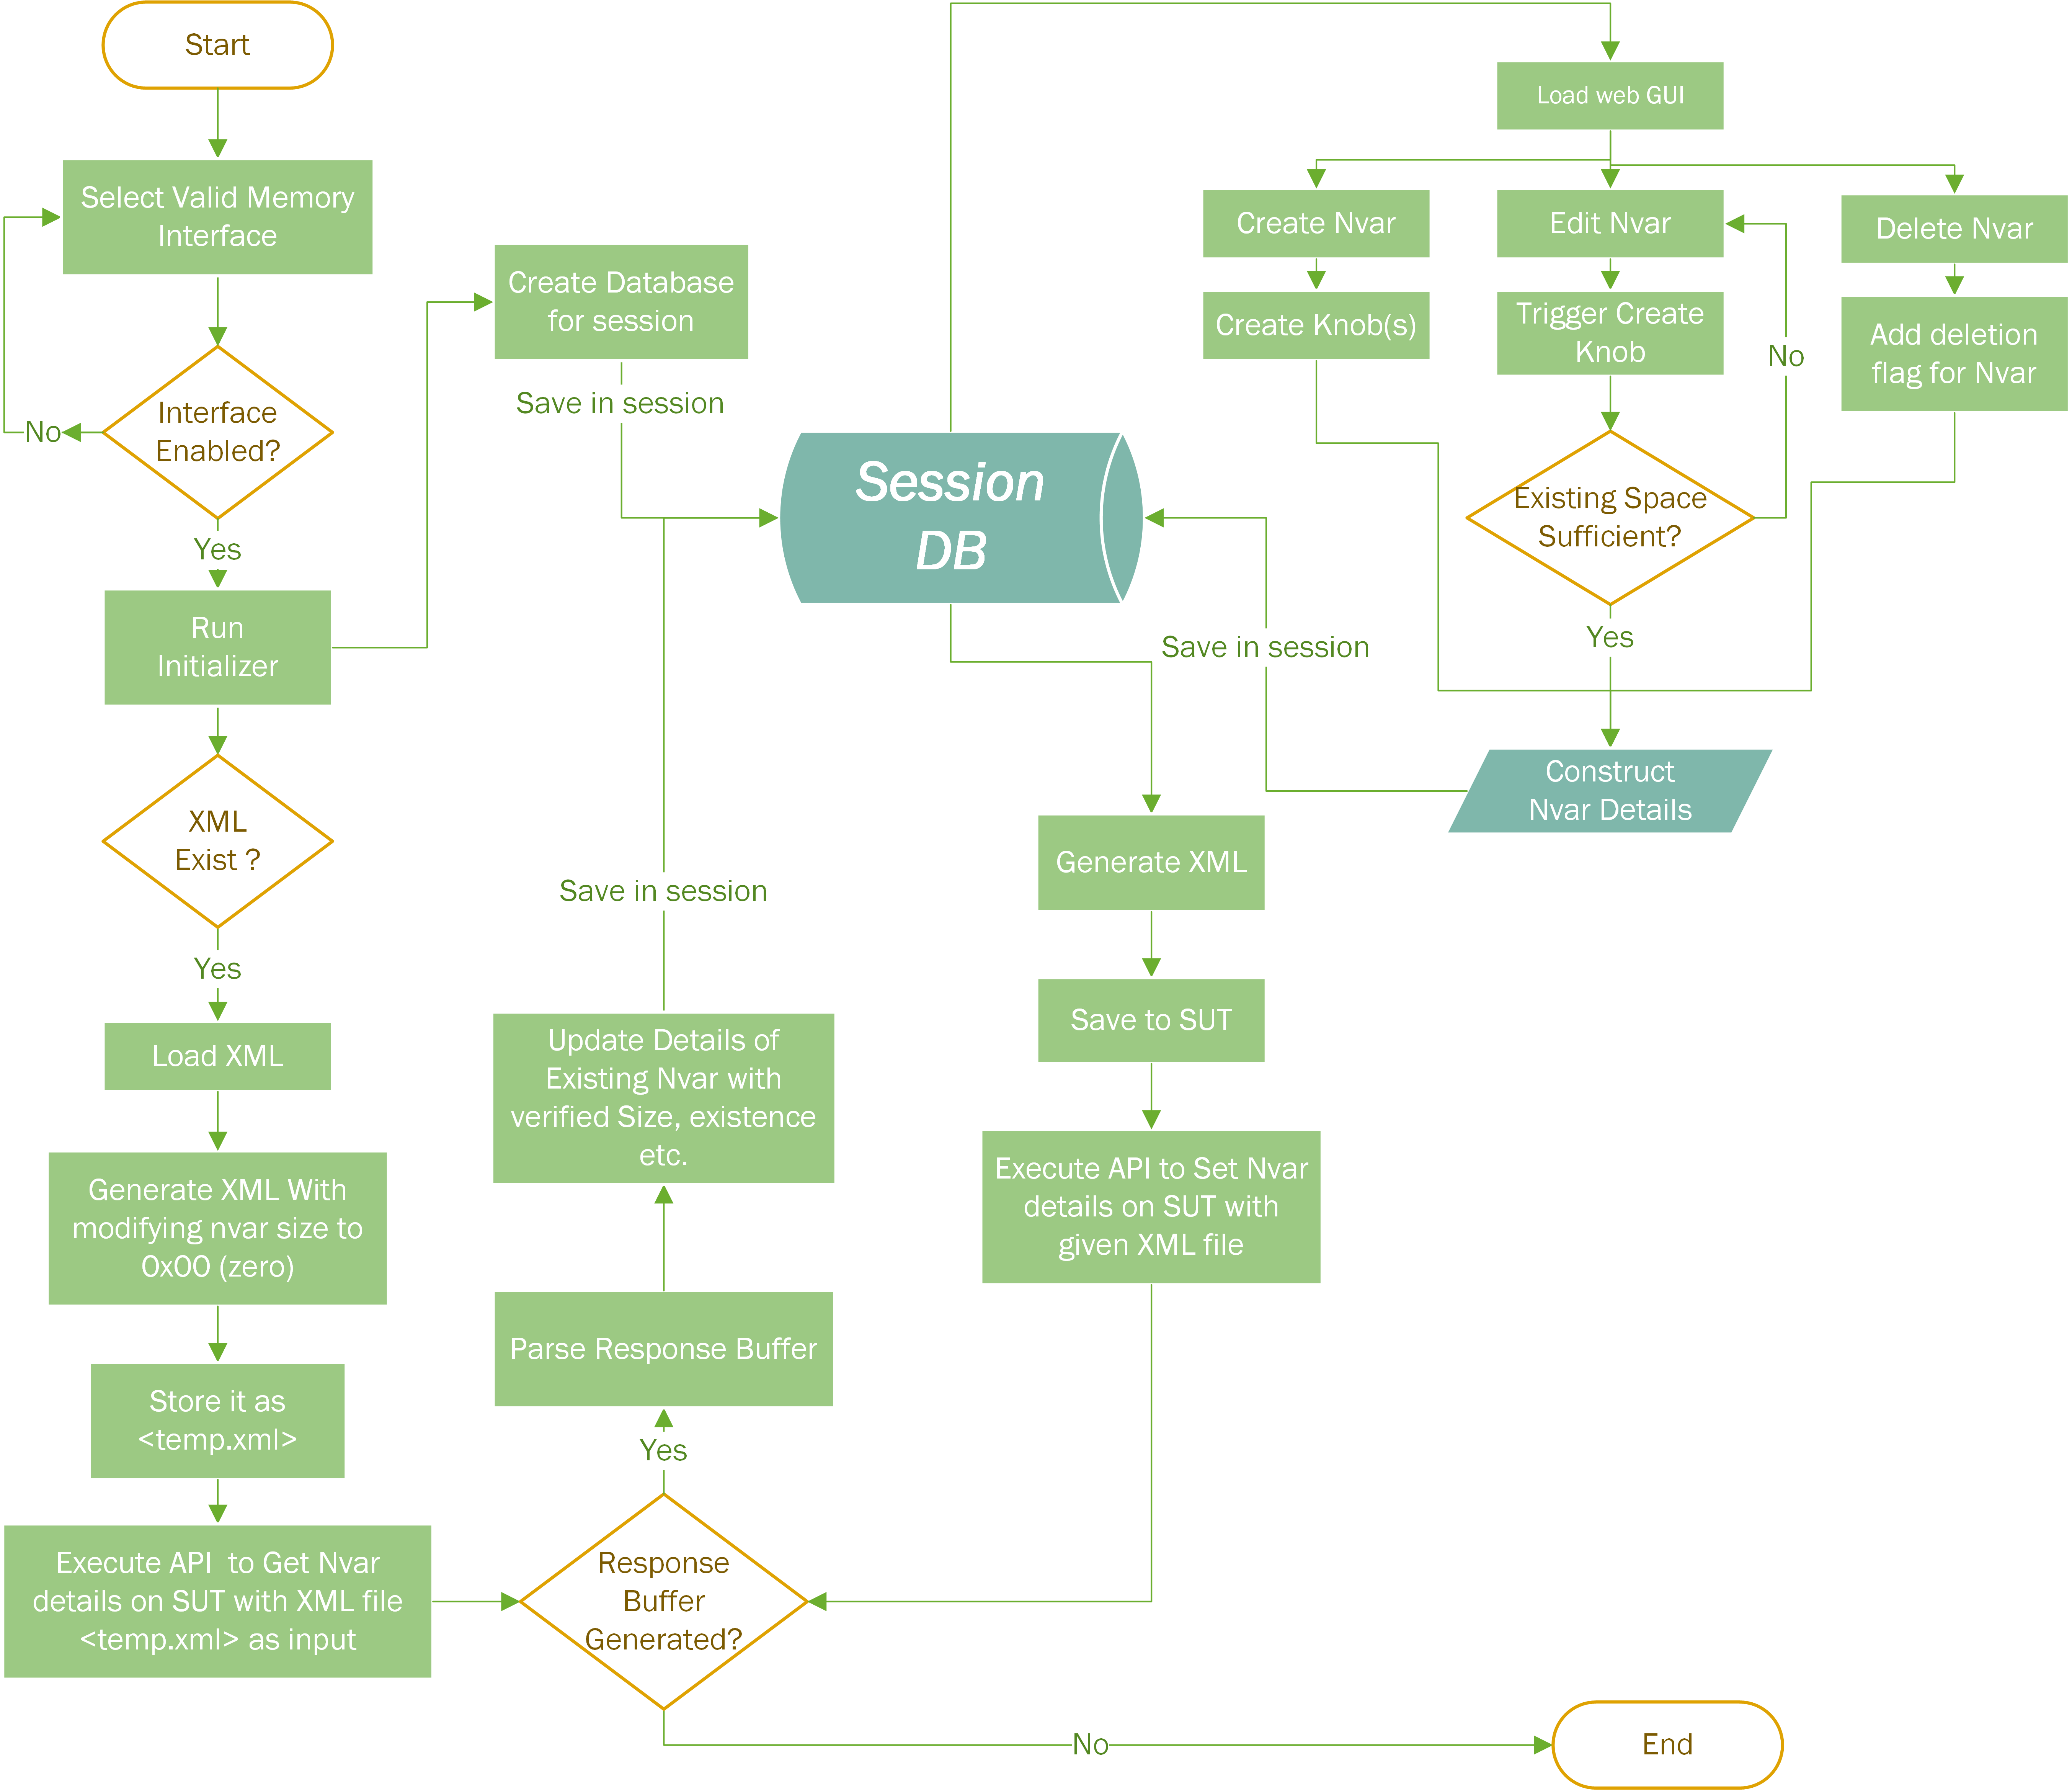
\includegraphics[width=1\linewidth]{proposed-work/nvar_web_GUI_flow}
	\caption{Flow of Nvar Web GUI}\label{fig:nvar_web_GUI_flow}
\end{figure}
The Flow of the module is described in section \ref{subsubsection-screenshots} along with screenshots which is easier to interpret the flow chart in Figure \ref{fig:nvar_web_GUI_flow}.

\subsubsection{Screenshots of Module}\label{subsubsection-screenshots}
Whenever the User launches the module the home page screen to select valid communication interface will appear as displayed in Figure \ref{fig:uefi-variable-home}. This is the crucial stage as if valid interface for communication is not selected one may not be able to use the functionality of the service.

\begin{figure}[!htbp]
	\centering
	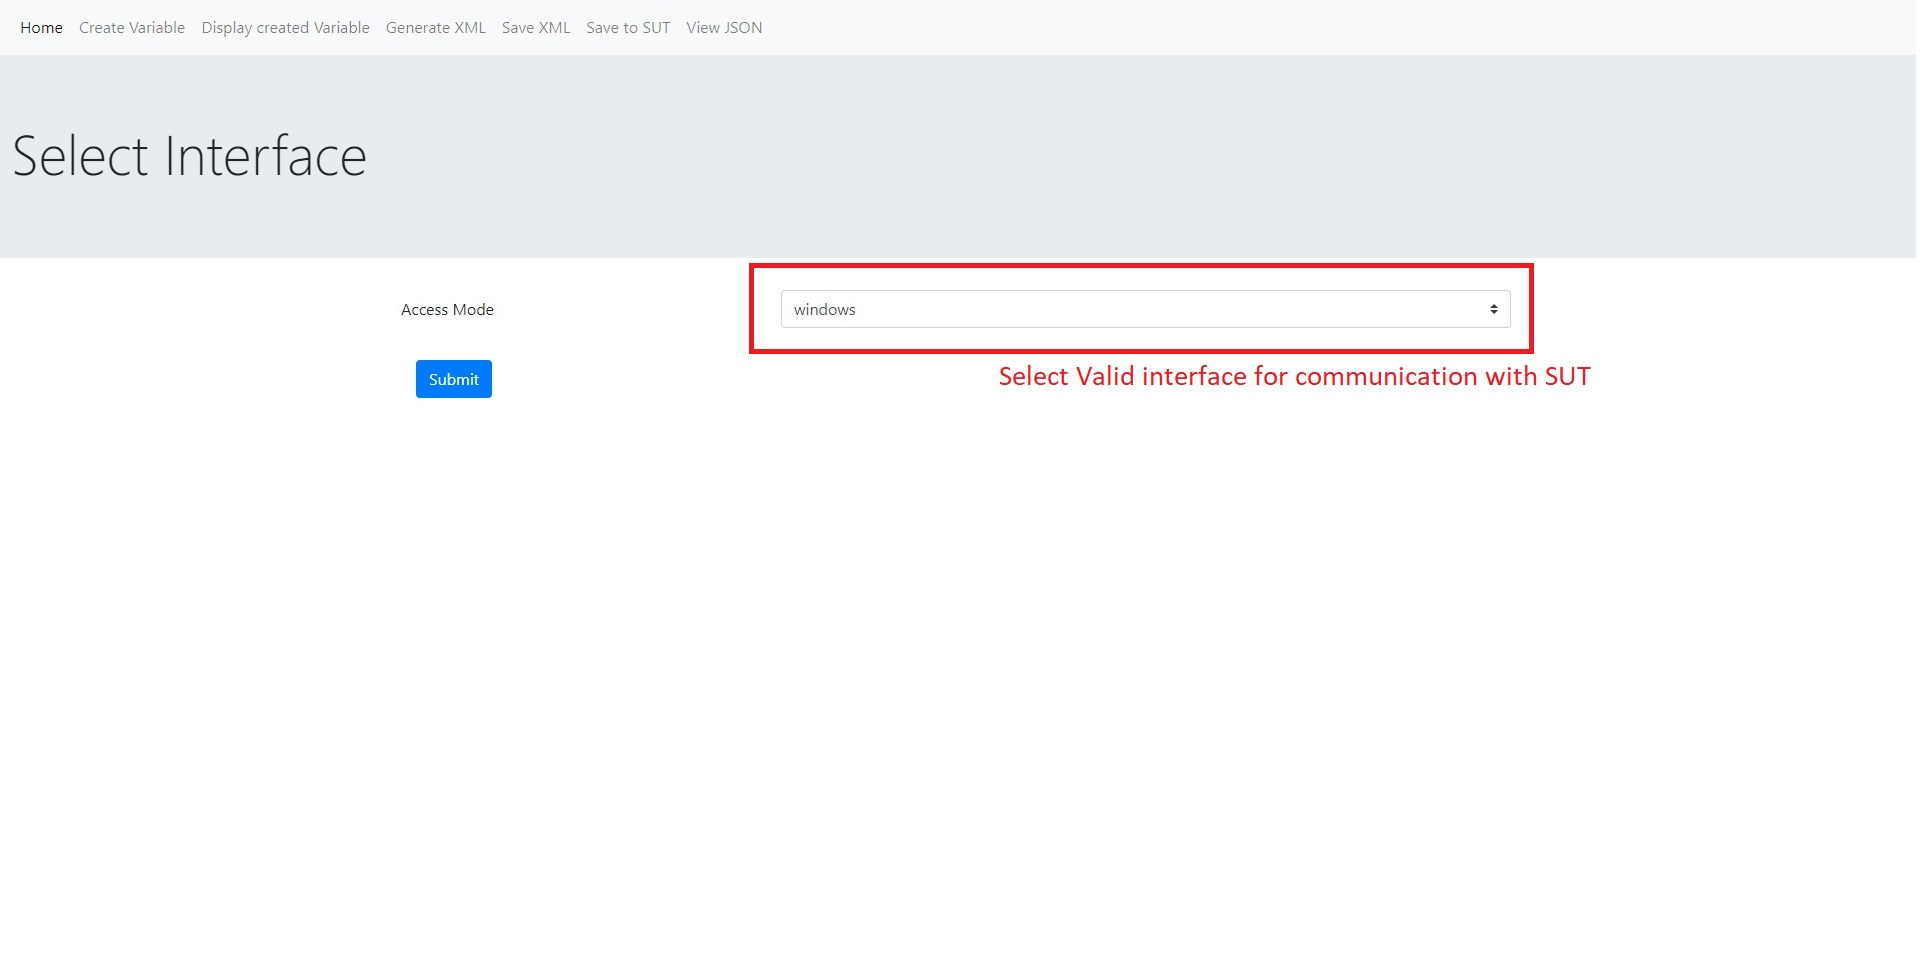
\includegraphics[width=\linewidth]{proposed-work/uefi-variables/home}
	\caption{Home Page to Create UEFI Variable}\label{fig:uefi-variable-home}
\end{figure}

After selection of valid Interface one may operate the desired options listed in navigation bar which are:

\begin{table}
	\centering
	\renewcommand{\arraystretch}{2}
	\caption{Navigation Bar Action}\label{table:navbar-action}
	\begin{tabular}{l | p {8cm}}
		Button & Interpretation
		\\ \hline \hline
		Create Variable & Opens a form to create new Variable as in Figure \ref{fig:uefi-variable-create-nvar}
		\\ \hline Display Created Variable & lists out created variable as in Figure \ref{fig:uefi-variable-created-option}
		\\ \hline Generate XML & Generate XML from the stored session database as in Figure \ref{fig:uefi-variable-generate-xml}
		\\ \hline Save XML & Saves the generated XML on the storage device
		\\ \hline Save to SUT & Applies the Pending changes action (Create/Delete/Modify) to the \gls{sut}
		\\ \hline View JSON & View the stored session database in the json format as in Figure \ref{fig:uefi-variable-represent-json}
		\\ \hline
	\end{tabular}
\end{table}


Figure \ref{fig:uefi-variable-created-option} lists the variable created under the current session which is to be applied 
\begin{figure}[!htbp]
	\centering
	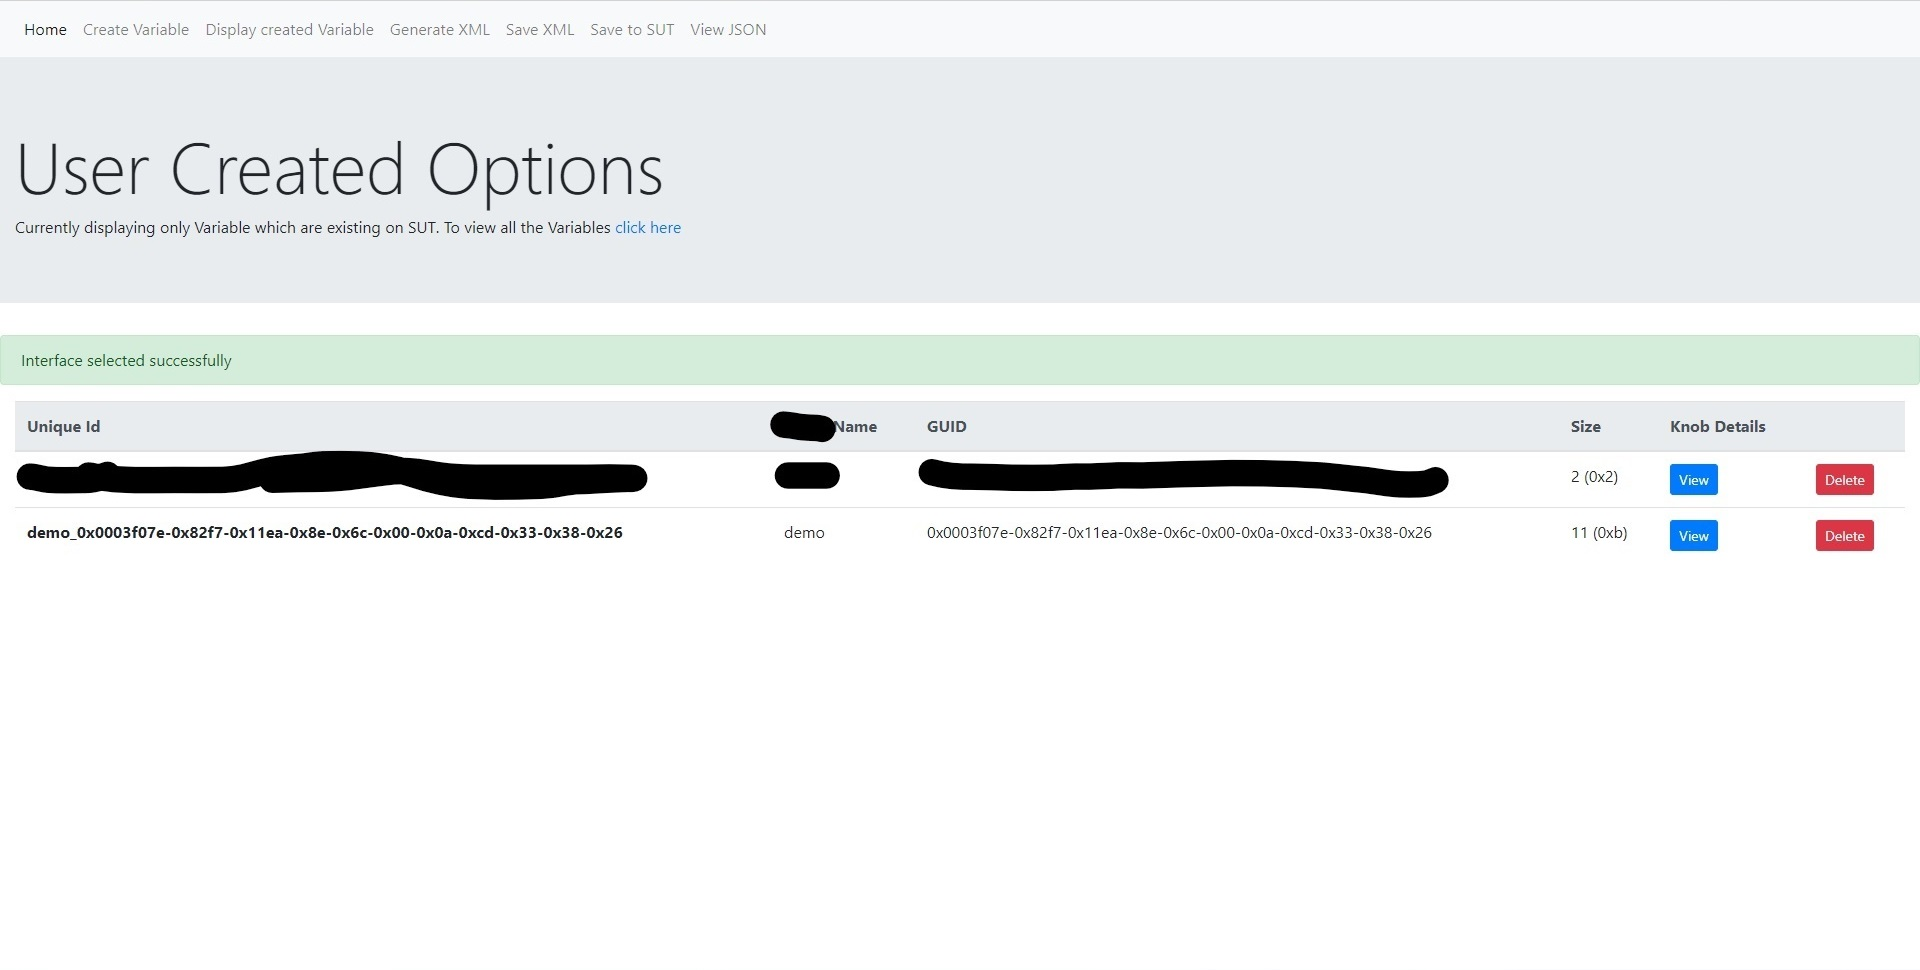
\includegraphics[width=\linewidth]{proposed-work/uefi-variables/created-option}
	\caption{Variables created or exists on \gls{sut}}\label{fig:uefi-variable-created-option}
\end{figure}

Figure \ref{fig:uefi-variable-create-nvar} displays form which allows user to create Variable, where user needs to specify the name of the variable with certain restriction of input field. To identify and lookup the Variable the GUID is required which is automatically generated by the module with required format, however if user wishes then they can modify the GUID.
\begin{figure}[!htbp]
	\centering
	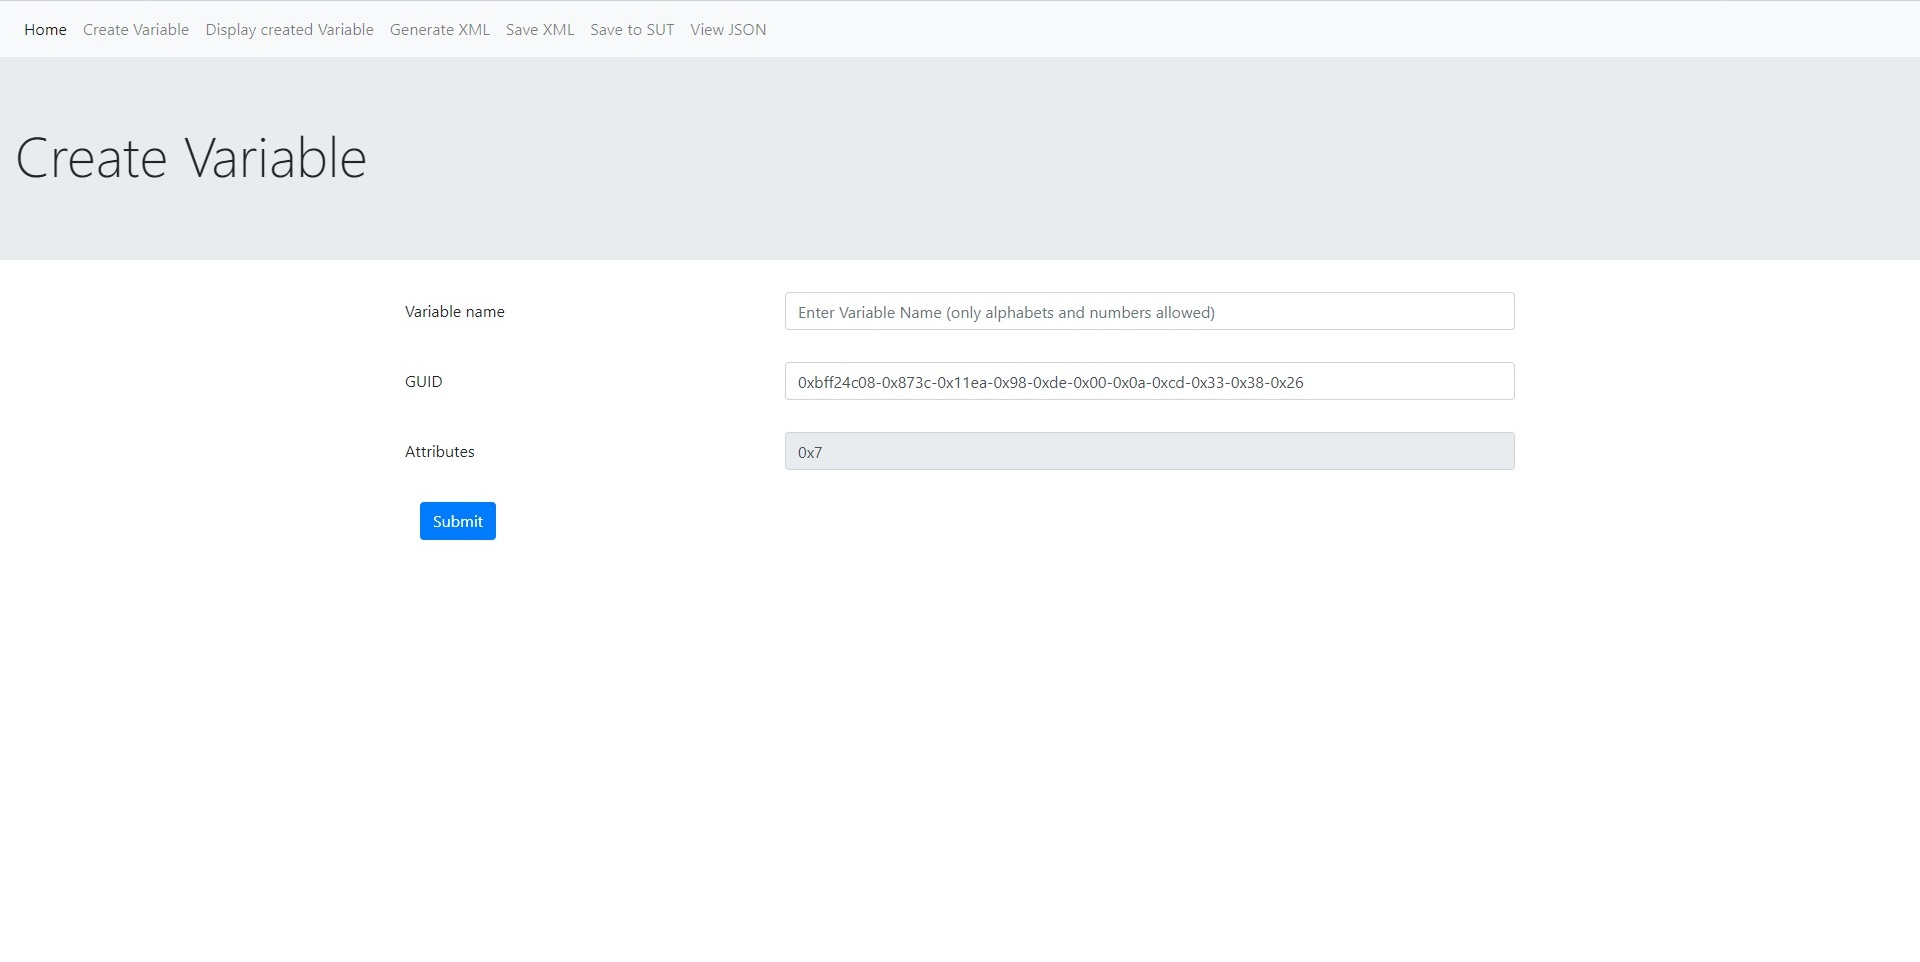
\includegraphics[width=\linewidth]{proposed-work/uefi-variables/create-nvar}
	\caption{Create new UEFI Variable on \gls{sut}}\label{fig:uefi-variable-create-nvar}
\end{figure}


Figure \ref{fig:uefi-variable-var-options} opens the list of the options if created and allows to edit their current values too. However one can also add the new option to the Variable. It allows user to create various types of options under the variable which are oneof type as in Figure \ref{fig:uefi-variable-add-option}, string type as in Figure \ref{fig:uefi-variable-string}, numeric type as in Figure \ref{fig:uefi-variable-numeric} and the checkbox type which allows user to toggle the option value in as Boolean interpretation. Common fields for creating options including its name, type, description and size.
\begin{figure}[!htbp]
	\centering
	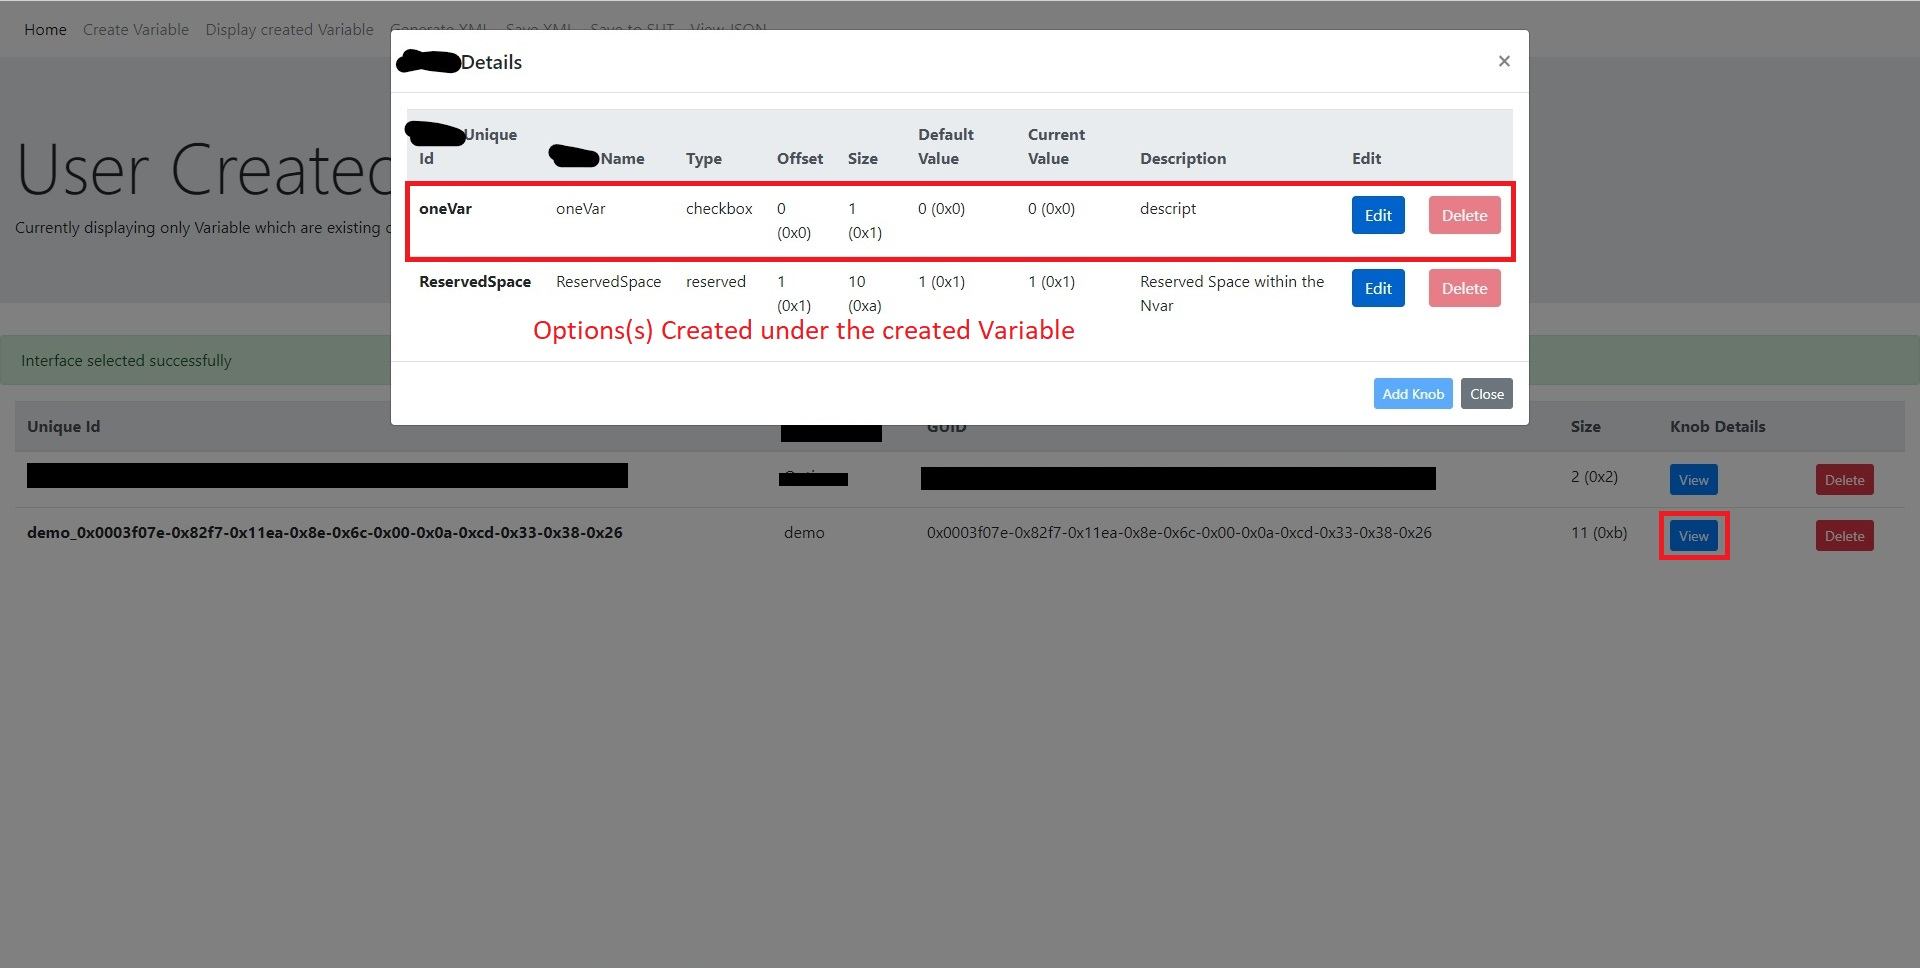
\includegraphics[width=\linewidth]{proposed-work/uefi-variables/var-options}
	\caption{Options listed under Variable}\label{fig:uefi-variable-var-options}
\end{figure}

If user wants to change the value set for the variable created while creation of option as described in Figure \ref{fig:uefi-variable-edit-option} forms one can actually modify the value.
\begin{figure}[!htbp]
	\centering
	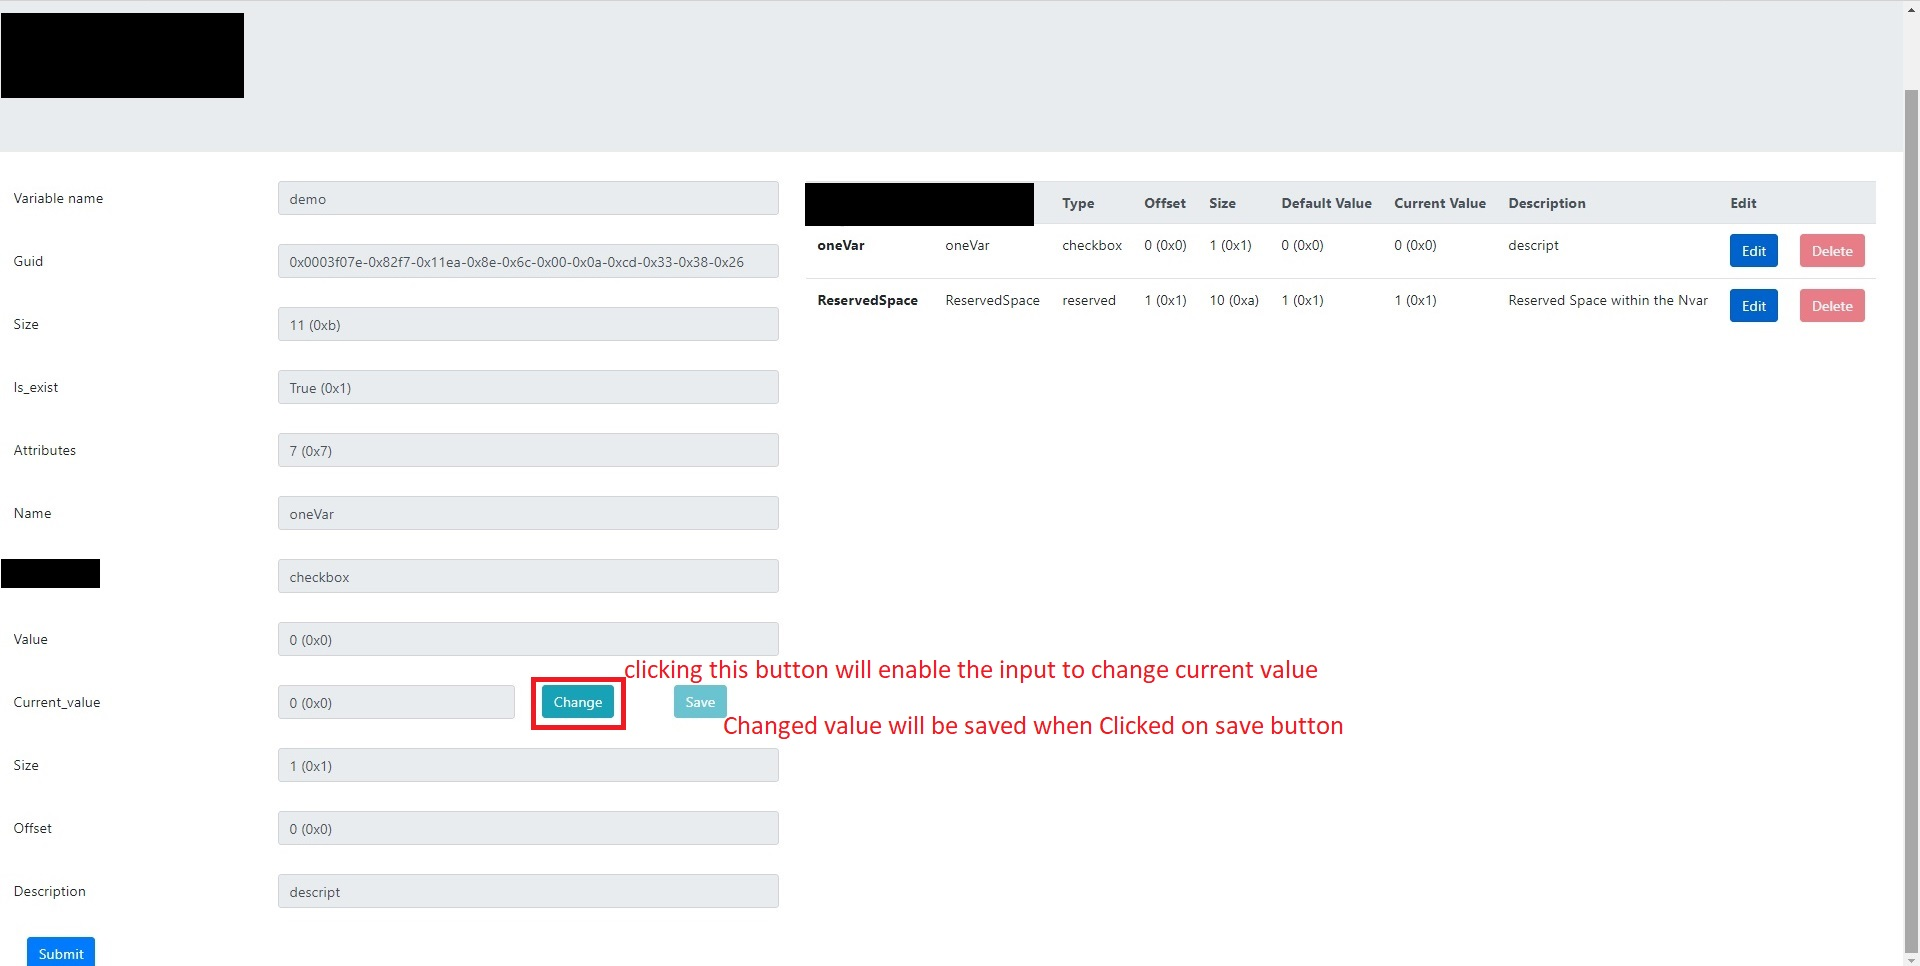
\includegraphics[width=\linewidth]{proposed-work/uefi-variables/edit-option}
	\caption{Edit the Existing Option Created under Variable \gls{sut}}\label{fig:uefi-variable-edit-option}
\end{figure}

The highlighted prompt in Figure \ref{fig:uefi-variable-add-option} allows user to create the choices for the option where one of the multiple values to be selected as a result, By clicking \verb|Add Option| button user can create choices and under drop down menu besides Value, user can select default value to be selected for the option. 
\begin{figure}[!htbp]
	\centering
	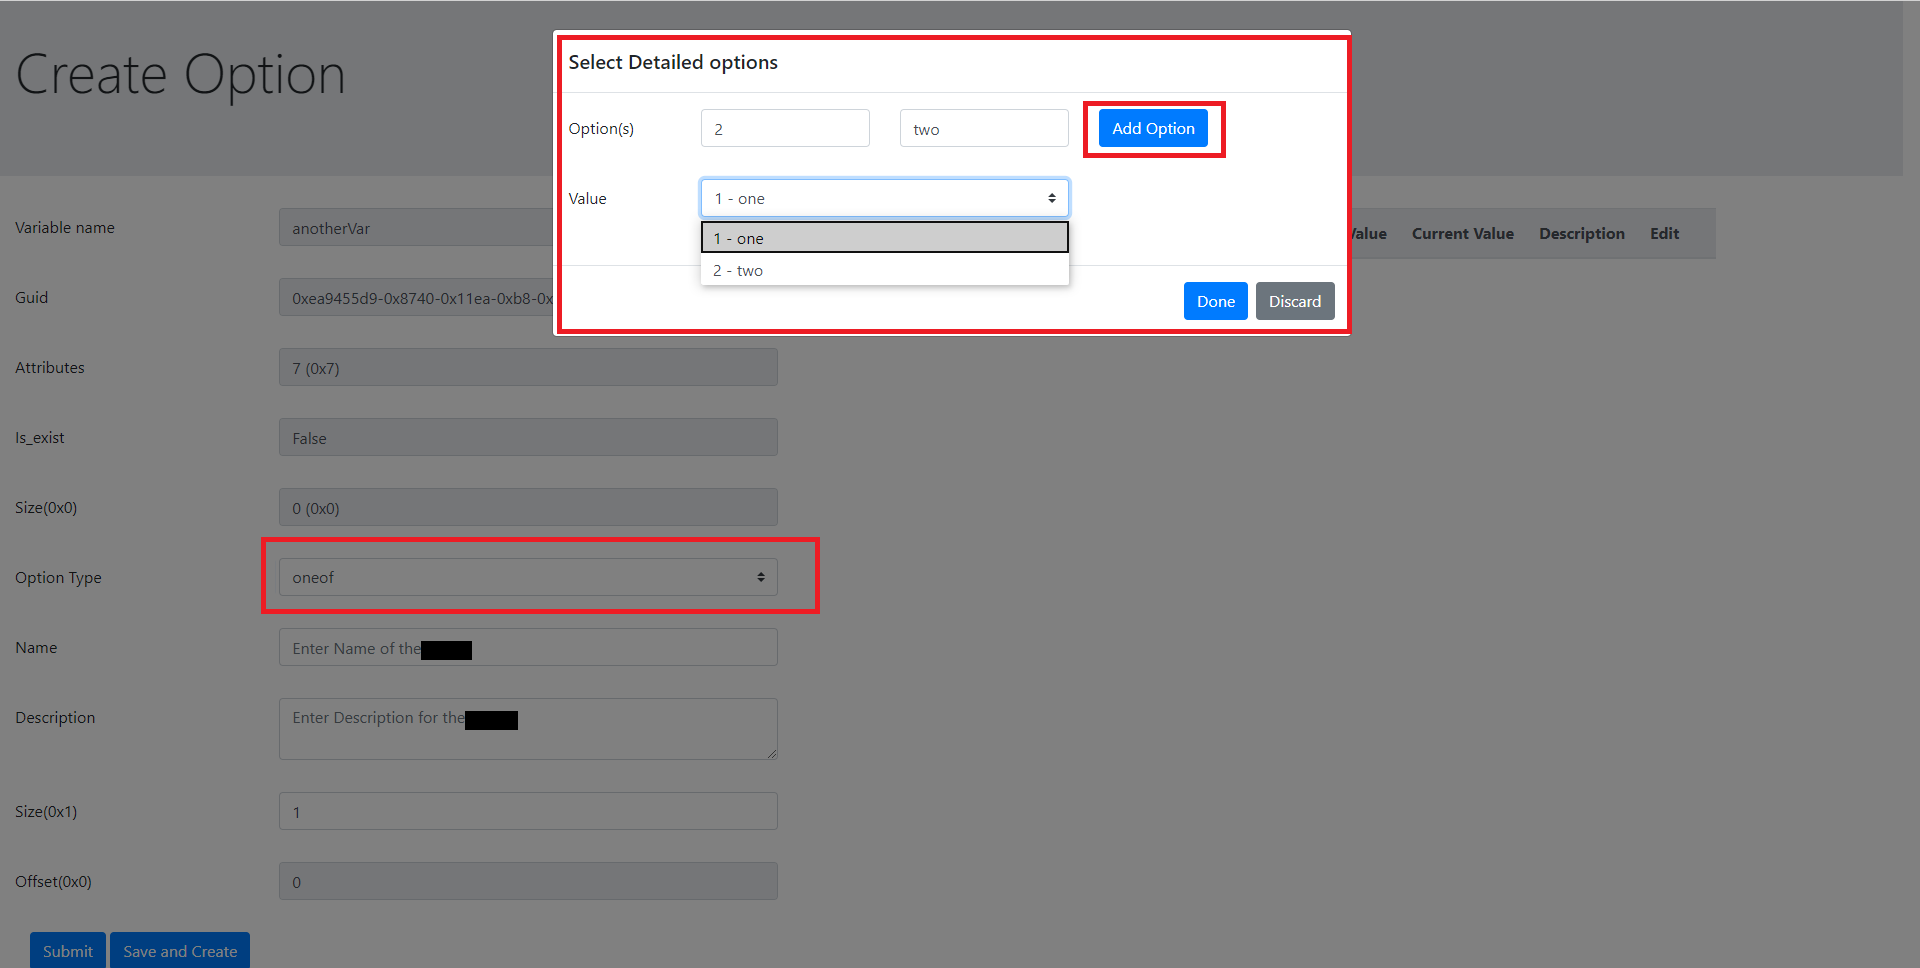
\includegraphics[width=\linewidth]{proposed-work/uefi-variables/add-option}
	\caption{Create New Option(s) under Variable - Oneof Type}\label{fig:uefi-variable-add-option}
\end{figure}

Option type string as in Figure \ref{fig:uefi-variable-string} allows user to create a option which accepts minimum and maximum characters to be supported in the string as well as the default string value to be selected. 
\begin{figure}[!htbp]
	\centering
	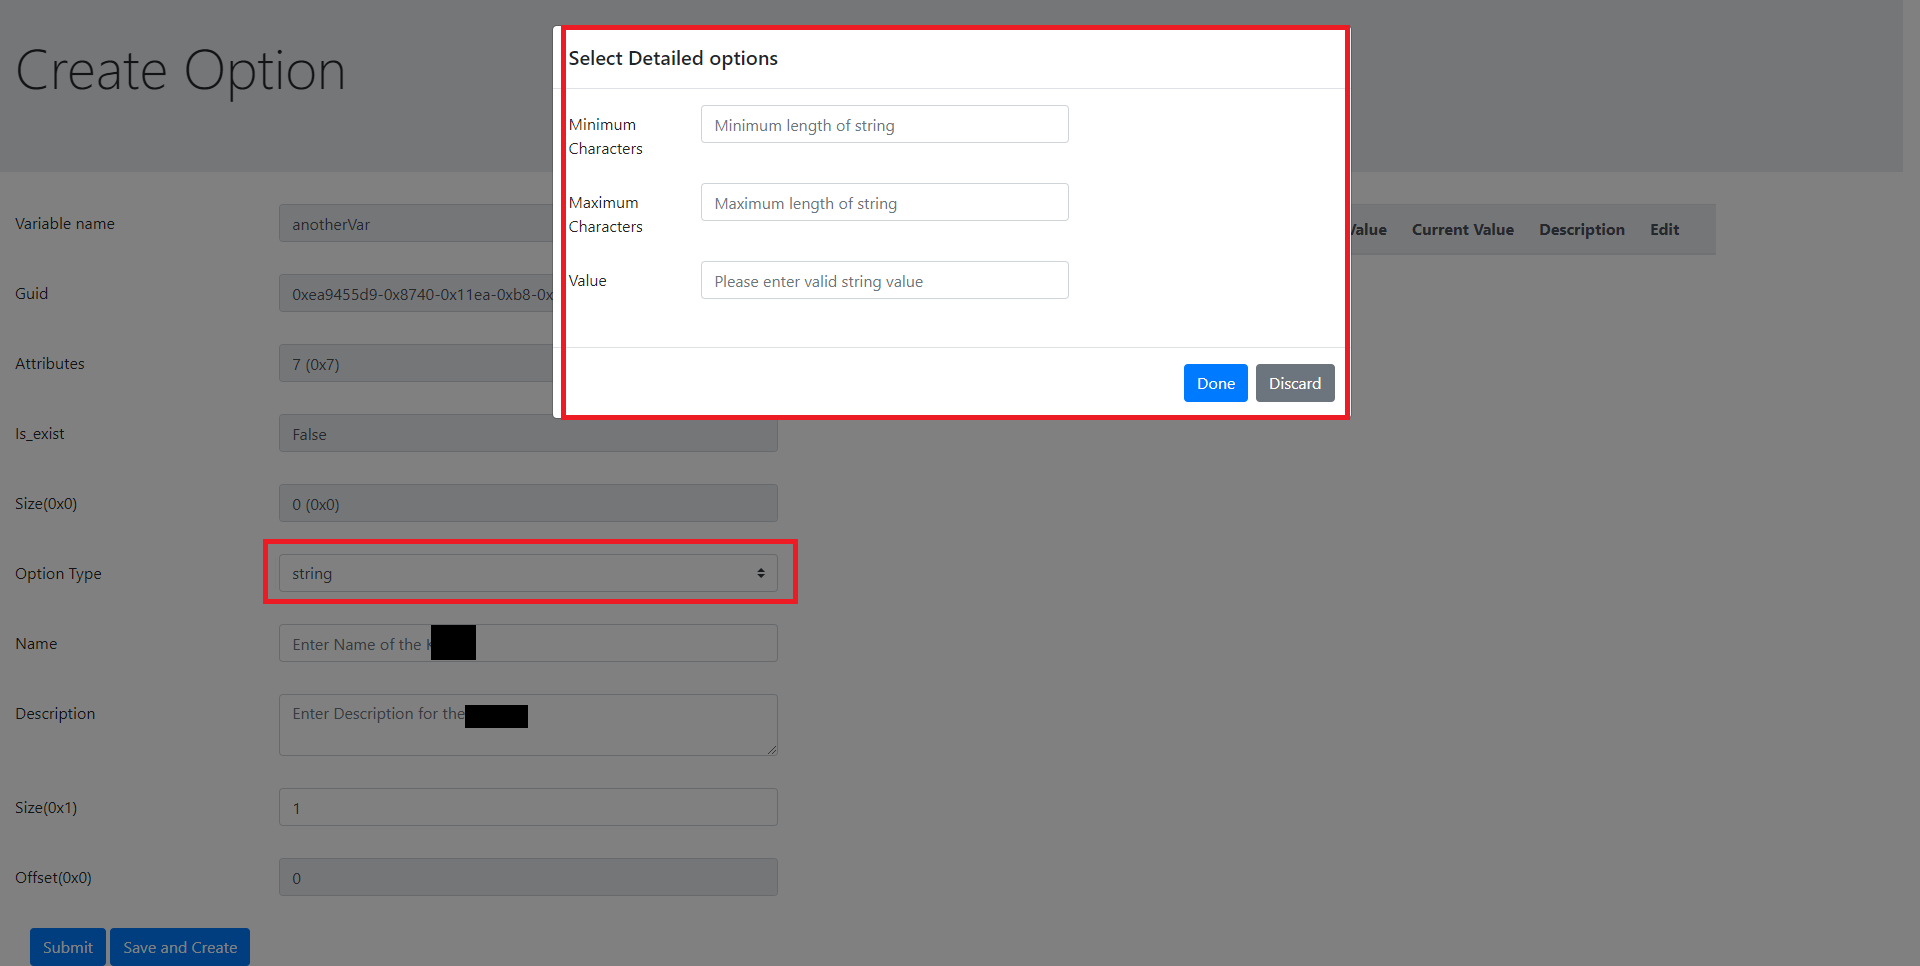
\includegraphics[width=\linewidth]{proposed-work/uefi-variables/string}
	\caption{Create New Option(s) under Variable - String Type}\label{fig:uefi-variable-string}
\end{figure}

To set the numeric input for the option, minimum and maximum value along with the default value to be set as in Figure \ref{fig:uefi-variable-numeric}
\begin{figure}[!htbp]
	\centering
	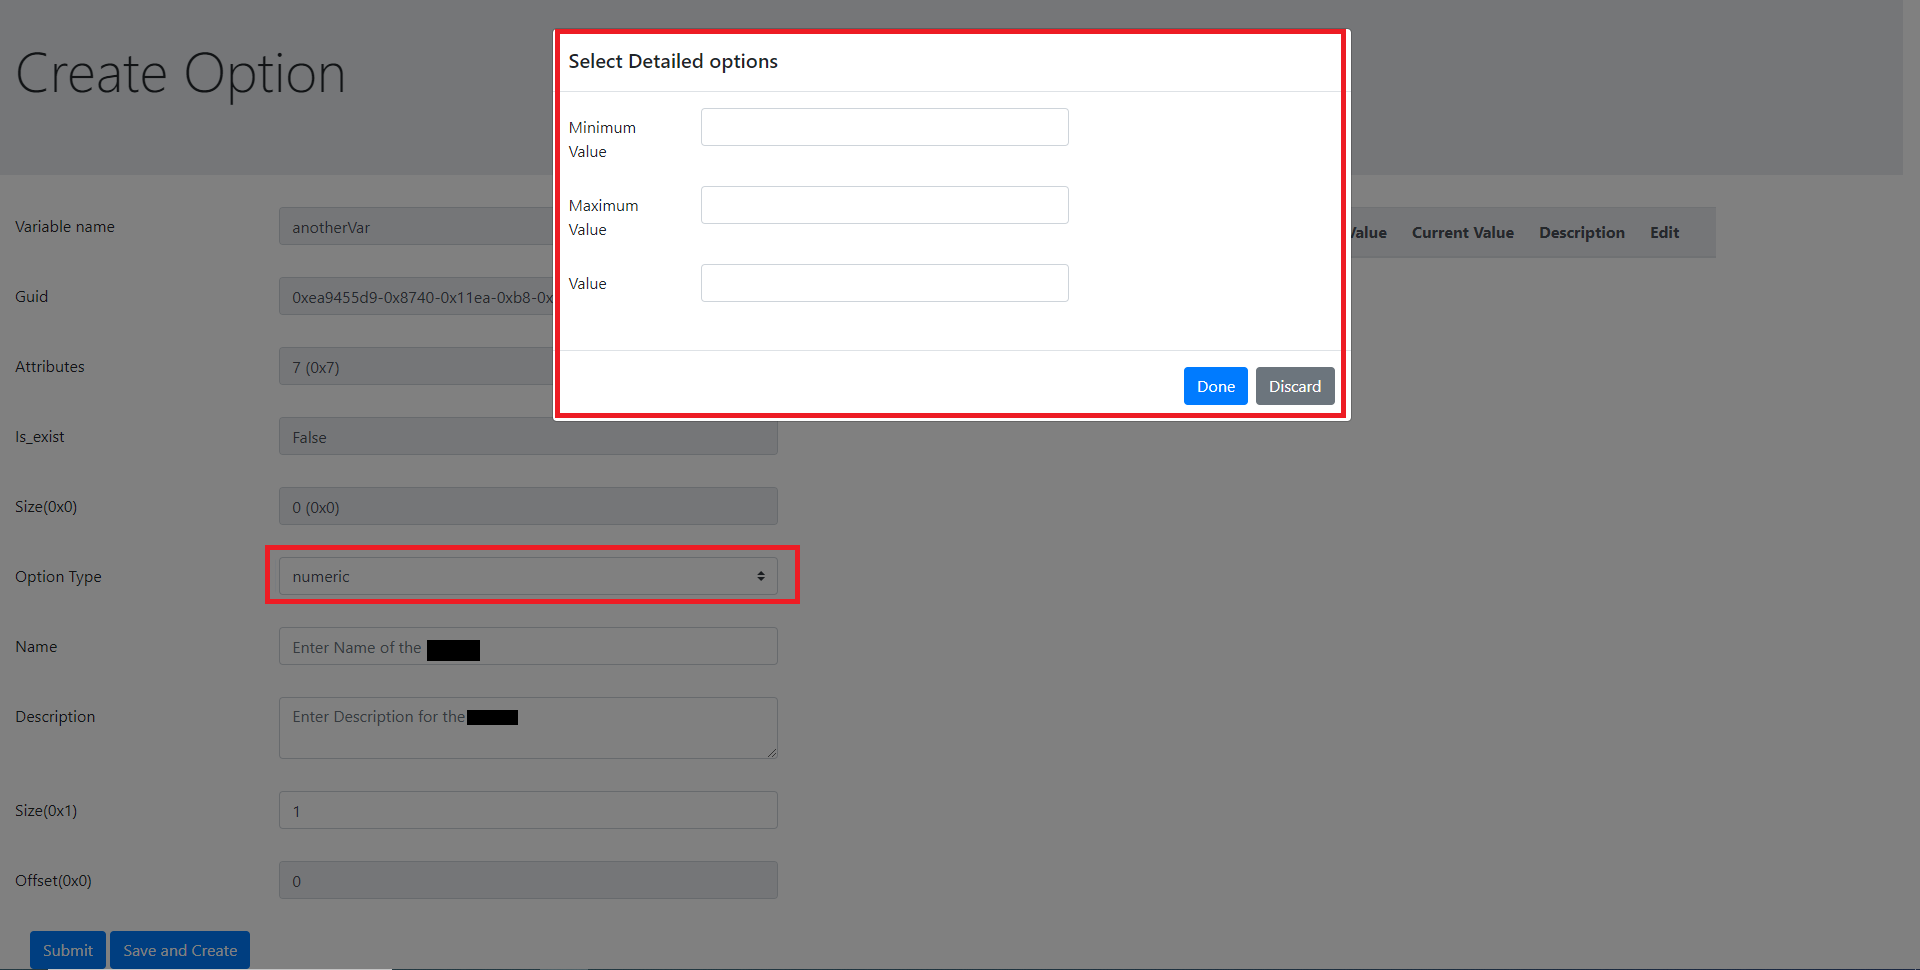
\includegraphics[width=\linewidth]{proposed-work/uefi-variables/numeric}
	\caption{Create New Option(s) under Variable - Numeric Type}\label{fig:uefi-variable-numeric}
\end{figure}

For the future use one can create a reserved space under the UEFI variable as in Figure \ref{fig:uefi-variable-reserved-space}
\begin{figure}[!htbp]
	\centering
	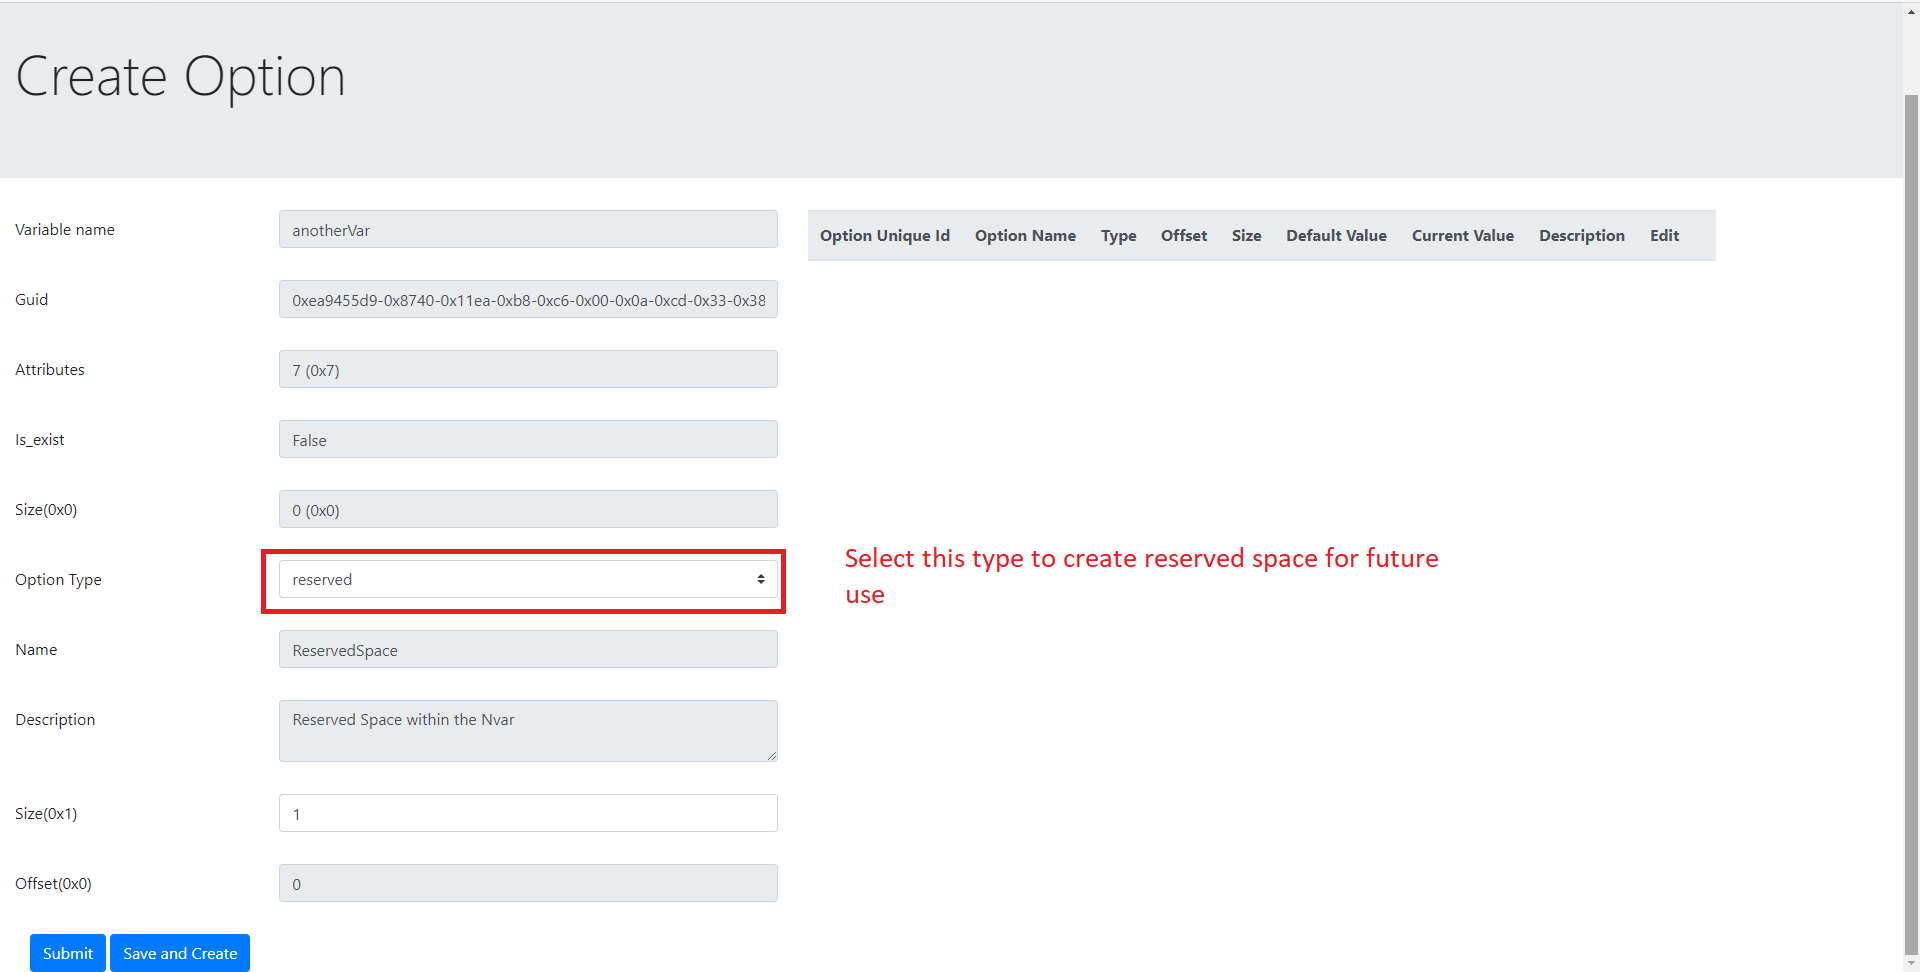
\includegraphics[width=\linewidth]{proposed-work/uefi-variables/reserved-space}
	\caption{Create Reserved Space for future use under Variable}\label{fig:uefi-variable-reserved-space}
\end{figure}


Figure \ref{fig:uefi-variable-generate-xml} shows the XML which is generated from the existing and newly created variables and options under it.
\begin{figure}[!htbp]
	\centering
	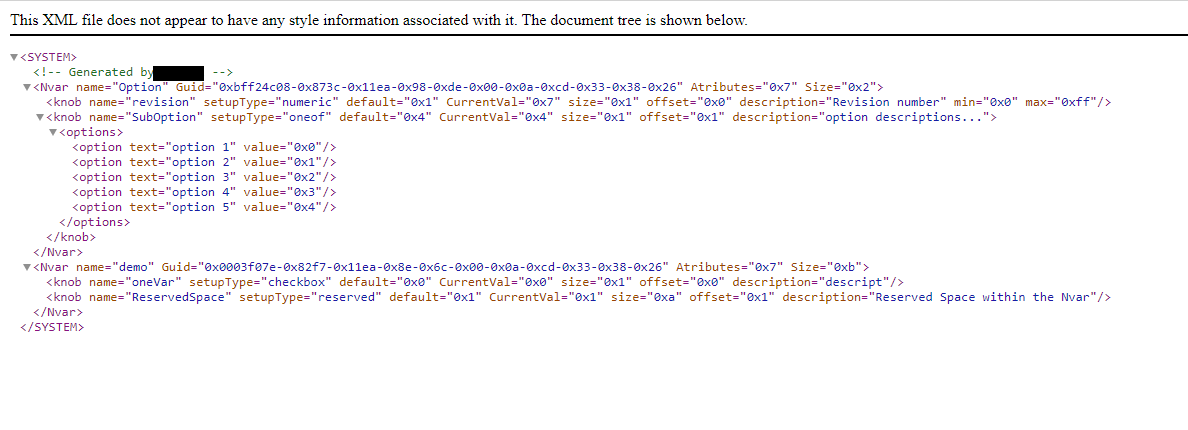
\includegraphics[width=\linewidth]{proposed-work/uefi-variables/generate-xml}
	\caption{Generate XML \gls{sut}}\label{fig:uefi-variable-generate-xml}
\end{figure}

Figure \ref{fig:uefi-variable-represent-json} represents session data of existing and newly created data (if any) as json
\begin{figure}[!htbp]
	\centering
	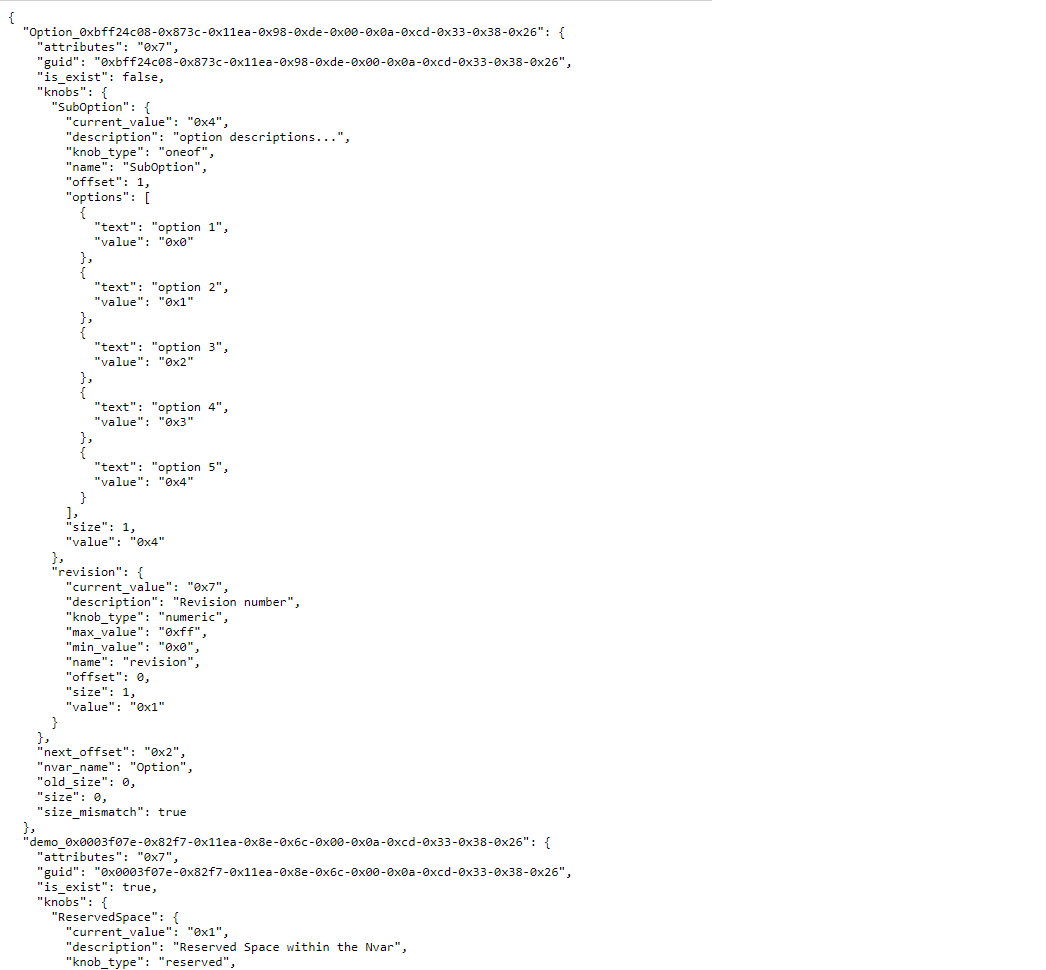
\includegraphics[width=\linewidth]{proposed-work/uefi-variables/represent-json}
	\caption{Generate XML \gls{sut}}\label{fig:uefi-variable-represent-json}
\end{figure}


\subsubsection{Outcome of the module}
\begin{itemize}
	\item Enables creation of UEFI variable from OS layer.
	\item Lifts headache of maintaining variable creation from BIOS development for individuals.
\end{itemize}



\section{Future Scope of Work}\label{section-future-scope}
Section \ref{subsection-processing-bios} so far covered only a framework with single module only to back the proposed work with the \gls{poc}. 
However the next phase of the existing work will include:
\begin{itemize}
	\item Study of existing hotspots for automation
	\item Analyzing and gathering requirements of automation to hotspot
	\item Implementing and managing platform to keep up-to-date the user base of the framework
\end{itemize}

The study also shows the redundant implementation definition of codebase and structure under various different platform architecture and components. Thus the another possible scope of can be the implementation of a reinforcement algorithm to perform optimizing the redundant codebase across all the platforms by maintaining the integrity and security as per \gls{csme} guideline.


\clearpage
\printglossary[type=main]
%\printnoidxglossaries[type=main]
\end{document}